\chapter{Mockups und Implementierung}\label{ch:mockups-und-implementierung}
Im Folgenden werden die Mockups für die Anforderungen des dritten Releases vorgestellt.
Das jeweilige Mockup wird beschrieben und auf Einzelheiten bezüglich der Anforderung eingegangen.
Darüber hinaus wird das Mockup mit seiner tatsächlichen Implementierung verglichen. Dabei wird es nur auf Unterschiede eingegangen und diese werden gegebenenfalls erläutert.

\section{Dialogsystem für NPC-Trainer}\label{sec:dialogsystem-fur-npc-trainer}
In diesem Release wird das Spiel \textit{Monster Odyssey} um ein Dialogsystem erweitert. Damit kann der Nutzer Dialoge mit NPC-Trainern führen und gegebenenfalls Aktionen mit bestimmten NPC-Trainern tätigen.
Die Aktionen können sich je nach Situation beziehungsweise angesprochenem Trainer unterscheiden.
Beispielsweise kann der Nutzer ein Starter-Monster nach dem Gespräch mit dem Trainer Prof. Albert erhalten, seine eigenen Monster bei einer Krankenschwester in einem 'Moncenter' heilen oder Kämpfe mit bestimmten NPC-Trainern starten.
\subsection{Mockups}\label{subsec:mockups-dialogsystem}
In der Abbildung~\ref{fig: User and NPC-Trainer} befindet sich der Nutzer auf einem Spielfeld und ihm steht ein NPC-Trainer gegenüber. Wenn der Nutzer einem NPC-Trainer frontal zugewandt ist, kann nach Drücken der Interaktionstaste ein Dialog gestartet werden. Der Dialog wird anschließend von dem jeweiligen NPC-Trainer geführt und in der Abbildung~\ref{fig: Dialog User and NPC-Trainer} antwortet der NPC-Trainer mit einem Beispielsatz in einem Dialogfenster: „Hey there! Did you see Pikawatch in Route 100?“. In diesem Dialogfenster sieht der Nutzer den Namen des angesprochenen NPC-Trainers vor dem Satz und wird außerdem darauf hingewiesen, je nach Kontext mit dem nächsten Satz fortzufahren beziehungsweise den Dialog zu beenden, sobald die Interaktionstaste gedrückt wird.
\begin{figure}[H]
    \centering
    \begin{subfigure}[b]{0.4\textwidth}
        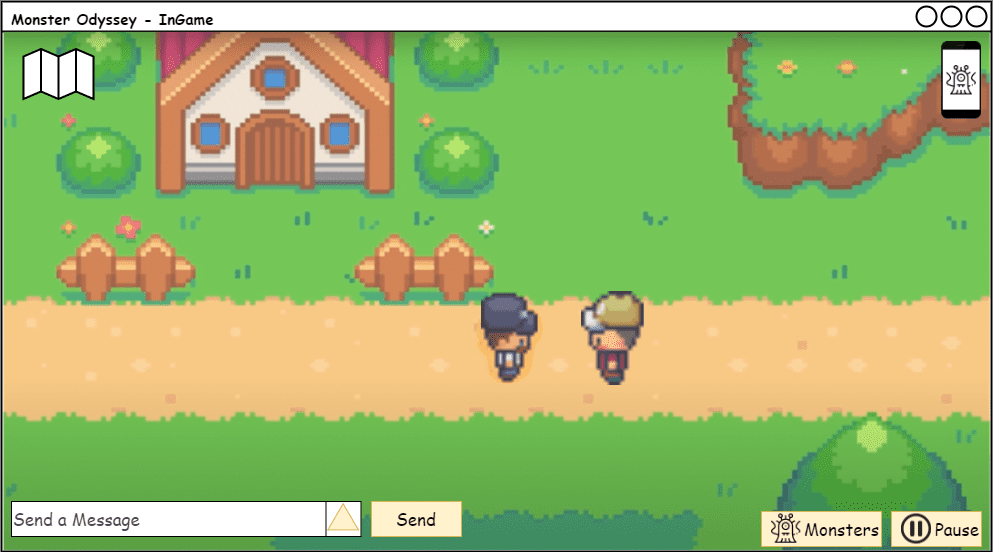
\includegraphics[width=\textwidth]{images/mockups/General/PlayerAndPlayer}
        \caption{Nutzer und NPC-Trainer voreinander}
        \label{fig: User and NPC-Trainer}
    \end{subfigure}
    \hfill
    \begin{subfigure}[b]{0.4\textwidth}
        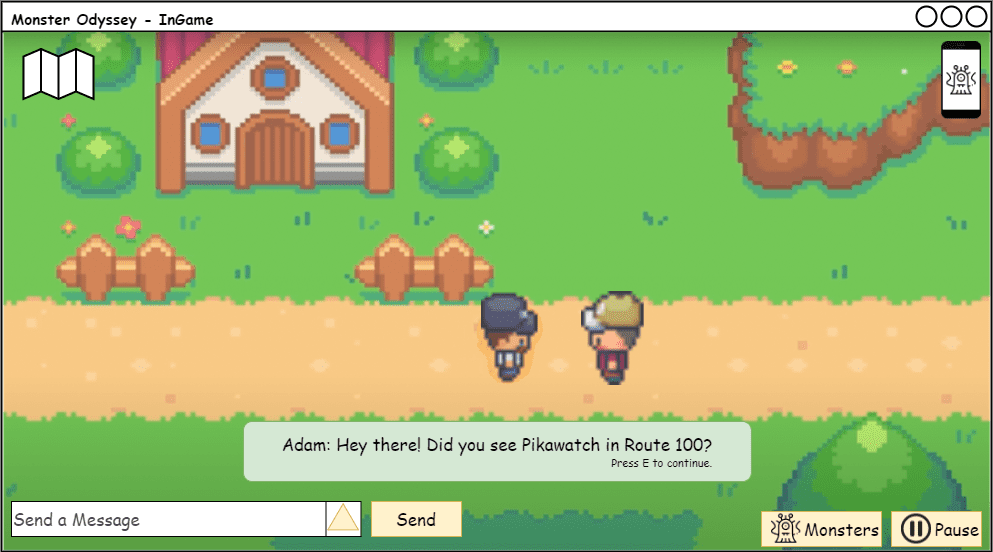
\includegraphics[width=\textwidth]{images/mockups/General/PlayerAndNPCMessage}
        \caption{Dialog zwischen Nutzer und NPC-Trainer}
        \label{fig: Dialog User and NPC-Trainer}
    \end{subfigure}
    \caption{Mockup: Starten eines Dialogs mit NPC-Trainer}
    \label{fig: Starten eines Dialogs mit NPC-Trainer}
\end{figure}
\subsection{Vergleich zwischen Mockups und Implementierung}\label{subsec:vergleich-zwischen-mockups-und-implementierung-dialogsystem}
In der Abbildung~\ref{fig: Vergleich: Anforderung Dialogsystem} sind verschiedene Unterschiede anzumerken. Bezüglich der Anforderung des Dialogsystems ist der Dialogbehälter deutlich größer als auf den Mockups wie in der Abbildung~\ref{fig: Mockup: Dialog zwischen Nutzer und NPC-Trainer}. Dies ist darauf zurückzuführen, dass einige Dialogtexte in den angebotenen Sprachen viel Platz in Anspruch nehmen. Außerdem ist die Schriftgröße der Anzeige zum Fortsetzen des Dialogs etwas größer formatiert, da dies für den Nutzer durch die Hervorhebung leichter zu identifizieren. Darüber hinaus ist der Trainername des angesprochenen Trainers in einem eigenen Behälter, über dem Dialogbehälter links liegend, vorzufinden. Somit werden der Text und der Name klar getrennt, um den Namen hervorzuheben. Der Namensbehälter wird in der Implementierung wie in der Abbildung~\ref{fig: Implementierung: Dialog zwischen Nutzer und NPC-Trainer} mit hellgrünem Hintergrund ausgestattet, damit Variabilität erzielt werden kann.

\begin{figure}[H]
    \centering
    \begin{subfigure}[b]{0.4\textwidth}
        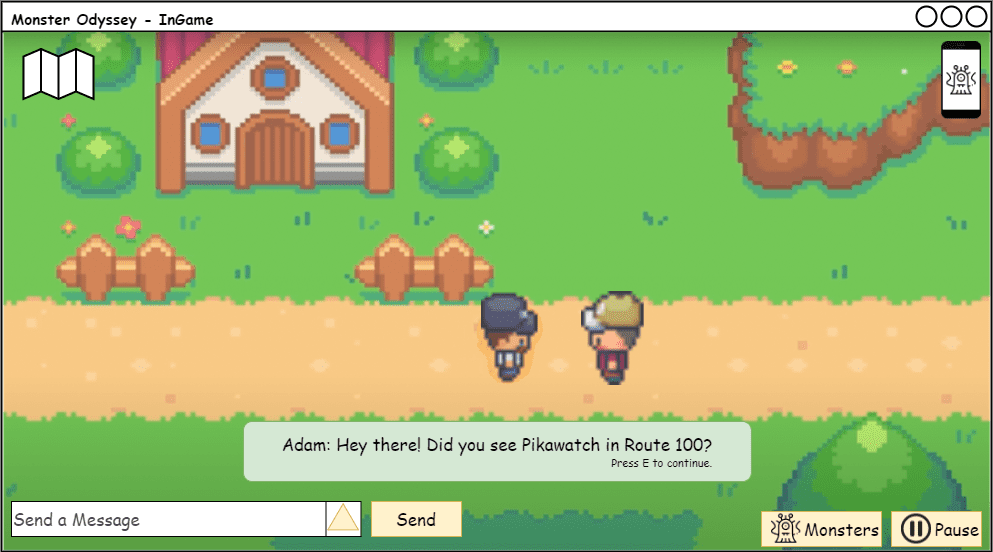
\includegraphics[width=\textwidth]{images/mockups/General/PlayerAndNPCMessage.png}
        \caption{Mockup: Dialog zwischen Nutzer und NPC-Trainer}
        \label{fig: Mockup: Dialog zwischen Nutzer und NPC-Trainer}
    \end{subfigure}
    \hfill
    \begin{subfigure}[b]{0.4\textwidth}
        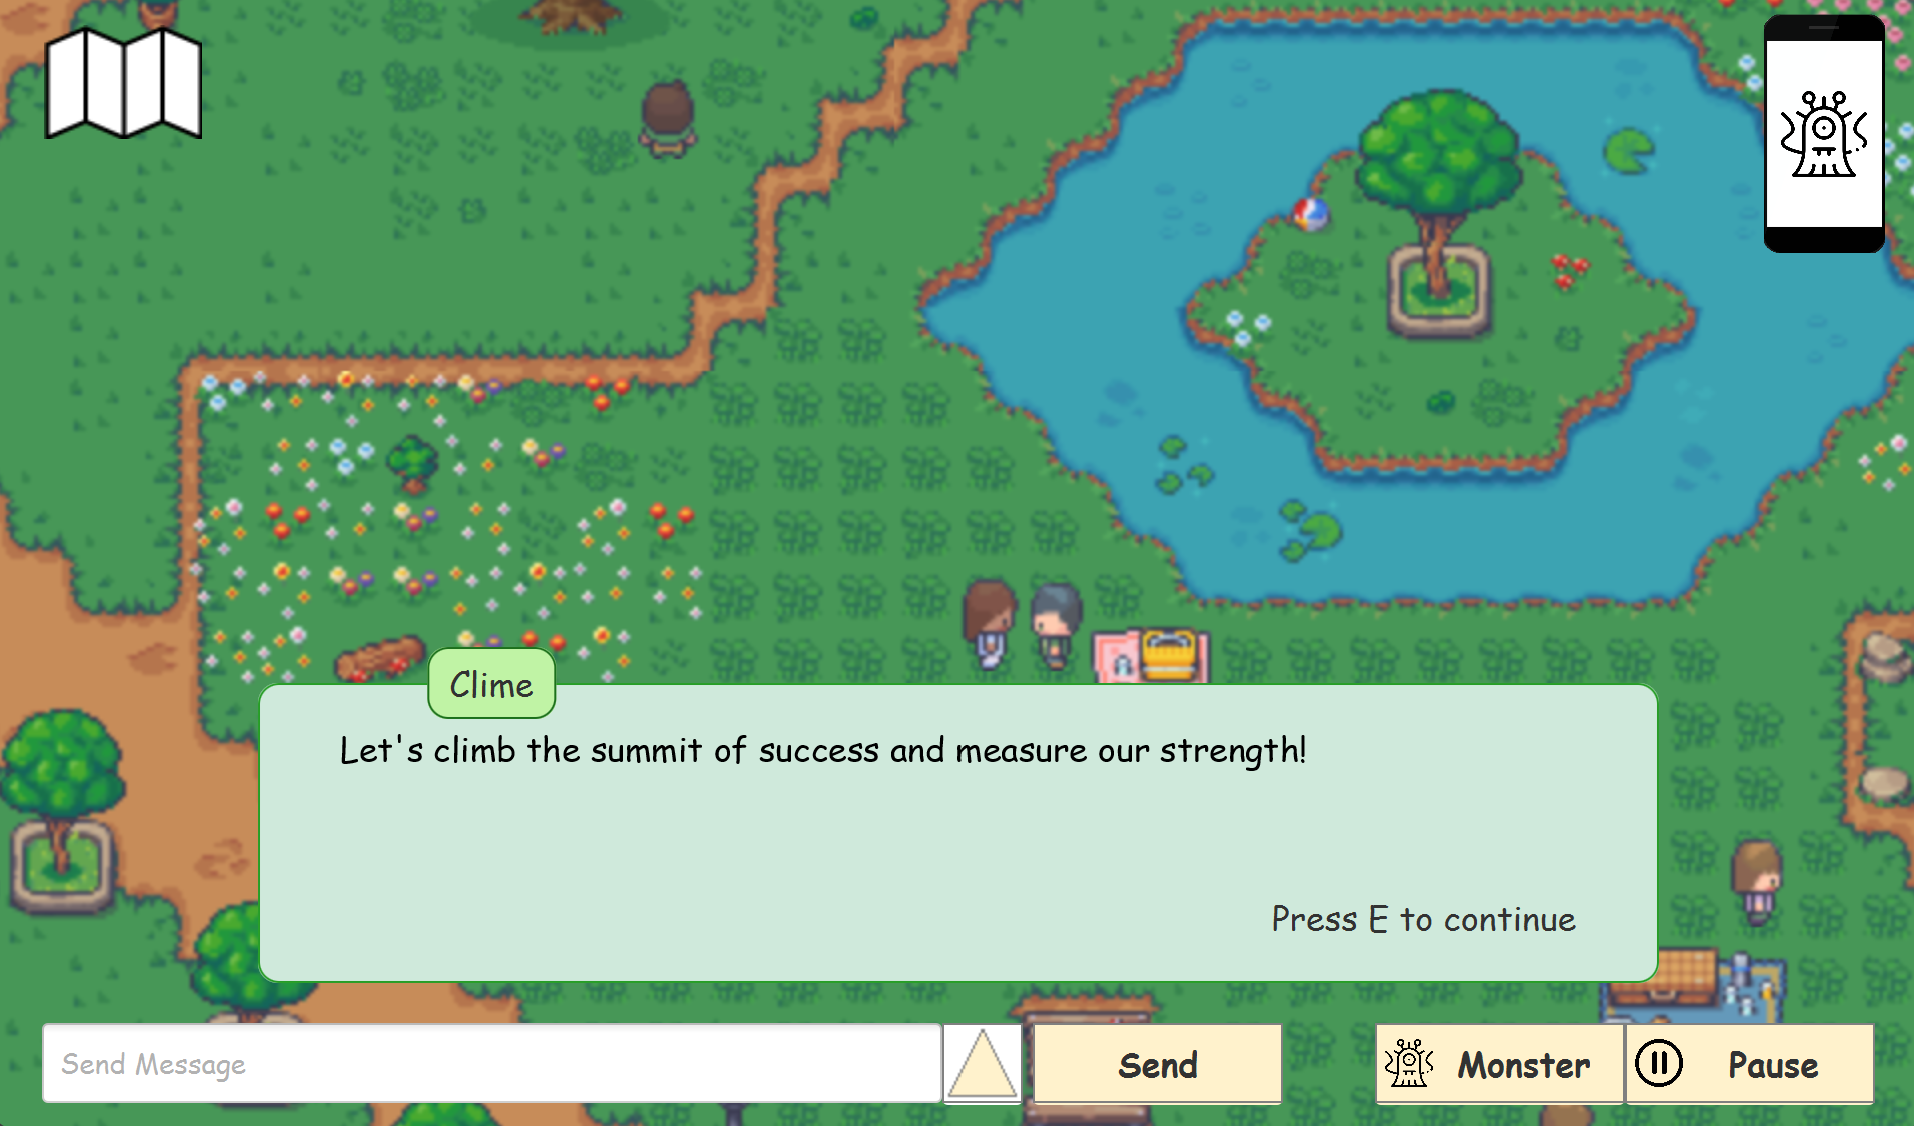
\includegraphics[width=\textwidth]{images/implementation/General/Implementierung Dialog.png}
        \caption{Implementierung: Dialog zwischen Nutzer und NPC-Trainer}
        \label{fig: Implementierung: Dialog zwischen Nutzer und NPC-Trainer}
    \end{subfigure}
    \caption{Vergleich: Anforderung Dialogsystem}
    \label{fig: Vergleich: Anforderung Dialogsystem}
\end{figure}
\section{Starter-Monster}\label{sec:starter-monster}
Der Erhalt von Monstern wird dem Nutzer anfänglich erleichtert.
In diesem Release wird der Erhalt des Starter-Monsters von dem NPC-Trainer Prof. Albert bereitgestellt, wenn der Nutzer mit ihm einen Dialog startet und eine Auswahl an Monstern trifft.
\subsection{Mockups}\label{subsec:mockups-starter-monster}
Der Nutzer steht in der Abbildung~\ref{fig: User and Prof. Albert voreinander} vor dem NPC-Trainer Prof. Albert und startet einen Dialog nach dem Drücken der Interaktionstaste.
In diesem Dialog wie in Abbildung~\ref{fig: Dialog Nutzer und Prof. Albert} heißt der NPC-Trainer Prof. Albert den Nutzer willkommen und bietet ihm verschiedene Starter-Monster an.
Diese Starter-Monster sieht der Nutzer ebenfalls nach Drücken der Interaktionstaste.  
\begin{figure}[H]
    \centering
    \begin{subfigure}[b]{0.4\textwidth}
        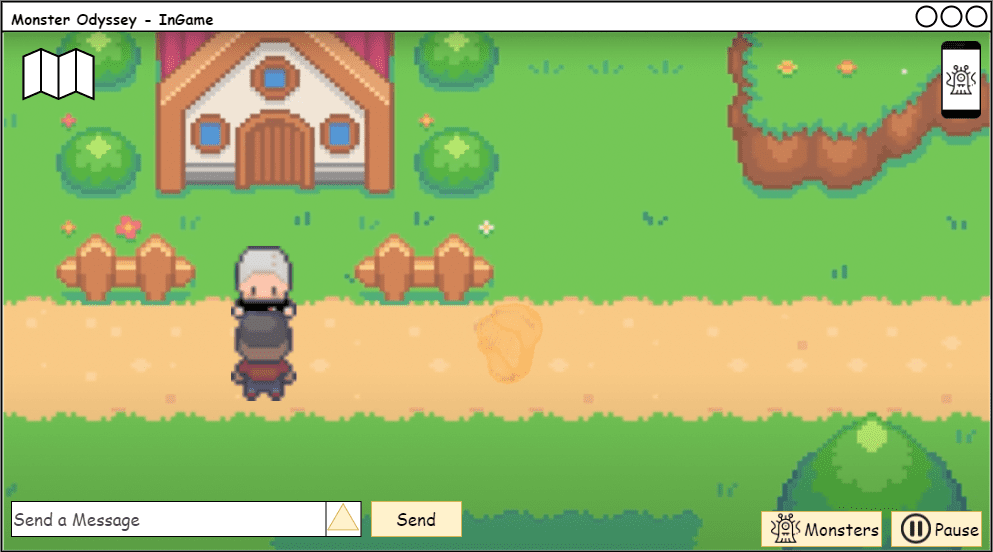
\includegraphics[width=\textwidth]{images/mockups/Starter/PlayerAndProf}
        \caption{Nutzer und Prof. Albert voreinander}
        \label{fig: User and Prof. Albert voreinander}
    \end{subfigure}
    \hfill
    \begin{subfigure}[b]{0.4\textwidth}
        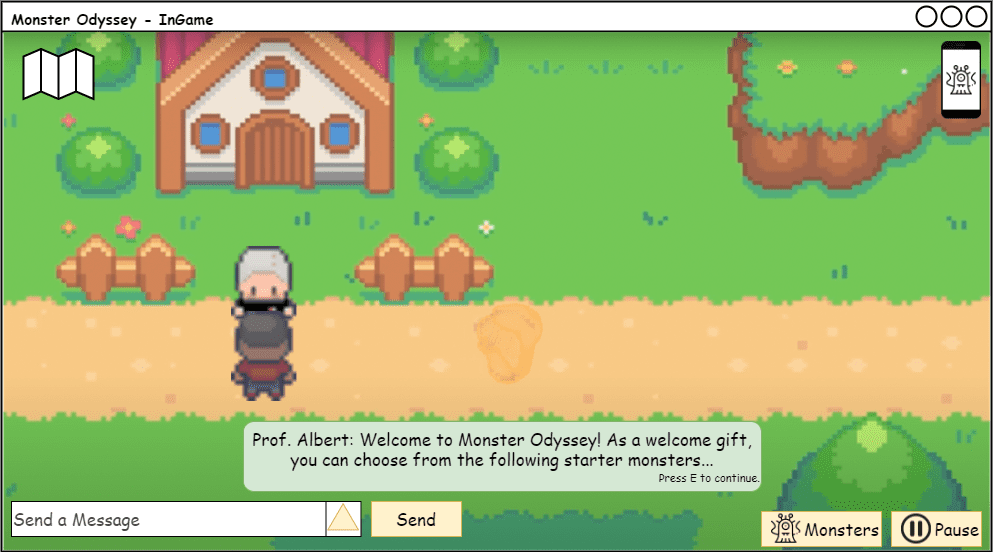
\includegraphics[width=\textwidth]{images/mockups/Starter/PlayerAndProfMessage}
        \caption{Dialog zwischen Nutzer und Prof. Albert}
        \label{fig: Dialog Nutzer und Prof. Albert}
    \end{subfigure}
    \caption{Mockup: Starten eines Dialogs mit Prof. Albert}
    \label{fig: Starten eines Dialogs mit Prof. Albert}
\end{figure}
Nachdem der Nutzer die Interaktionstaste getätigt hat, erscheint ein Popup wie in Abbildung~\ref{fig: Erste Auswahl an Starter-Monstern}, indem die Selektion des Starter-Monsters stattfindet.
Es werden drei verschiedene Monster angeboten, die von dem Server festgelegt sind.
Im Folgenden werden die Elemente nur anhand der ersten Auswahl an Starter-Monstern beschrieben.
In diesem Popup sind ein Bild, ein Monster-Typ, ein Name und eine kurze Beschreibung des jeweiligen Monsters dargestellt. Der Monster-Typ ist in einem Kästchen platziert, das farblich nach diesem Typen gekennzeichnet ist. Diese dargelegten Elemente variieren je nach dem aktuell ausgewählten Monster.
Durch die Pfeile auf der linken beziehungsweise rechten Seite des Popups kann der Nutzer zunächst zum angebotenen Starter-Monster wechseln und seine zugehörigen Elemente sehen.
\begin{figure}[H]
    \center
    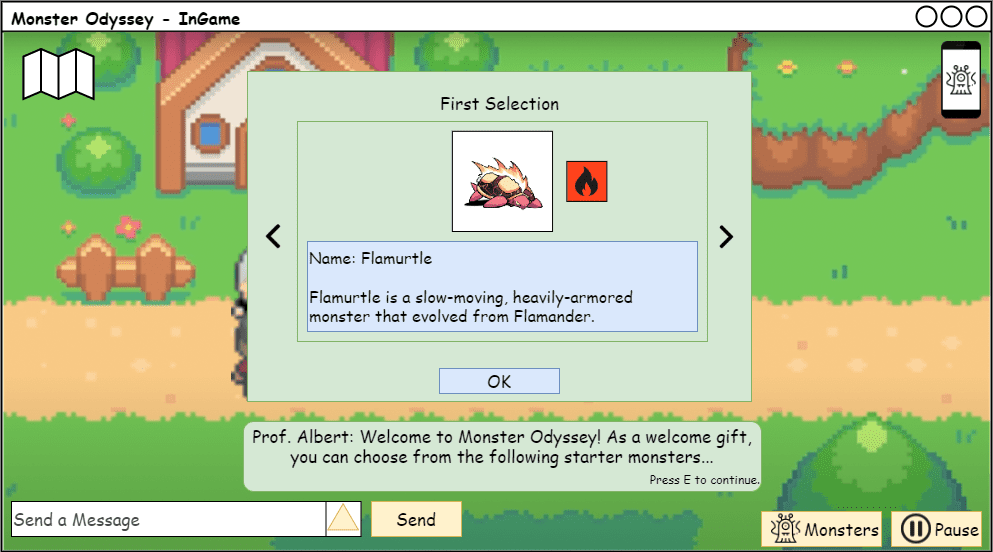
\includegraphics[scale=\scale]{images/mockups/Starter/PlayerAndProfMonsterSelection}
    \caption{Mockup: Erste Auswahl an Starter-Monstern}
    \label{fig: Erste Auswahl an Starter-Monstern}
\end{figure}
Entscheidet sich der Nutzer für ein Starter-Monster, so kann er mit dem 'OK'-Knopf auf dem Popup aus Abbildung~\ref{fig: Erste Auswahl an Starter-Monstern} seine Auswahl bestätigen.  Somit erhält der Nutzer das ausgewählte Starter-Monster und dieses wird zu der Monsterliste des Nutzers hinzugefügt. Dabei erscheint erneut ein Popup, wie in Abbildung~\ref{fig: Erhaltener Starter-Monster}, mit den Elementen des Monsters, zusätzlich erscheint eine Beschriftung, dass das Monster hinzugefügt wurde.
Beim Drücken des 'OK'-Knopfs wird der Dialog fortgesetzt, in dem der NPC-Trainer Prof. Albert dem Nutzer viel Erfolg wünscht. Der Dialog kann beendet werden, wenn der Nutzer in der Spielsituation wie in der Abbildung~\ref{fig: Nach Erhalt des Starter-Monsters} die Interaktionstaste tätigt.
\begin{figure}[H]
    \center
    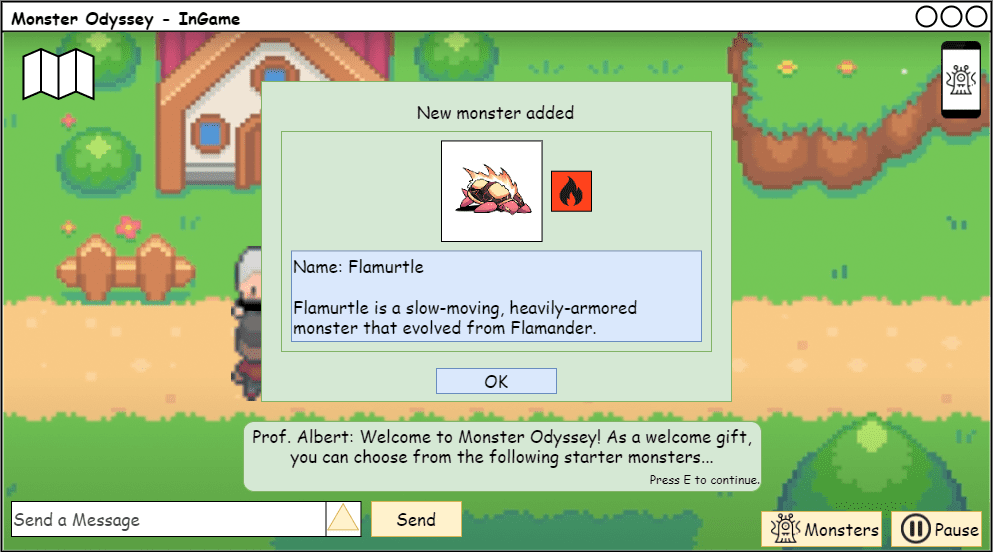
\includegraphics[scale=\scale]{images/mockups/Starter/PlayerAndProfMonsterReceived}
    \caption{Mockup: Erhaltener Starter-Monster}
    \label{fig: Erhaltener Starter-Monster}
\end{figure}
\begin{figure}[H]
    \center
    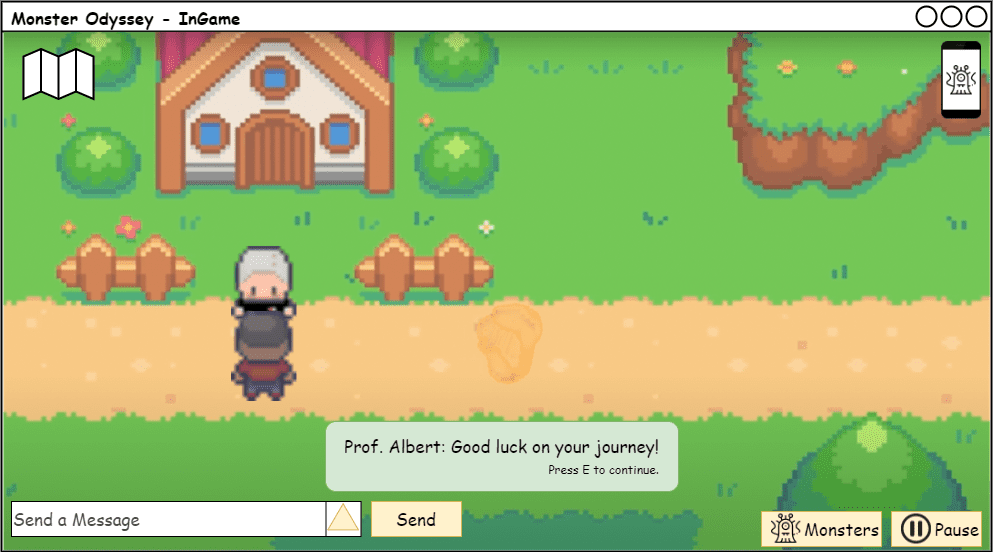
\includegraphics[scale=\scale]{images/mockups/Starter/PlayerAndProfAfterReceived}
    \caption{Mockup: Nach Erhalt des Starter-Monsters}
    \label{fig: Nach Erhalt des Starter-Monsters}
\end{figure}
Falls der Nutzer bereits ein Starter-Monster von dem NPC-Trainer Prof. Albert erhalten hat, so wird der Nutzer beim Interagieren mit ihm einen Dialog starten, aber keine neuen Starter-Monster bekommen können. Dabei weist Prof. Albert den Nutzer wie in Abbildung~\ref{fig: Starter-Monster bereits erhalten} darauf hin, dass er bereits dem Nutzer ein Starter-Monster überreicht hatte.
\begin{figure}[H]
    \center
    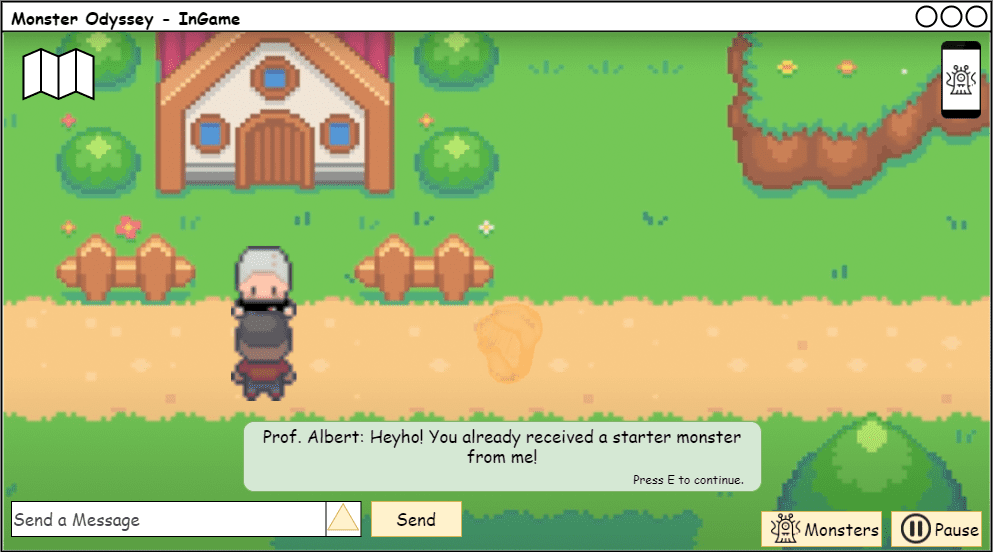
\includegraphics[scale=\scale]{images/mockups/Starter/PlayerAndProfAlreadyReceived}
    \caption{Mockup: Starter-Monster bereits erhalten}
    \label{fig: Starter-Monster bereits erhalten}
\end{figure}
\subsection{Vergleich zwischen Mockups und Implementierung}\label{subsec:vergleich-zwischen-mockups-und-implementierung-starter-monster}
In der Abbildung~\ref{fig: Vergleich: Starten eines Dialogs mit Prof. Albert} sind die Elemente des Dialogsystems verschieden, was in Abschnitt~\ref{subsec:vergleich-zwischen-mockups-und-implementierung-dialogsystem} angedeutet wurde. Auch die Dialogtexte variieren, um in der Implementierung ansprechendere und humoristische Dialogtexte zu formulieren, damit das Spielerlebnis unterhaltsam gestaltet wird.
\begin{figure}[H]
    \centering
    \begin{subfigure}[b]{0.4\textwidth}
        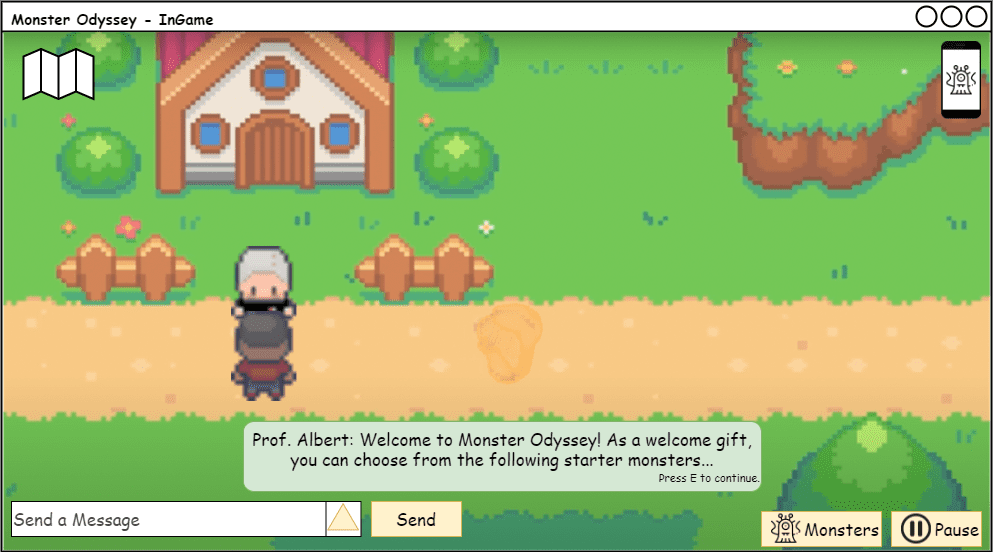
\includegraphics[width=\textwidth]{images/mockups/Starter/PlayerAndProfMessage}
        \caption{Mockup: Dialog zwischen Nutzer und Prof. Albert}
        \label{fig: Mockup: Dialog Nutzer und Prof. Albert}
    \end{subfigure}
    \hfill
    \begin{subfigure}[b]{0.4\textwidth}
        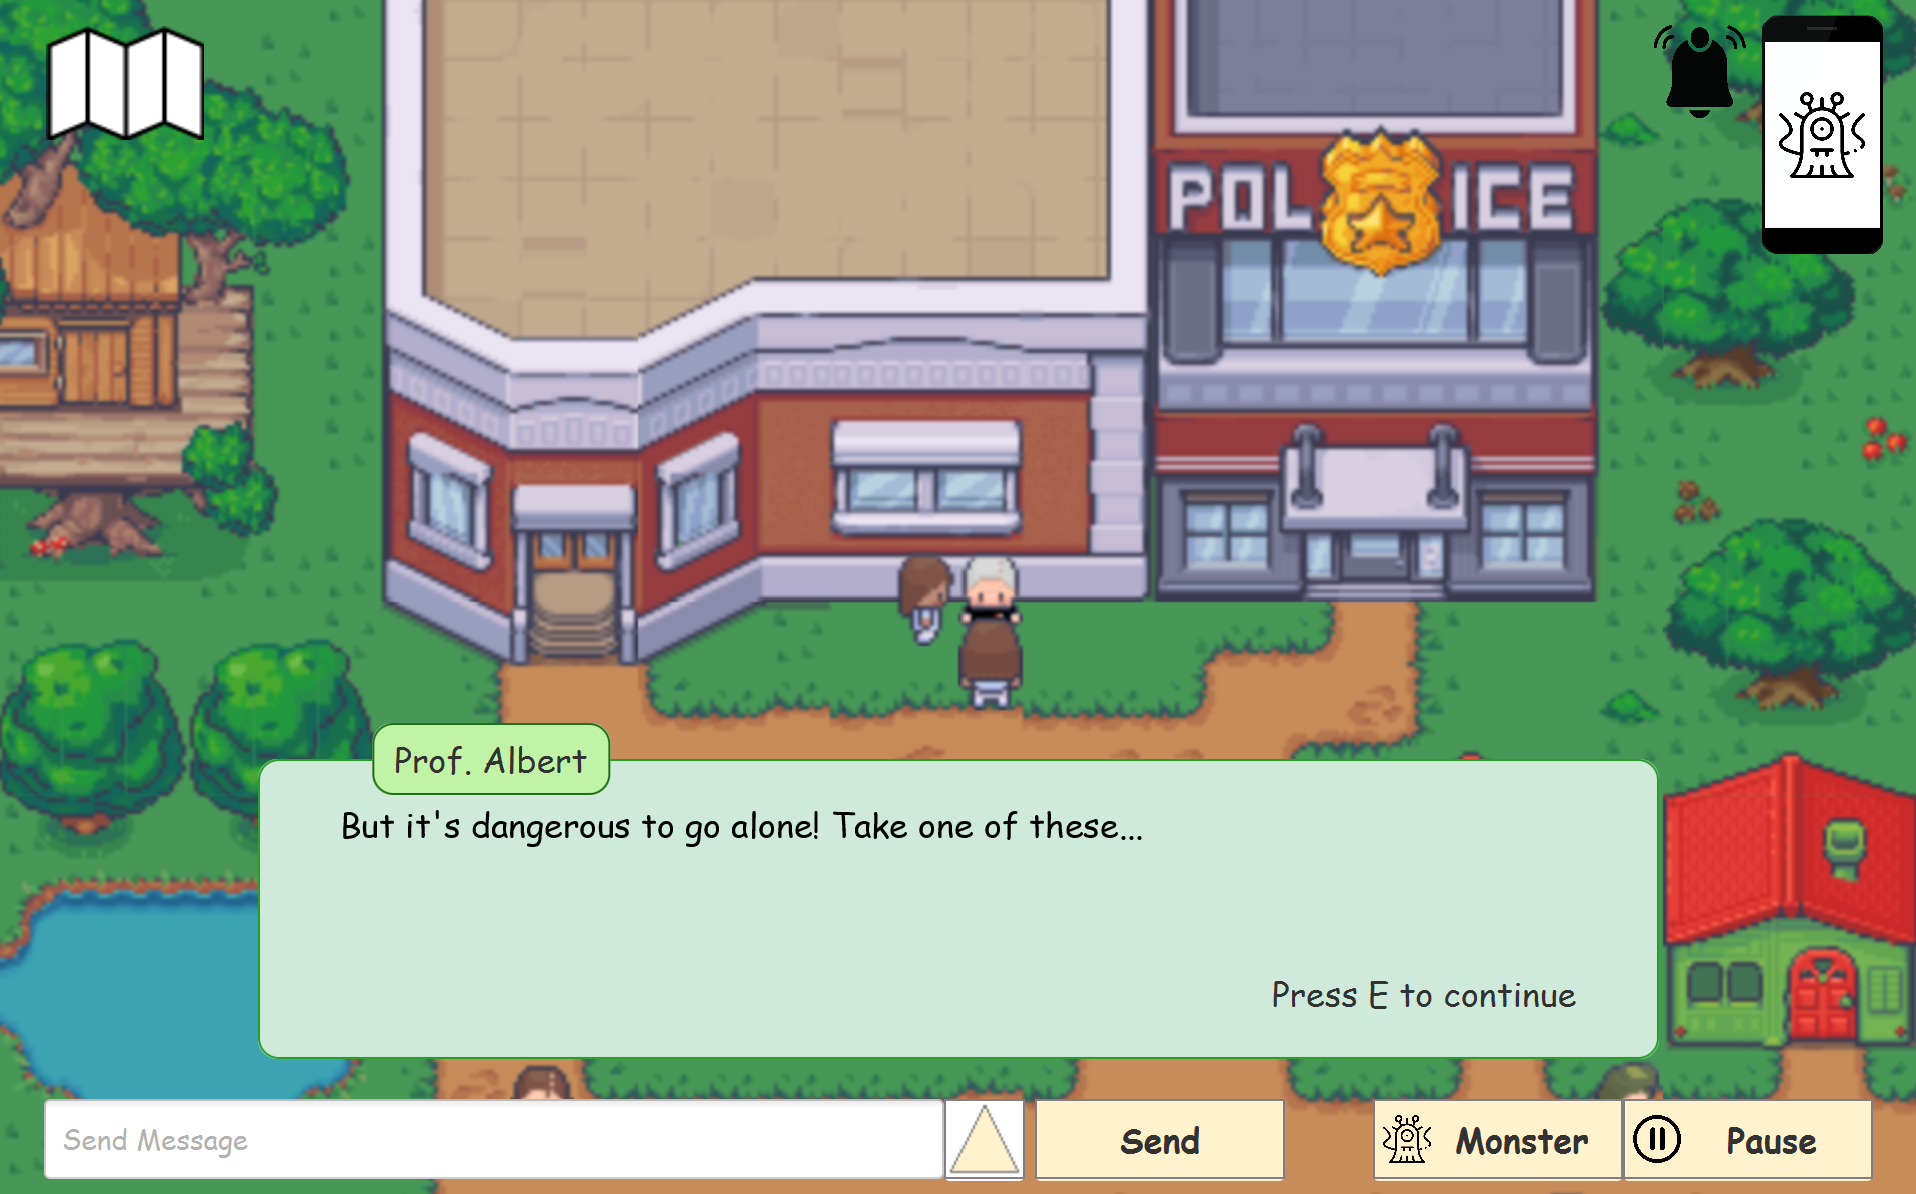
\includegraphics[width=\textwidth]{images/implementation/Starter/Implement dialog.png}
        \caption{Implementierung: Dialog zwischen Nutzer und Prof. Albert}
        \label{fig: Implementierung: Dialog Nutzer und Prof. Albert}
    \end{subfigure}
    \caption{Vergleich: Starten eines Dialogs mit Prof. Albert}
    \label{fig: Vergleich: Starten eines Dialogs mit Prof. Albert}
\end{figure}
Darüber hinaus ist in der Abbildung~\ref{fig: Vergleich: Auswahl an Starter-Monsters} zu sehen, dass die Elemente in den Mockups mit den Elementen in der Implementierung identisch sind, wobei die Starter-Monster verschieden sind. Der Hintergrund erhält einen Unschärfeeffekt, um dadurch die Konzentration des Nutzers auf die Auswahl an Starter-Monster zu lenken.

In der Abbildung~\ref{fig: Vergleich: Erhaltener Starter-Monster} ist zu bemerken, dass die Elemente, abgesehen von den Unterschieden aus den vorherigen Abbildungen, übereinstimmend sind. 
\begin{figure}[H]
    \centering
    \begin{subfigure}[b]{0.4\textwidth}
        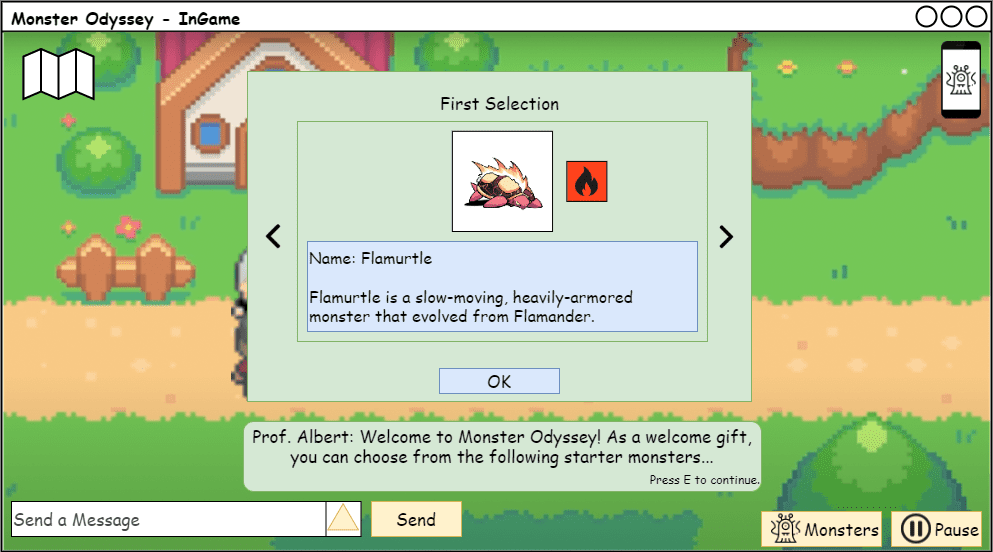
\includegraphics[width=\textwidth]{images/mockups/Starter/PlayerAndProfMonsterSelection}
        \caption{Mockup: Erste Auswahl an Starter-Monstern}
        \label{fig: Mockup: Erste Auswahl an Starter-Monstern}
    \end{subfigure}
    \hfill
    \begin{subfigure}[b]{0.4\textwidth}
        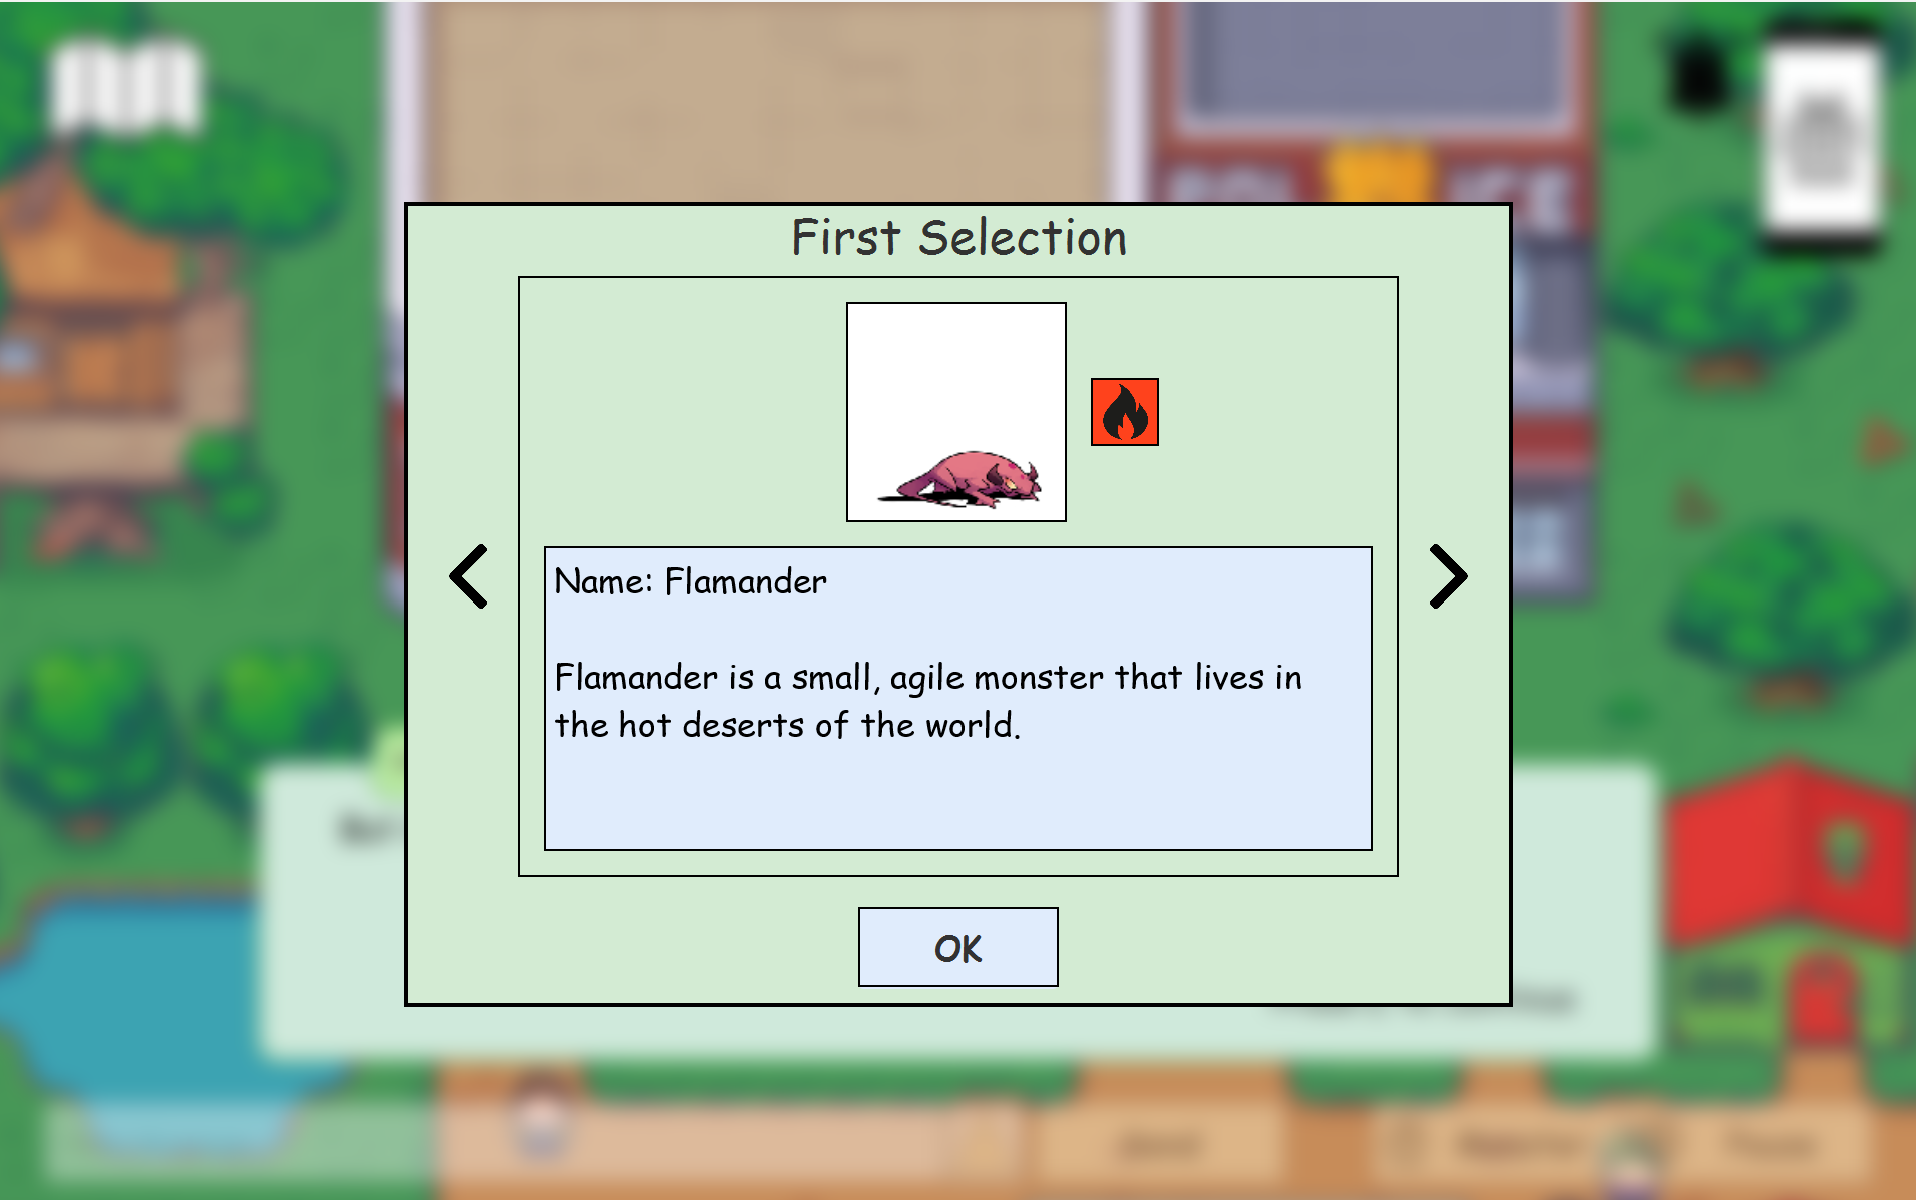
\includegraphics[width=\textwidth]{images/implementation/Starter/Starter selection implementation.png}
        \caption{Implementierung: Erste Auswahl an Starter-Monstern}
        \label{fig: Implementierung: Erste Auswahl an Starter-Monstern}
    \end{subfigure}
    \caption{Vergleich: Auswahl an Starter-Monsters}
    \label{fig: Vergleich: Auswahl an Starter-Monsters}
\end{figure}
\begin{figure}[H]
    \centering
    \begin{subfigure}[b]{0.4\textwidth}
        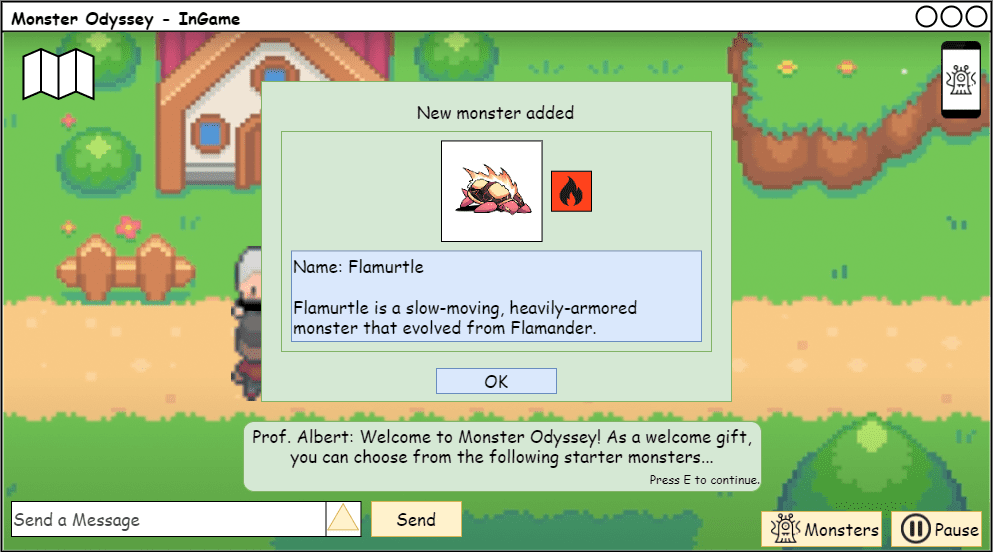
\includegraphics[width=\textwidth]{images/mockups/Starter/PlayerAndProfMonsterReceived}
        \caption{Mockup: Erhalt des Starter-Monsters}
        \label{fig: Mockup: Erhaltener Starter-Monster}
    \end{subfigure}
    \hfill
    \begin{subfigure}[b]{0.4\textwidth}
        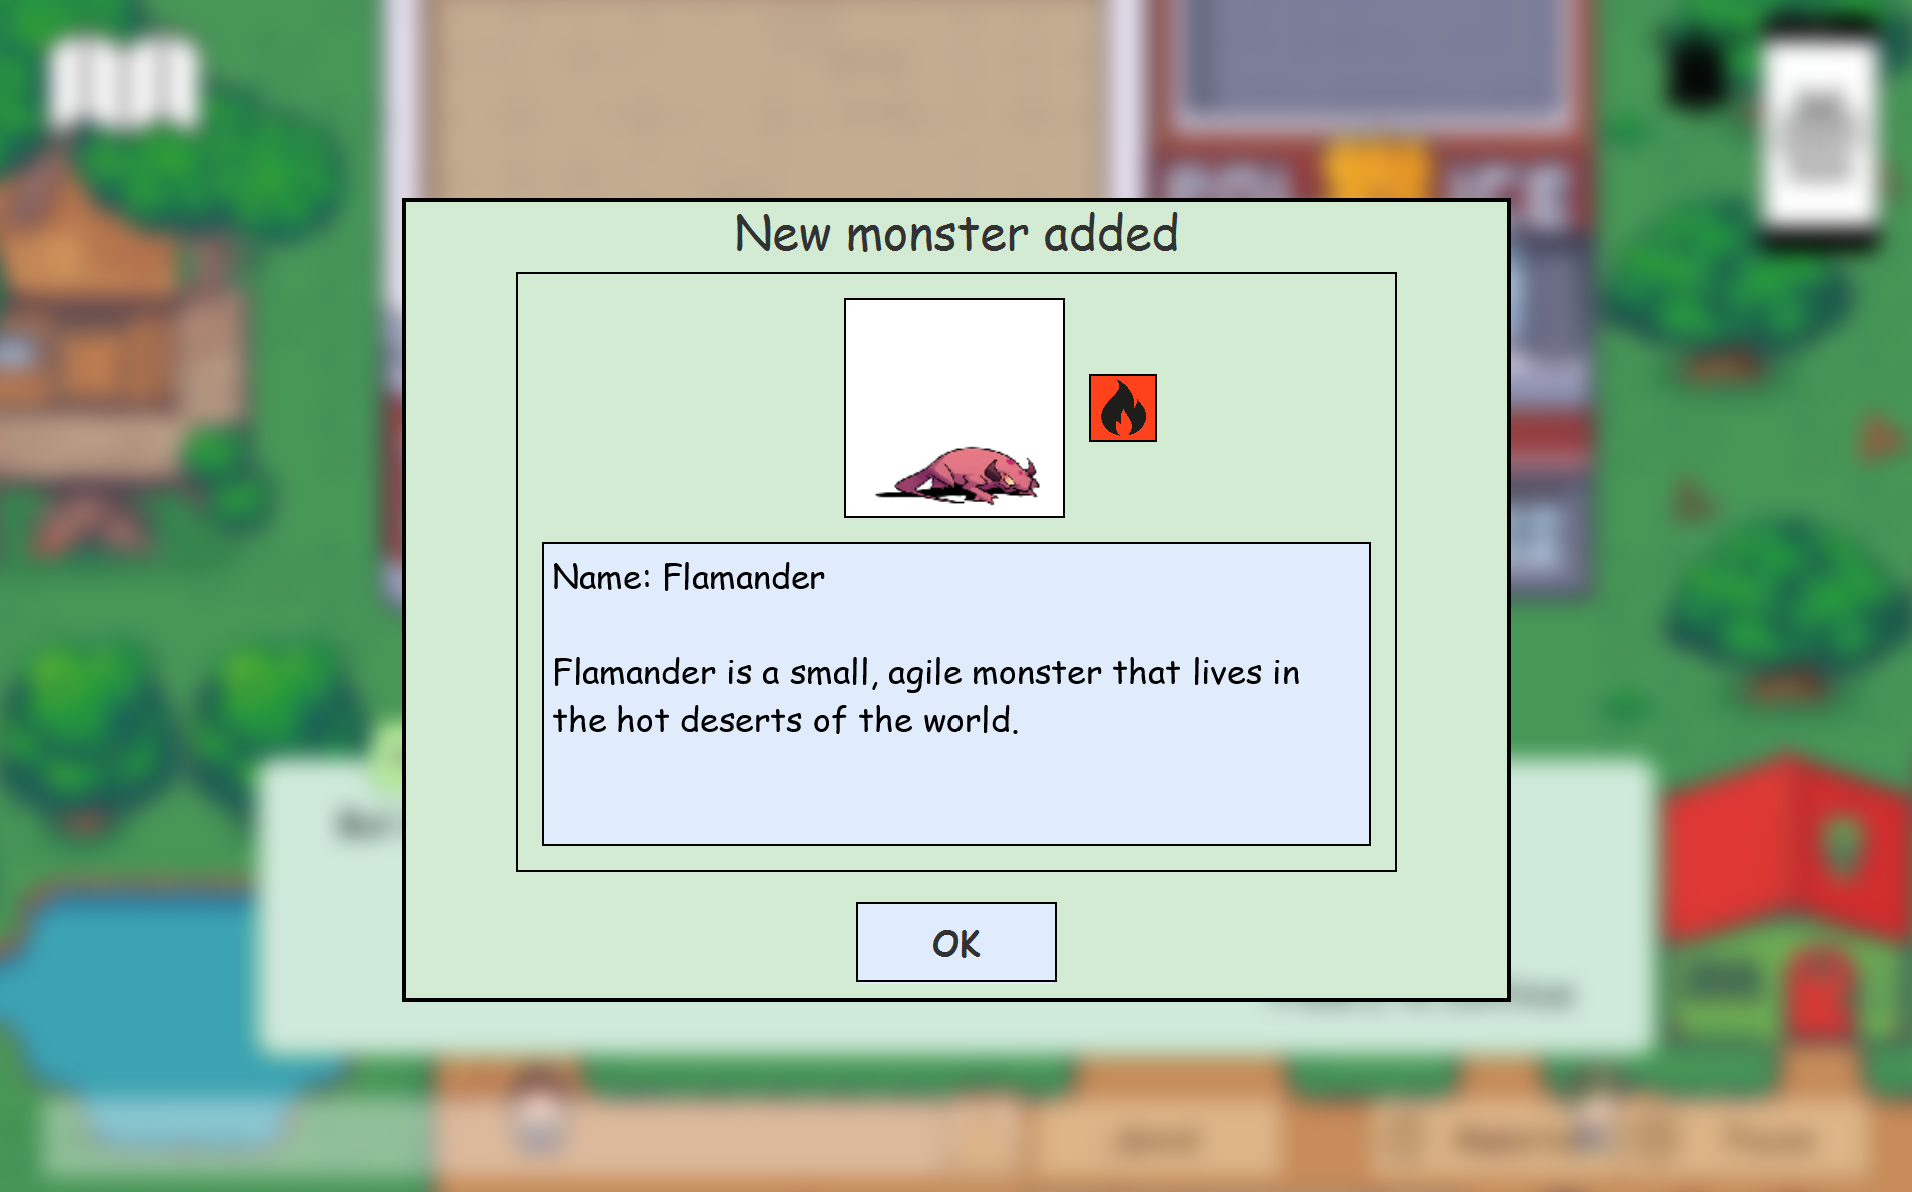
\includegraphics[width=\textwidth]{images/implementation/Starter/New Monster added implementation.png}
        \caption{Implementierung: Erhalt des Starter-Monsters}
        \label{fig: Implementierung: Erhaltener Starter-Monster}
    \end{subfigure}
    \caption{Vergleich: Erhalt des Starter-Monsters}
    \label{fig: Vergleich: Erhaltener Starter-Monster}
\end{figure}
\section{Kampf starten}\label{sec:kampf-starten}
Nachdem der Nutzer das Starter-Monster erhalten hat, kann er Kämpfe mit anderen (NPC-)Trainern und wilden Monstern starten. Hier ist wichtig zu beachten, dass nur einige NPC-Trainer das Attribut haben, mit dem Nutzer kämpfen zu können.
\subsection{Mockups}\label{subsec:mockups-kampf-starten}
Es gibt mehrere Möglichkeiten zum Start eines Kampfes.
Der Nutzer kann beispielsweise einen anderen Trainer ansprechen und damit einen Kampf mit dem Trainer hervorrufen. Dabei wird im Falle eines NPC-Trainers ein Dialog eröffnet, in dem der NPC-Trainer den Nutzer wie in der Abbildung~\ref{fig: Dialog zwischen Nutzer und NPC-Trainer für Kampf} herausfordert.
Ansonsten wird beim Sprechen mit einem anderen Trainer nur die Ankündigung wie in Abbildung~\ref{fig: Ankündigung über Start des Kampfs} angezeigt, dass der Start des Kampfs in Kürze gestartet wird.
Dabei sieht außerdem der Nutzer den Namen des angesprochenen Trainers.
Darüber hinaus kann ein NPC-Trainer beim Erblicken eines Nutzers versuchen, einen Kampf mit dem Nutzer zu starten. In diesem Fall wird dem Nutzer auch die Ankündigung aus der Abbildung~\ref{fig: Ankündigung über Start des Kampfs} angezeigt.
Beim Drücken der Interaktionstaste gelangt der Nutzer in die Kampfszene wie in Abschnitt~\ref{sec:kampf-führen}.
\begin{figure}[H]
    \center
    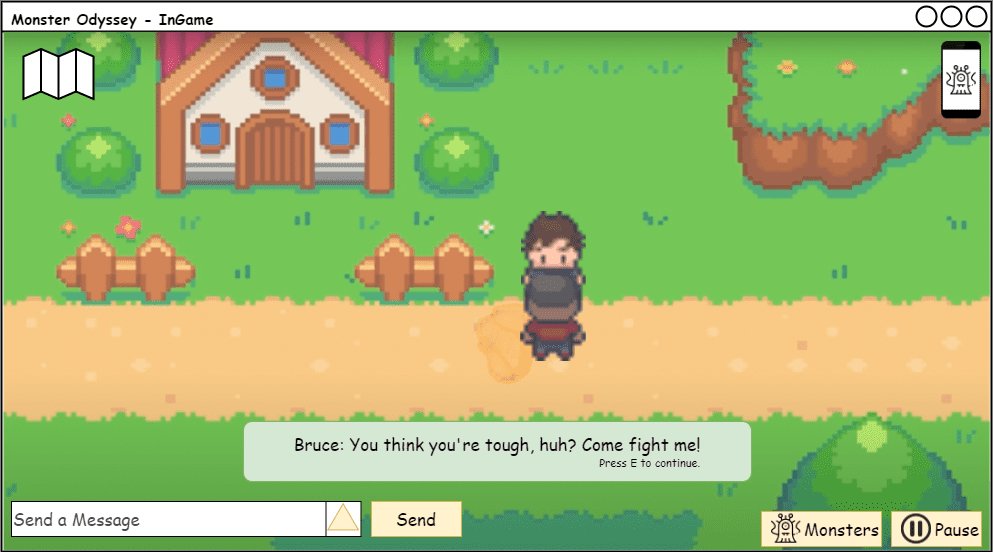
\includegraphics[scale=\scale]{images/mockups/Ingame/PlayerAndNPCStartFight.png}
    \caption{Mockup: Dialog zwischen Nutzer und NPC-Trainer für Kampf}
    \label{fig: Dialog zwischen Nutzer und NPC-Trainer für Kampf}
\end{figure}
\begin{figure}[H]
    \center
    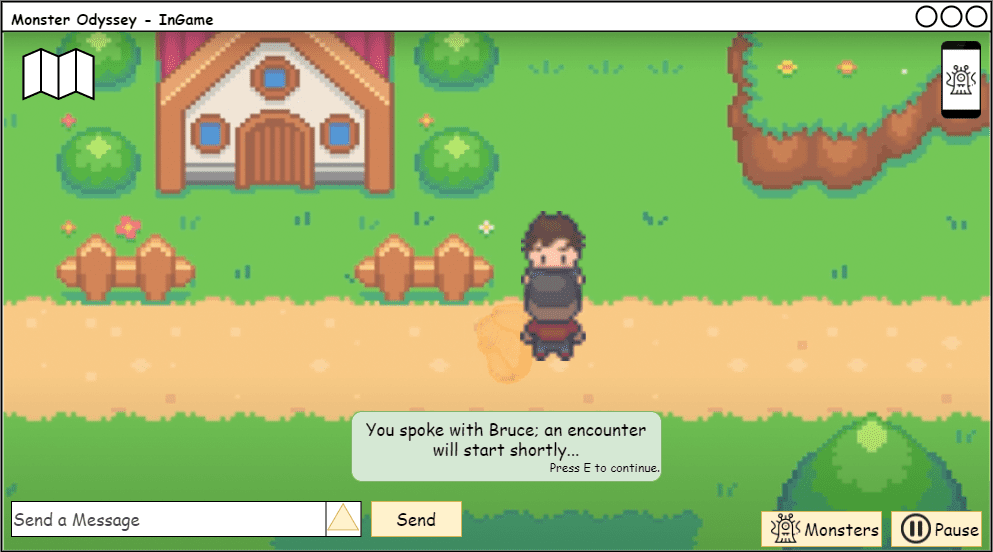
\includegraphics[scale=\scale]{images/mockups/Ingame/PlayerAndPlayerFight.png}
    \caption{Mockup: Ankündigung über Start des Kampfs}
    \label{fig: Ankündigung über Start des Kampfs}
\end{figure}
Außerdem könnte der Nutzer im hohen Gras wilden Monstern begegnen.
Der Kampfstart kommt in diesem Fall nicht von dem Nutzer aus, sondern wird von der Umgebung getroffen.
Um immer noch die Benutzerfreundlichkeit anbieten zu können, wird ebenfalls eine Ankündigung wie in der Abbildung~\ref{fig: Wildem Monster in hohem Gras begegnet} dargestellt.
Gleichermaßen gelangt der Nutzer auch hier beim Drücken der Interaktionstaste in die Kampfszene wie in Abschnitt~\ref{sec:kampf-führen}.
\begin{figure}[H]
    \center
    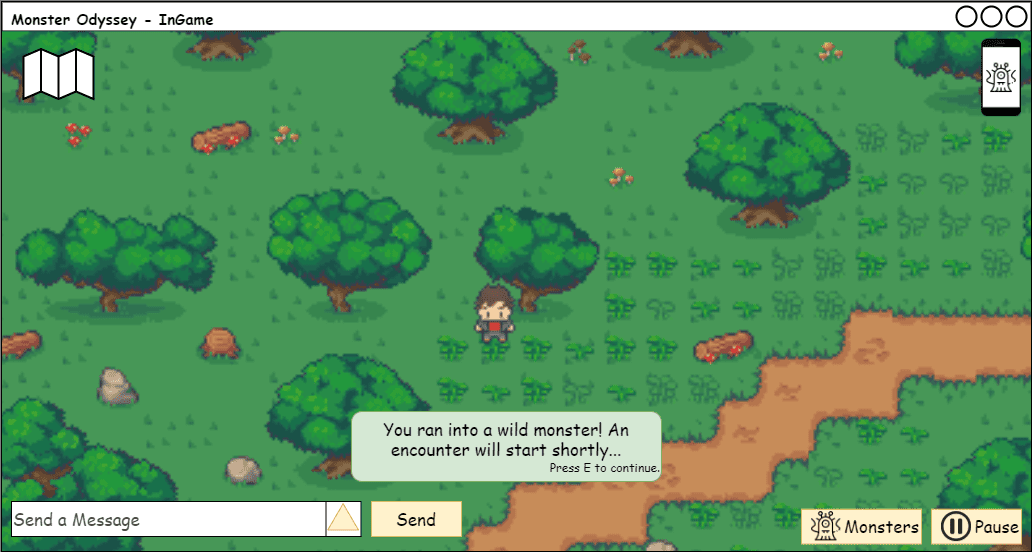
\includegraphics[scale=\scale]{images/mockups/Ingame/PlayerAndWildMonsterFight.png}
    \caption{Mockup: Wildem Monster in hohem Gras begegnet}
    \label{fig: Wildem Monster in hohem Gras begegnet}
\end{figure}
\subsection{Vergleich zwischen Mockups und Implementierung}\label{subsec:vergleich-zwischen-mockups-und-implementierung-kampf-starten}
Vor dem Kampfstart ist in der Implementierung die Ankündigung anders gestaltet. Es wird wie in Abbildung~\ref{fig: Implementierung: Ankündigung über Kampfstart} ein Dialog vor dem Kampfstart geführt, in dem der Sprechende 'Announcement' für die Ankündigung zuständig ist und der Dialogtext wie in der Abbildung~\ref{fig: Mockup: Ankündigung über Kampfstart} ohne den Namen des gegnerischen Trainers festgesetzt ist. Analog gilt es für den Kampf gegen ein wildes Monster. Das Implementieren eines Trainernamens gestaltete sich für die Entwickler schwieriger als erwartet, weshalb der Name weggelassen worden ist.

\begin{figure}[H]
    \centering
    \begin{subfigure}[b]{0.4\textwidth}
        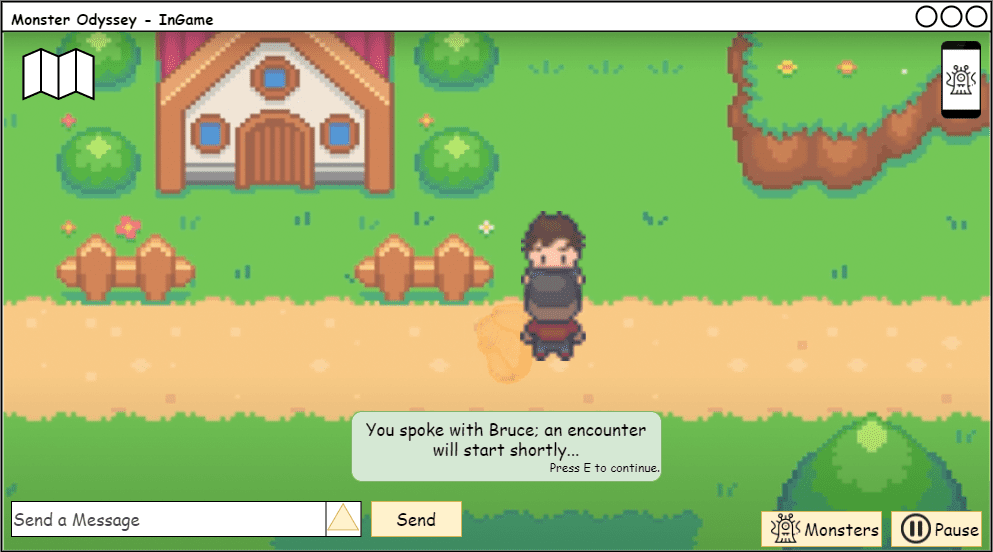
\includegraphics[width=\textwidth]{images/mockups/Ingame/PlayerAndPlayerFight.png}
        \caption{Mockup: Ankündigung über Kampfstart}
        \label{fig: Mockup: Ankündigung über Kampfstart}
    \end{subfigure}
    \hfill
    \begin{subfigure}[b]{0.4\textwidth}
        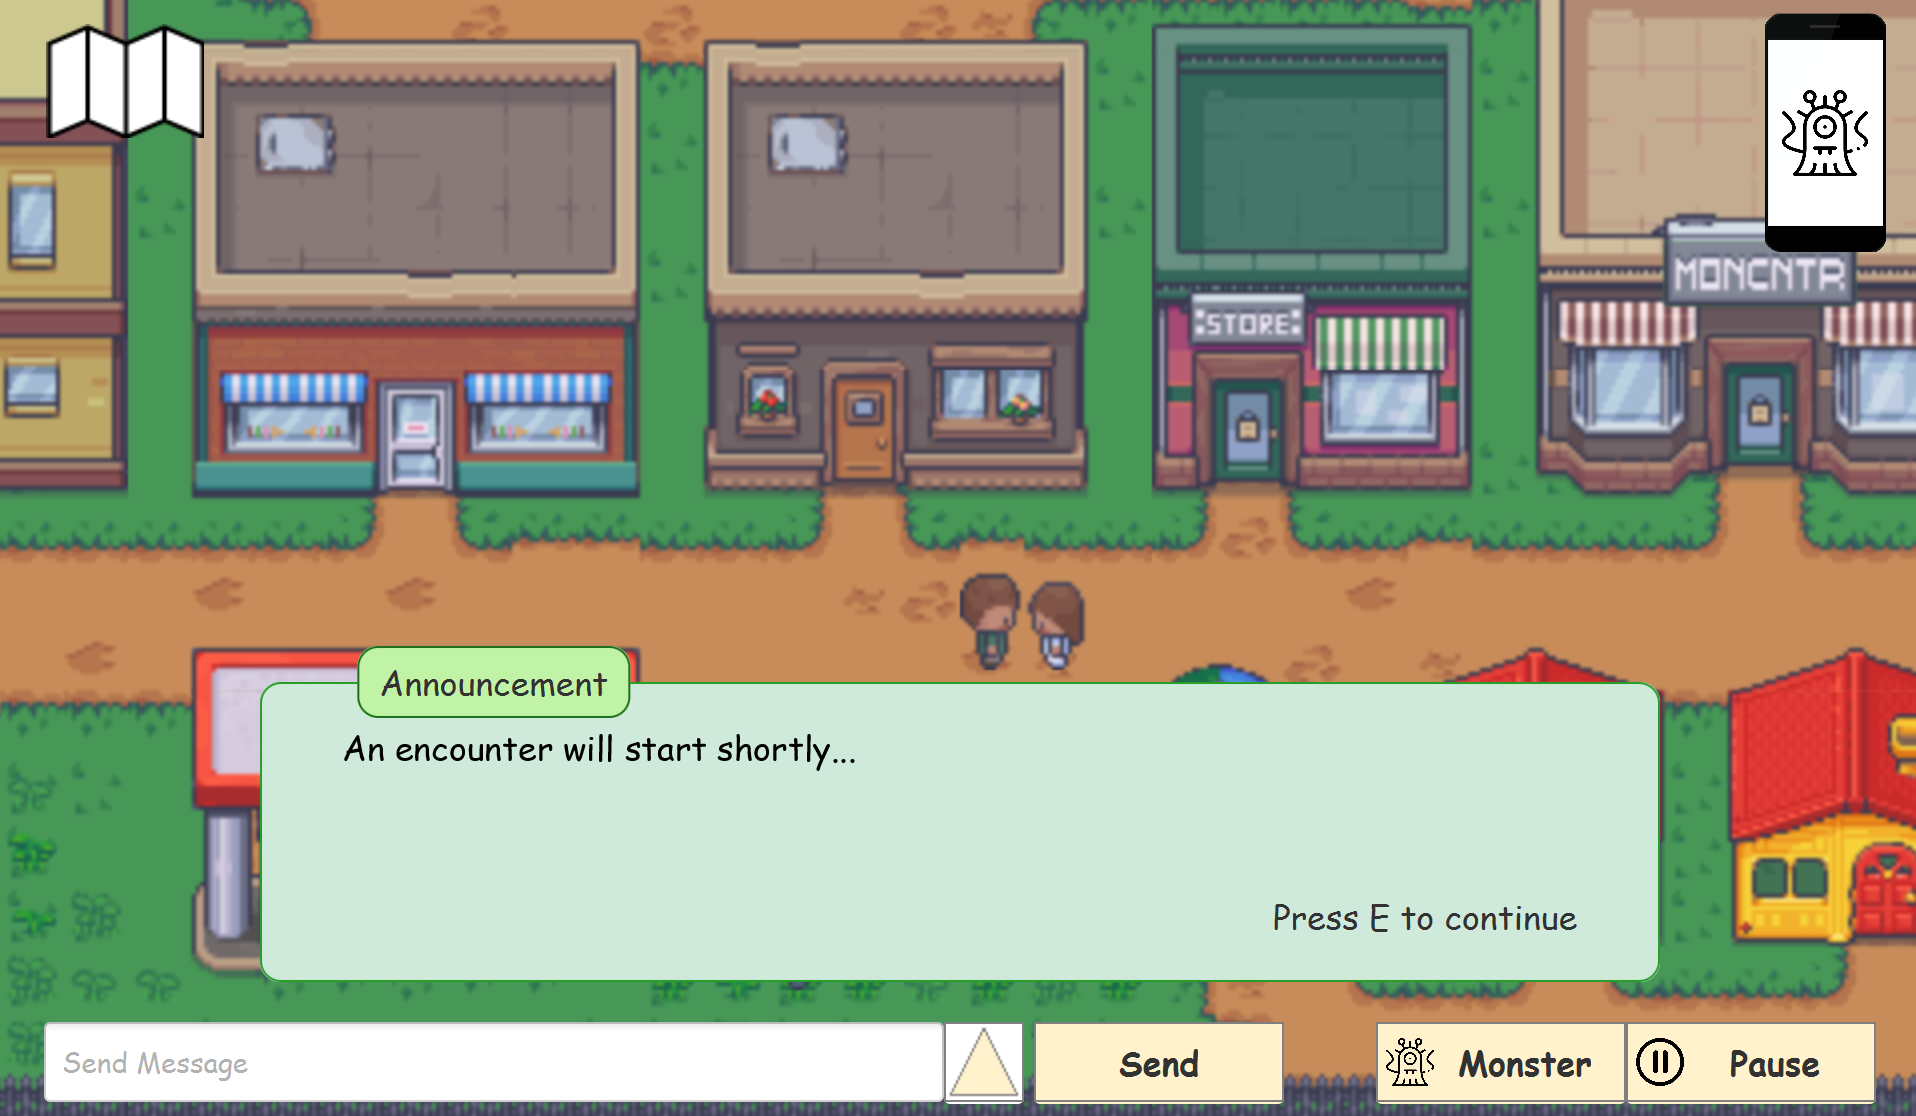
\includegraphics[width=\textwidth]{images/implementation/Ingame/Implementierung anncouncement.png}
        \caption{Implementierung: Ankündigung über Kampfstart}
        \label{fig: Implementierung: Ankündigung über Kampfstart}
    \end{subfigure}
    \caption{Vergleich: Anforderung Kampfstart}
    \label{fig: Vergleich: Anforderung Kampfstart}
\end{figure}
\section{Monsterheilung}\label{sec:monster-heilen}
Sobald der Nutzer in den Kampf einsteigt und mit seinen Monstern Angriffe startet, besteht immer die Chance, dass die Monster Leben verlieren und somit nicht die maximale Fähigkeit besitzen, optimal kämpfen zu können. Um die Monster gesund zu halten, wird es dem Nutzer ermöglicht, seine Monster zu heilen.
Die Heilungsmaßnahmen erfolgen bei einer Krankenschwester in einem 'Moncenter'.
\subsection{Mockups}\label{subsec:mockups-monster-heilen}
Jede Krankenschwester befindet sich in einem 'Moncenter' und der Nutzer kann sich jederzeit dorthin begeben.
Wenn der Nutzer einen Dialog mit der Krankenschwester startet, grüßt ihn die Krankenschwester zunächst und fragt ihn, ob er seine Monster wie in Abbildung~\ref{fig: Dialog zwischen Nutzer und Krankenschwester} heilen möchte.
Beim Drücken der Interaktionstaste wird ein Popup wie in Abbildung~\ref{fig: Heilungsfenster} geöffnet, in dem der Nutzer nochmals gefragt wird, ob er seine Monster wirklich heilen möchte.
\begin{figure}[H]
    \centering
    \begin{subfigure}[b]{0.4\textwidth}
        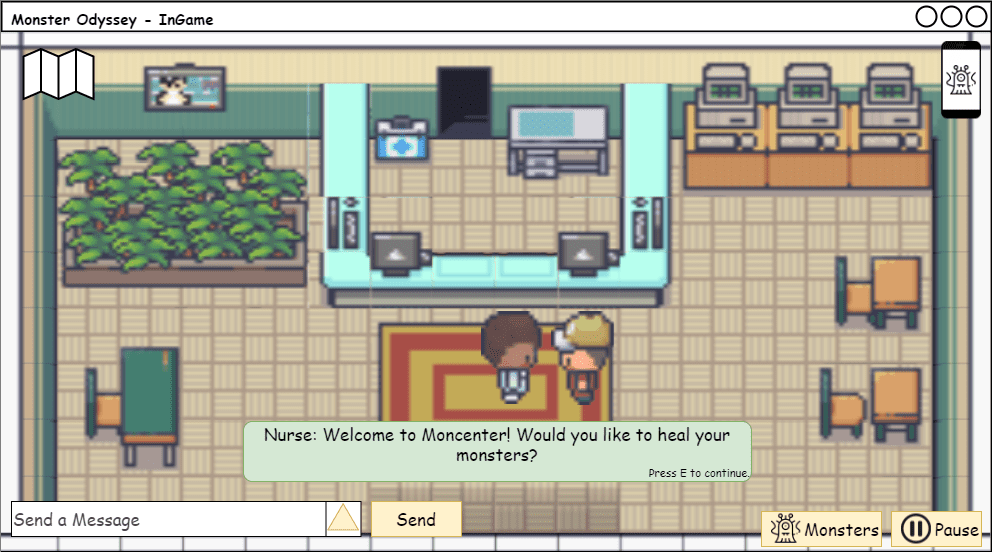
\includegraphics[width=\textwidth]{images/mockups/Heilung/PlayerInMoncenterHealingDialog.png}
        \caption{Dialog zwischen Nutzer und Krankenschwester}
        \label{fig: Dialog zwischen Nutzer und Krankenschwester}
    \end{subfigure}
    \hfill
    \begin{subfigure}[b]{0.4\textwidth}
        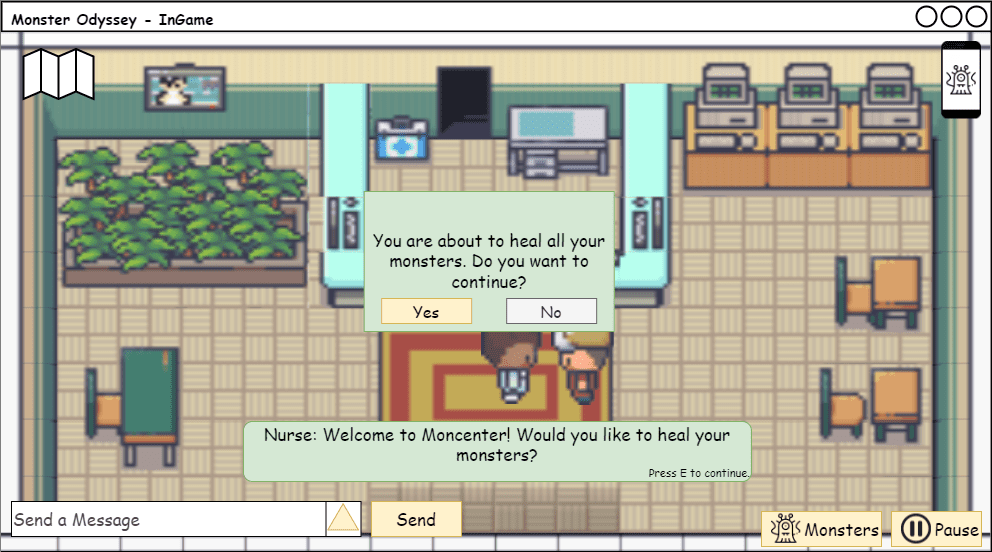
\includegraphics[width=\textwidth]{images/mockups/Heilung/PlayerInMoncenterHealingPopUp.png}
        \caption{Heilungsfenster beim Drücken der Interaktionstaste}
        \label{fig: Heilungsfenster}
    \end{subfigure}
    \caption{Mockup: Interaktion mit Krankenschwester in Moncenter}
    \label{fig: Interaktion mit Krankenschwester in Moncenter}
\end{figure}
Bei dem Pop-up aus der Abbildung~\ref{fig: Heilungsfenster} hat der Nutzer zwei Optionen: die Frage mit „Yes“ oder mit „No“ zu beantworten. Beim Drücken des 'Yes'-Knopfs werden die Monster des Nutzers geheilt und es öffnet sich ein neuer Dialog, in dem die Krankenschwester wie in Abbildung~\ref{fig: Monster geheilt} die Aktion bestätigt. 
Im Gegensatz dazu werden beim Drücken des 'No'-Knopfs die Monster nicht geheilt und die Krankenschwester weist den Nutzer wie in Abbildung~\ref{fig: Monster nicht geheilt} darauf hin, dass er jederzeit wieder in das 'Moncenter' kommen und seine Monster heilen kann.
\begin{figure}[H]
    \centering
    \begin{subfigure}[b]{0.4\textwidth}
        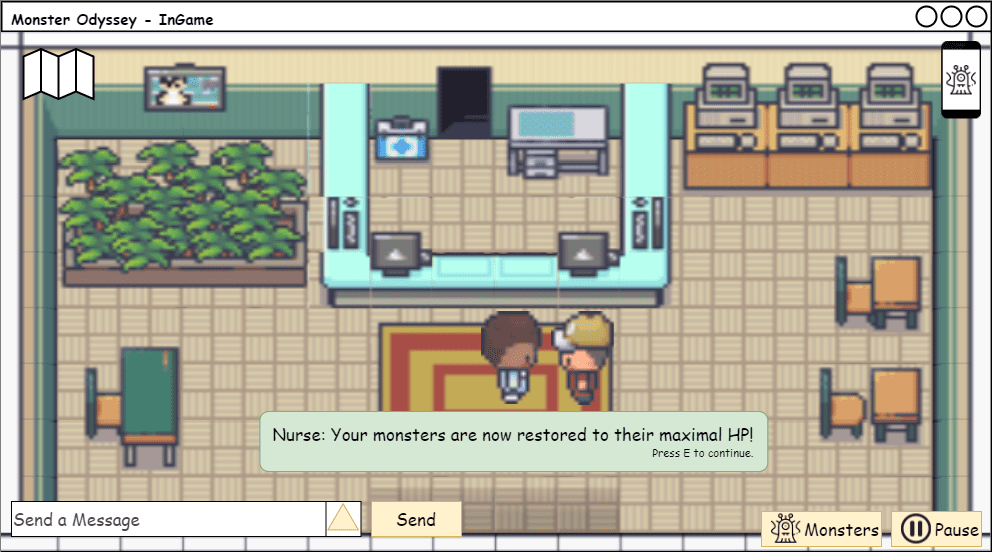
\includegraphics[width=\textwidth]{images/mockups/Heilung/PlayerInMoncenterHealingHealed.png}
        \caption{Monster geheilt}
        \label{fig: Monster geheilt}
    \end{subfigure}
    \hfill
    \begin{subfigure}[b]{0.4\textwidth}
        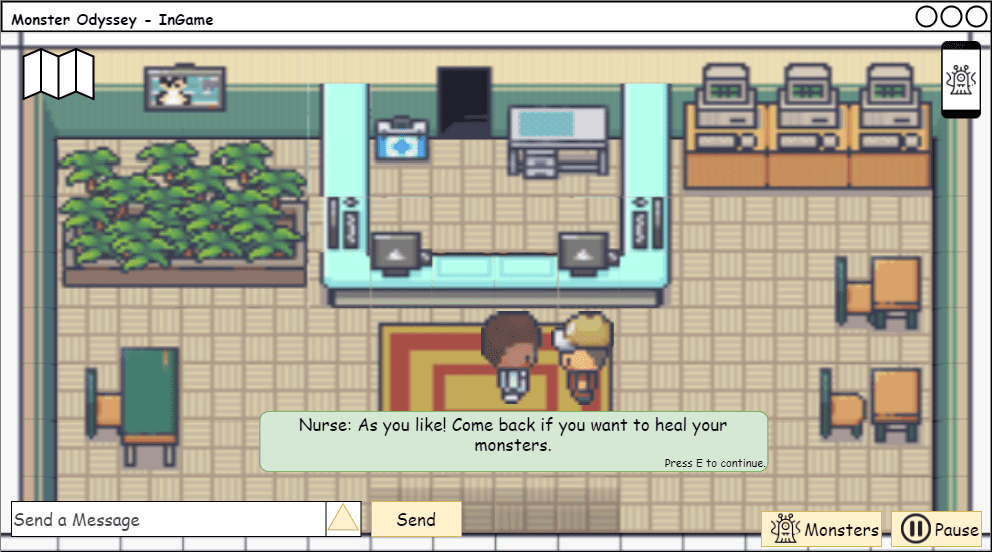
\includegraphics[width=\textwidth]{images/mockups/Heilung/PlayerInMoncenterHealingNotHealed.png}
        \caption{Monster nicht geheilt}
        \label{fig: Monster nicht geheilt}
    \end{subfigure}
    \caption{Mockup: Antwort der Krankenschwester}
    \label{fig: Antwort der Krankenschwester}
\end{figure}
\subsection{Vergleich zwischen Mockups und Implementierung}\label{subsec:vergleich-zwischen-mockups-und-implementierung-monster-heilen}
In der Abbildung~\ref{fig: Vergleich: Dialog zwischen Nutzer und Krankenschwester} ist anzumerken, dass sich die Position der Krankenschwester von dem Mockup unterscheidet. Demzufolge steht die Krankenschwester hinter der Theke in der Abbildung~\ref{fig: Implementierung: Dialog zwischen Nutzer und Krankenschwester}. Darüber hinaus ist ein Unterschied im Dialogtext vorhanden, der aus dem gleichen Grund wie in Abschnitt~\ref{subsec:vergleich-zwischen-mockups-und-implementierung-starter-monster} besteht.
\begin{figure}[H]
    \centering
    \begin{subfigure}[b]{0.4\textwidth}
        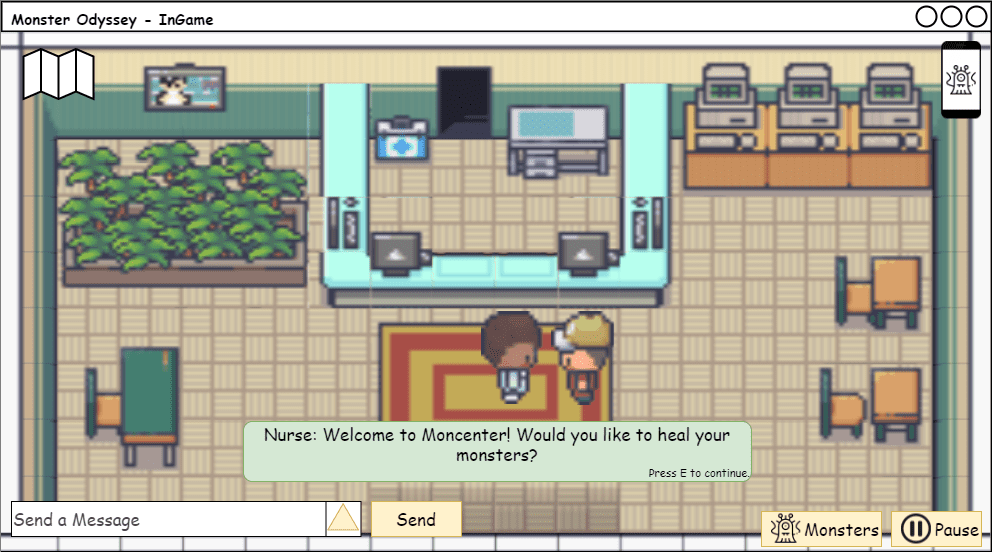
\includegraphics[width=\textwidth]{images/mockups/Heilung/PlayerInMoncenterHealingDialog.png}
        \caption{Mockup: Dialog Nutzer und Krankenschwester}
        \label{fig: Mockup: Dialog zwischen Nutzer und Krankenschwester}
    \end{subfigure}
    \hfill
    \begin{subfigure}[b]{0.4\textwidth}
        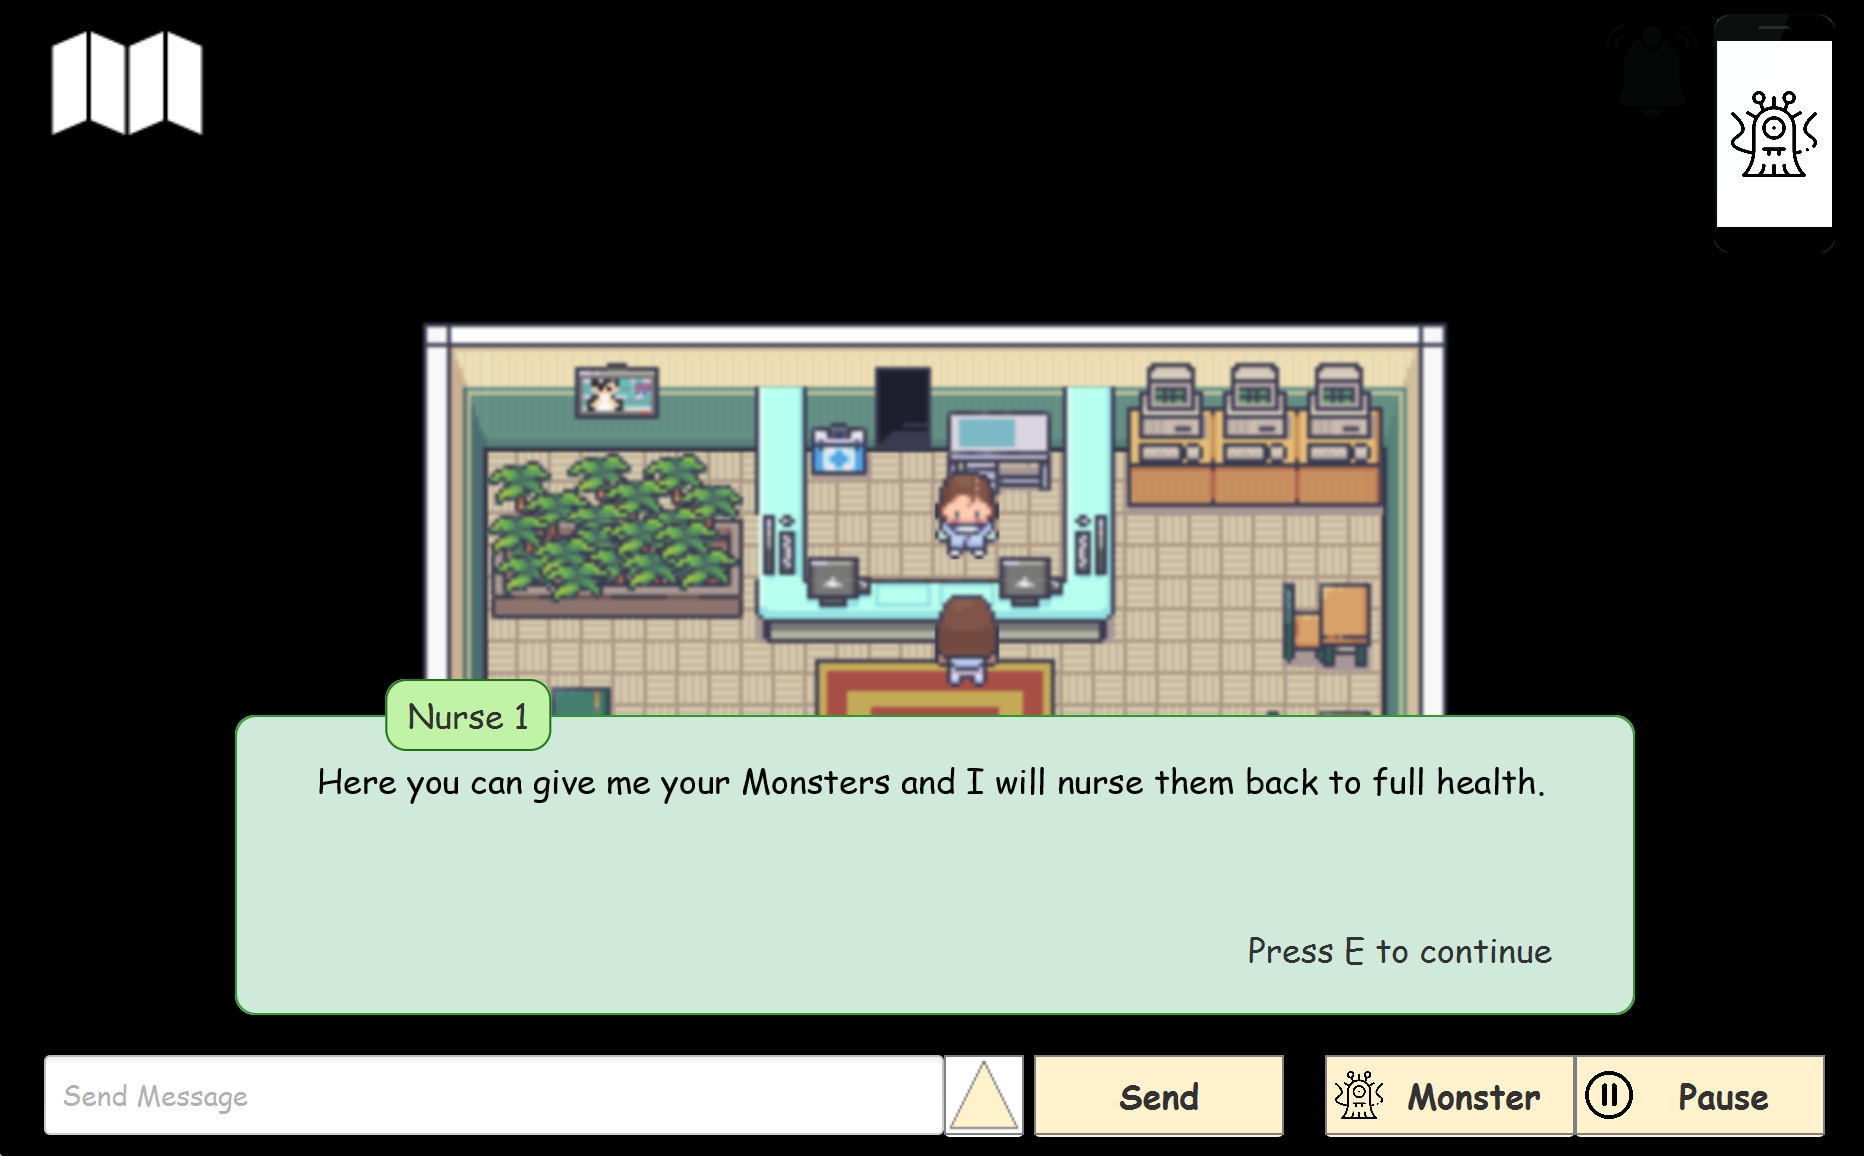
\includegraphics[width=\textwidth]{images/implementation/Heilung/DialogNurseImp.png}
        \caption{Implementierung: Dialog Nutzer und Krankenschwester}
        \label{fig: Implementierung: Dialog zwischen Nutzer und Krankenschwester}
    \end{subfigure}
    \caption{Vergleich: Dialog Nutzer und Krankenschwester}
    \label{fig: Vergleich: Dialog zwischen Nutzer und Krankenschwester}
\end{figure}
Ferner ist aus der Abbildung~\ref{fig: Vergleich: Heilungsfenster} zu erkennen, dass das Popup für das Heilungsfenster aus dem Mockup identisch mit der Implementierung ist, wobei auch hier ein Unschärfeeffekt für den Hintergrund ausgewählt worden ist. 
\begin{figure}[H]
    \centering
    \begin{subfigure}[b]{0.4\textwidth}
        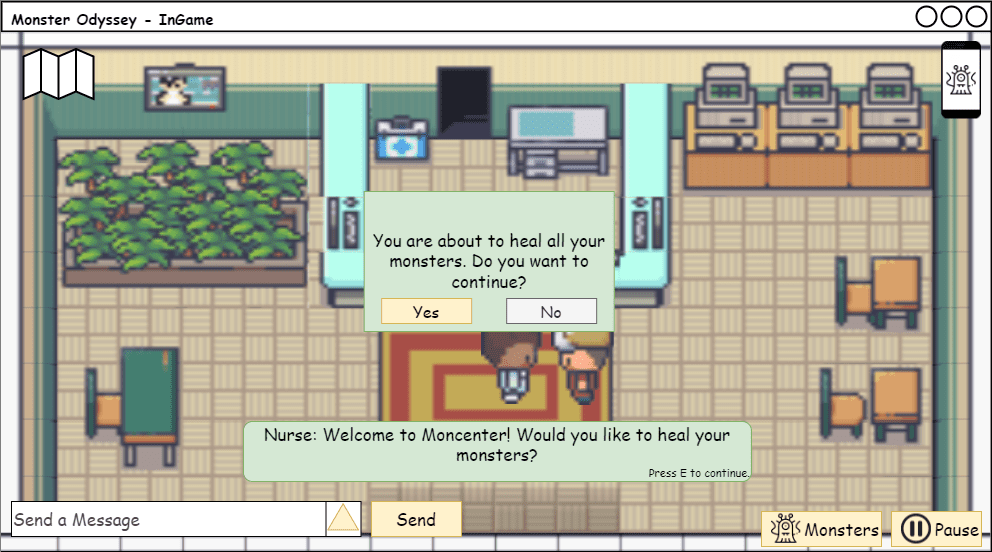
\includegraphics[width=\textwidth]{images/mockups/Heilung/PlayerInMoncenterHealingPopUp.png}
        \caption{Mockup: Heilungsfenster}
        \label{fig: Mockup: Heilungsfenster}
    \end{subfigure}
    \hfill
    \begin{subfigure}[b]{0.4\textwidth}
        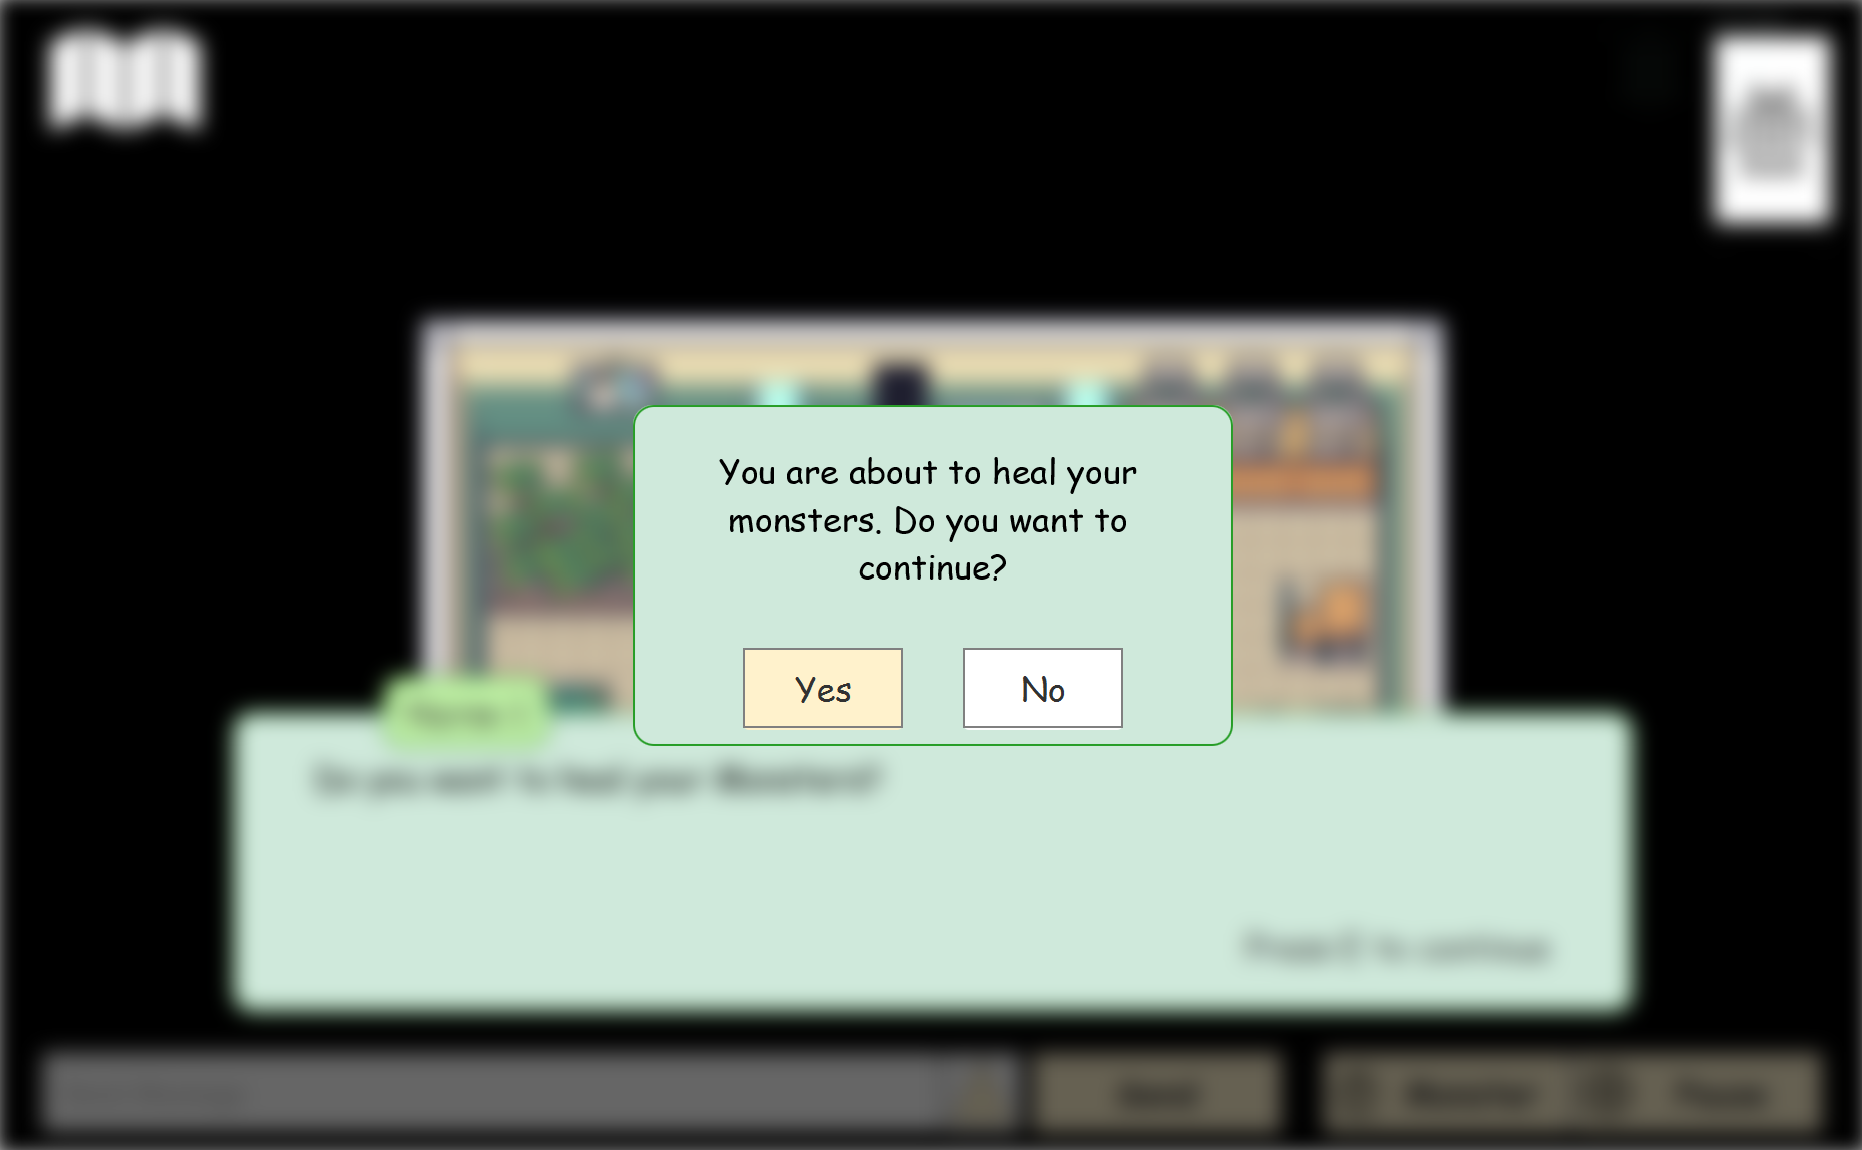
\includegraphics[width=\textwidth]{images/implementation/Heilung/PopupImplementation.png}
        \caption{Implementierung: Heilungsfenster}
        \label{fig: Implementierung: Heilungsfenster}
    \end{subfigure}
    \caption{Vergleich: Heilungsfenster}
    \label{fig: Vergleich: Heilungsfenster}
\end{figure}
\section{Kampfführung}\label{sec:kampf-führen}
Die Kampfführung ist die Hauptanforderung dieses Releases.
In einem Kampf kann der Nutzer seine Monster zum Einsatz bringen und interaktiv mit anderen Trainern spielen. Somit bildet diese Funktionalität die Kernfunktion des Spiels und stellt einen wichtigen Aspekt von\textit{ Monster Odyssey} dar.
\subsection{Mockups}\label{subsec:mockups-kampf-führen}
Die Kampfsituationen können variieren.
Der Nutzer kann beispielsweise in einem Eins-gegen-Eins-Szenario gegen einen anderen (NPC-)Trainer wie in Abbildung~\ref{fig: Eins-gegen-Eins Kampfsituation Trainer} oder gegen ein wildes Monster wie in Abbildung~\ref{fig: Eins-gegen-Eins Kampfsituation gegen wilden Monster} kämpfen. 
Darüber hinaus können zwei andere Kampfsituationen auftreten, sodass der Nutzer gegen zwei Trainer wie in Abbildung~\ref{fig: Eins-gegen-Zwei Kampfsituation} kämpfen soll und in der anderen Situation bekommt der Nutzer Unterstützung von einem anderen Trainer, wie in Abbildung~\ref{fig: Zwei-gegen-Zwei Kampfsituation} dargestellt ist.
Der Kampf ist in den unterschiedlichen Kampfsituationen ähnlich aufgebaut. Die Beschreibung des Aufbaus erfolgt im Folgenden anhand der Eins-gegen-Eins Kampfsituation aus der Abbildung~\ref{fig: Eins-gegen-Eins Kampfsituation}.
Die anderen Szenarien sind ähnlich angeordnet, sodass nur zusätzliche Trainer und Monster in Fällen der Eins-gegen-Zwei oder Zwei-gegen-Zwei wie in den Abbildungen~\ref{fig: Eins-gegen-Zwei Kampfsituation} und~\ref{fig: Zwei-gegen-Zwei Kampfsituation} hinzugefügt werden. Im Falle des Eins-gegen-Eins-Spiels gegen ein wildes Monster wie in der Abbildung~\ref{fig: Eins-gegen-Eins Kampfsituation gegen wilden Monster} wird die Trainerfigur entfernt.
Der Charakter des eigenen Trainers befindet sich auf der unteren Seite des Bildschirms.
Vor dem Trainer ist das aktuell ausgewählte Monster dargestellt. Damit kann der Nutzer die Fähigkeiten dieses Monsters für Angriffe auf die gegnerischen Monster anwenden.
Der Aufbau der gegnerischen Seite ist identisch mit der Seite des Nutzers, mit dem kleinen Unterschied, dass die Seiten gespiegelt sind.
Auf der gegnerischen Seite kann der Nutzer das jetzige Level, die aktuellen Lebenspunkte als Lebensbalken und den Namen des gegnerischen Monsters sehen. Auf der Seite des Nutzers sind dieselben Attribute vorhanden. Zusätzlich dazu kann der Nutzer die Erfahrungspunkte für den Levelaufstieg als Balken und Lebenspunkte als Zahl sehen.
Das Protokollieren der Kampfereignisse erfolgt in einem grünen Textfeld im unteren Bereich des Bildschirms. 
\begin{figure}[H]
    \centering
    \begin{subfigure}[b]{0.4\textwidth}
        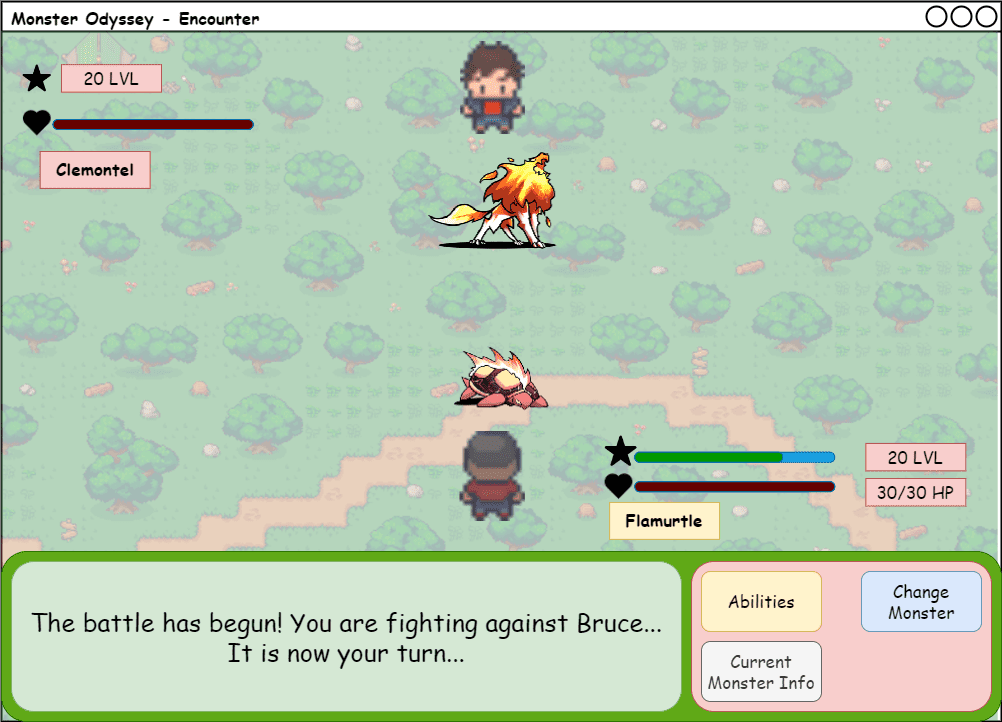
\includegraphics[width=\textwidth]{images/mockups/Encounter/Encounter1v1.png}
        \caption{Eins-gegen-Eins Kampfsituation Trainer}
        \label{fig: Eins-gegen-Eins Kampfsituation Trainer}
    \end{subfigure}
    \hfill
    \begin{subfigure}[b]{0.4\textwidth}
        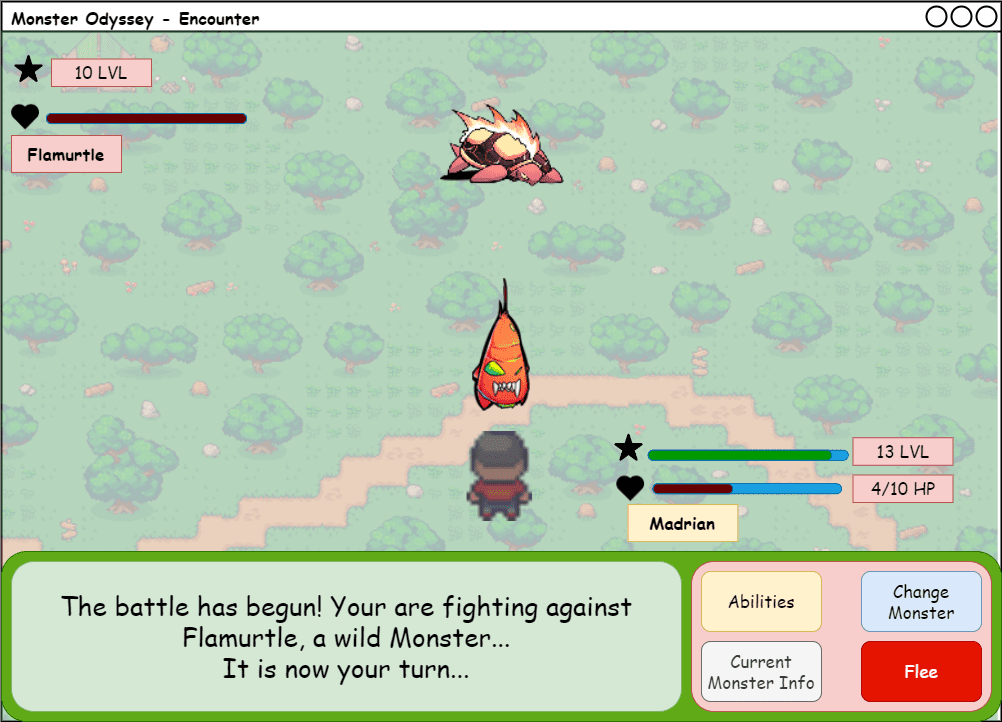
\includegraphics[width=\textwidth]{images/mockups/Encounter/EncounterWild.png}
        \caption{Eins-gegen-Eins Kampfsituation gegen wilden Monster}
        \label{fig: Eins-gegen-Eins Kampfsituation gegen wilden Monster}
    \end{subfigure}
    \caption{Mockup: Eins-gegen-Eins Kampfsituation}
    \label{fig: Eins-gegen-Eins Kampfsituation}
\end{figure}
\begin{figure}[H]
    \centering
    \begin{subfigure}[b]{0.4\textwidth}
        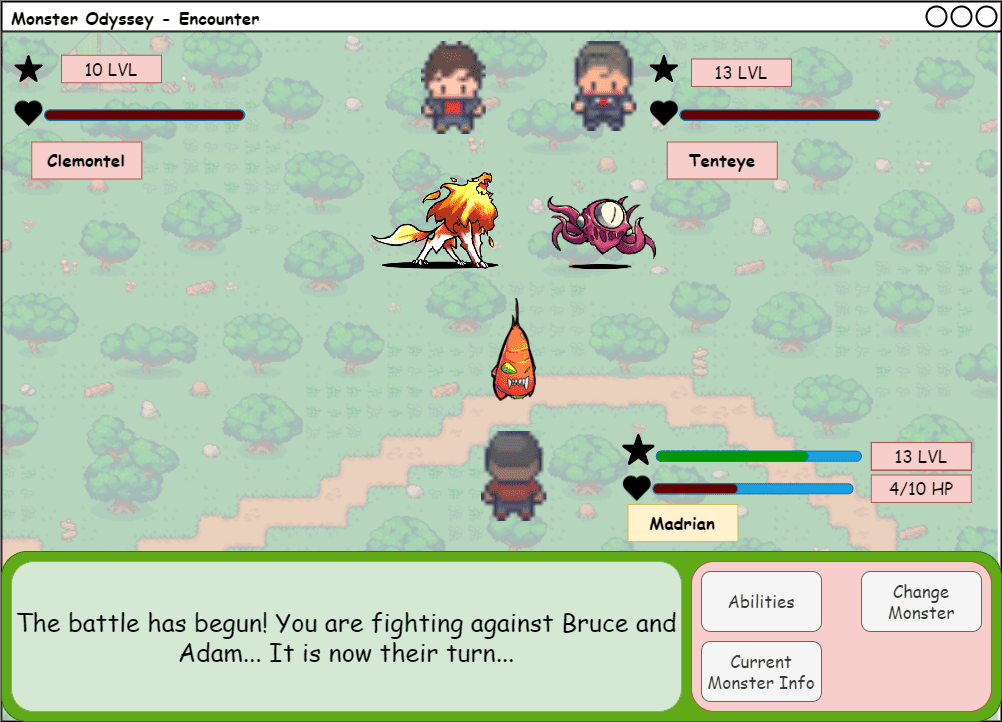
\includegraphics[width=\textwidth]{images/mockups/Encounter/Encounter1v2.png}
        \caption{Eins-gegen-Zwei Kampfsituation}
        \label{fig: Eins-gegen-Zwei Kampfsituation}
    \end{subfigure}
    \hfill
    \begin{subfigure}[b]{0.4\textwidth}
        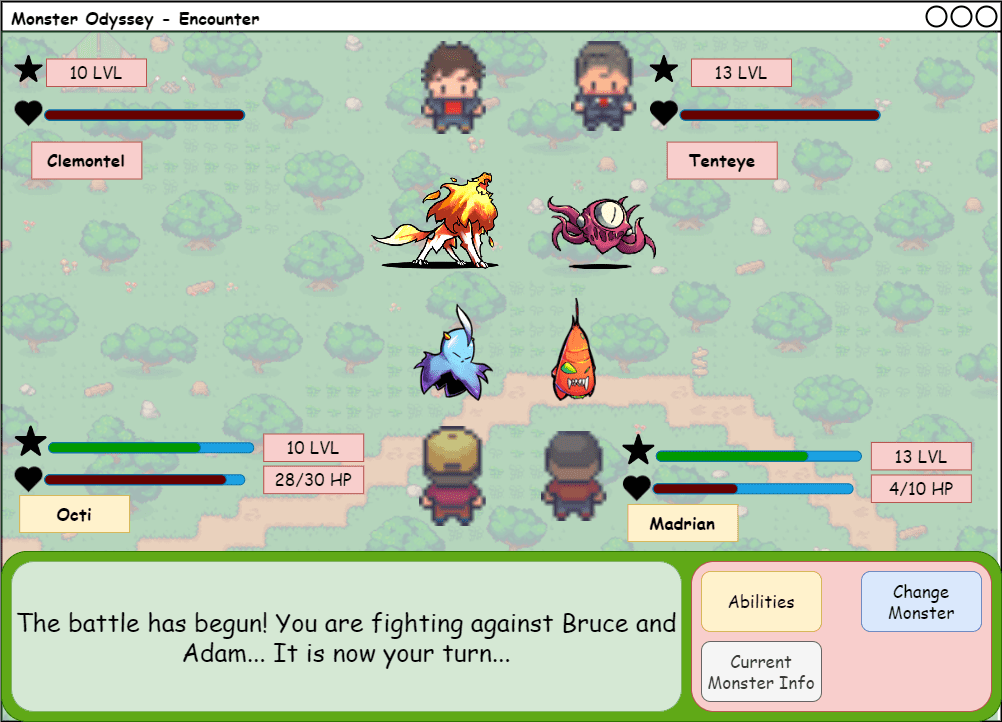
\includegraphics[width=\textwidth]{images/mockups/Encounter/Encounter2v2.png}
        \caption{Zwei-gegen-Zwei Kampfsituation}
        \label{fig: Zwei-gegen-Zwei Kampfsituation}
    \end{subfigure}
    \caption{Mockup: Eins-gegen-Zwei und Zwei-gegen-Zwei Kampfsituationen}
    \label{fig:Eins-gegen-Zwei und Zwei-gegen-Zwei Kampfsituationen}
\end{figure}
Neben dem Textfeld befinden sich mehrere Knöpfe, die für den Kampf essenziell sind. Die zwei Knöpfe 'Abilities' und 'Change Monster' sind unter Umständen deaktiviert und je nach Kontext werden sie wieder aktiviert und klickbar, wohingegen der Knopf 'Current Monster Info' jederzeit verfügbar ist.
Mit dem ersten Knopf 'Abilities' aus beispielsweise Abbildung~\ref{fig: Eins-gegen-Eins Kampfsituation Trainer} kann der Nutzer die Fähigkeiten des aktuellen Monsters sehen. 
Mit dem Drücken einer Fähigkeit wie in Abbildung~\ref{fig: Fähigkeiten des jetzigen Monsters} wird diese Fähigkeit für den Zug des Nutzers gesetzt und der Server entscheidet, wessen Fähigkeit von beiden Trainern ausgeführt und angewandt wird.
Wenn eine Fähigkeit angewandt wird, sieht der Nutzer eine Benachrichtigung wie in Abbildung~\ref{fig: Fähigkeit auf den gegnerischen Monster angewandt} in dem Textfeld, in der der Name der verwendeten Fähigkeit, der Name des angegriffenen Monsters und die Effektivität des Angriffs erwähnt sind.
Weiterhin werden alle Attribute, der vom Angriff betroffenen Monster, aktualisiert.
Der Nutzer muss mit der Nutzung der Fähigkeiten sparsam umgehen, da es für die jeweilige Fähigkeit eine begrenzte Anzahl an Nutzungen, wie in der Abbildung~\ref{fig: Fähigkeiten des jetzigen Monsters} zu sehen ist, gibt.
Die Anzahl an übrigen Nutzungen sieht der Nutzer unter dem Namen der Fähigkeit in dem Knopf.
Darüber hinaus kann der Nutzer zu der ursprünglichen Ansicht aus der Abbildung~\ref{fig: Eins-gegen-Eins Kampfsituation Trainer} zurückkehren, wenn er den Pfeilknopf drückt.
\begin{figure}[H]
    \center
    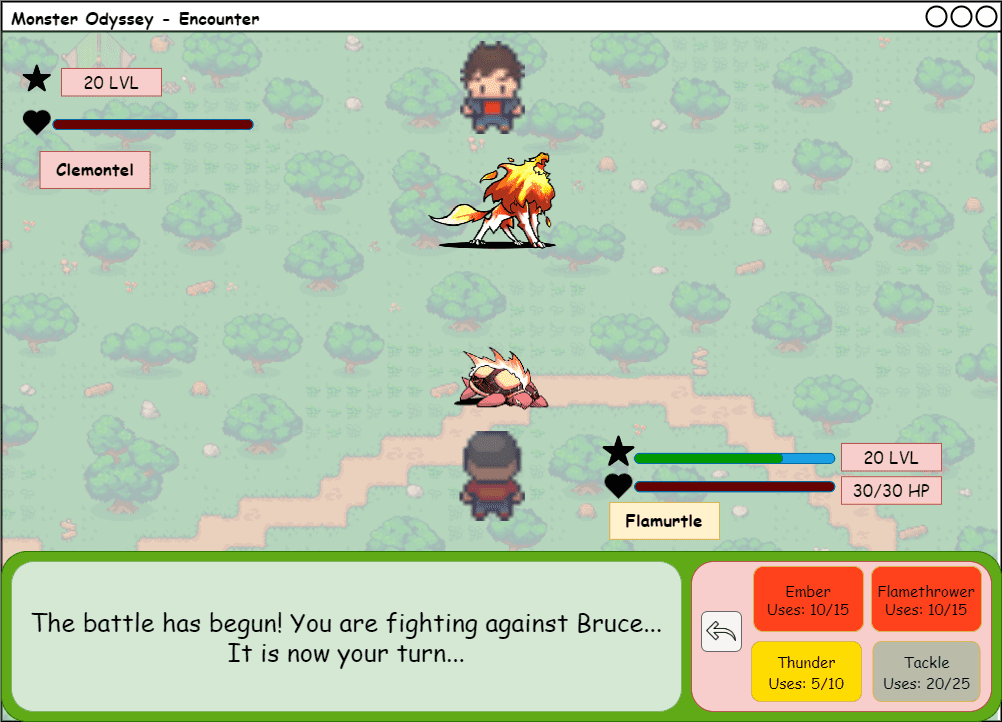
\includegraphics[scale=\scale]{images/mockups/Encounter/Encounter1v1Abilities.png}
    \caption{Mockup: Fähigkeiten des jetzigen Monsters}
    \label{fig: Fähigkeiten des jetzigen Monsters}
\end{figure}
\begin{figure}[H]
    \center
    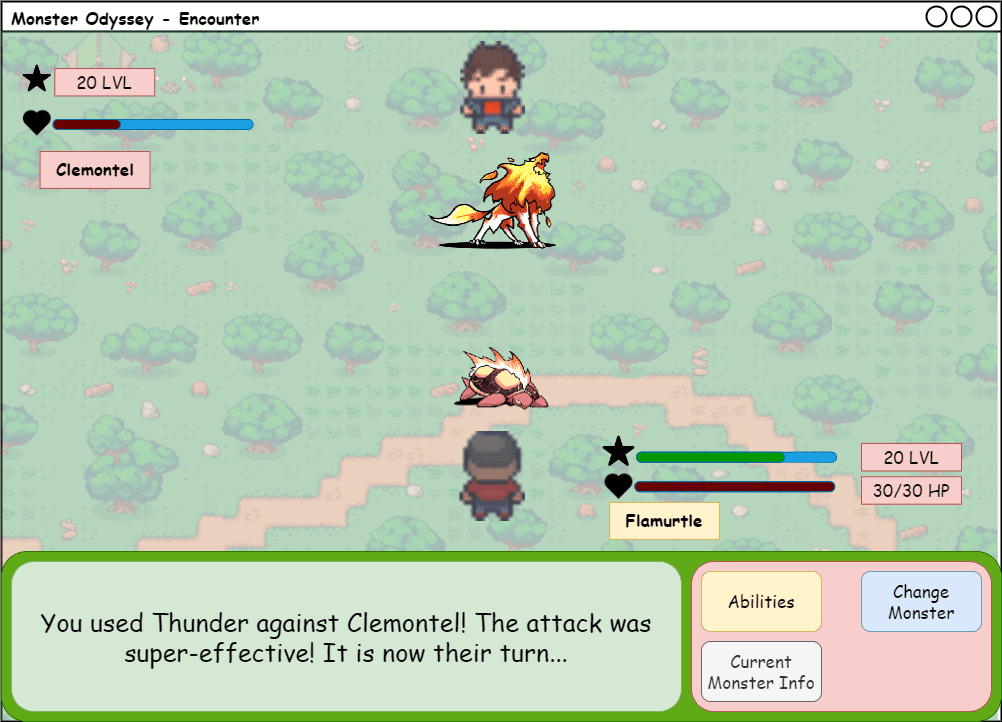
\includegraphics[scale=\scale]{images/mockups/Encounter/Encounter1v1AbilitiesUsed.png}
    \caption{Mockup: Fähigkeit auf das gegnerische Monster angewandt}
    \label{fig: Fähigkeit auf den gegnerischen Monster angewandt}
\end{figure}
Der Nutzer besiegt das gegnerische Monster, wenn seine Lebenspunkte auf null gesetzt sind.
Die Benachrichtigung in dem Textfeld wird entsprechend der Abbildung~\ref{fig: Gegnerischen Monster besiegt} angezeigt. 
Dabei erhält das jetzige Monster Erfahrungspunkte.
Sobald diese ausreichend für einen Levelaufstieg sind, bekommt der Monster neue persistente Attribute (Level, Schaden, max. Lebenspunkte, Geschwindigkeit und Verteidigung) und erlernt eine neue Fähigkeit, die in einem Fenster, wie in Abbildung~\ref{fig: Levelup mit neuen Werten und neuer Fähigkeit} zu sehen ist, dargestellt sind. 
Für die erlernte Fähigkeit werden der Name, eine kurze Beschreibung, die Stärke, die Präzision, die Anzahl der maximalen Nutzungen und der Typ der Fähigkeit angezeigt. 
Diese Fähigkeit wird nur dann erlernt, wenn das Monster weniger als vier Fähigkeiten besitzt.
Falls das Monster bereits vier Fähigkeiten aufweist, erscheint das Fenster ohne die erlernte Fähigkeit wie in Abbildung~\ref{fig: Levelup mit neuen Werten} aufgezeigt ist.

Sofern der Gegner keine anderen Monster mit Lebenspunkten \textgreater  0 hat, verliert der er den Kampf während der Nutzer den Kampf gewinnt. 
Es erscheint ein Popup, in welchem der Nutzer über den Gewinn, wie in der Abbildung~\ref{fig: Encounter gewonnen Ankündigung} gezeigt ist und über das Verlassen der Kampfszene beachrichtigt wird.
Die Kampfszene wird erst verlassen und zum Spielbildschirm gewechselt, sobald der Nutzer auf den 'OK'-Knopf aus der Abbildung~\ref{fig: Encounter gewonnen Ankündigung} gedrückt hat.
Falls der Gegner das aktuelle Monster des Nutzers, wie in Abbildung~\ref{fig: Jetziger Monster besiegt} dargestellt ist, besiegt und der Nutzer kein anderes Monster mit Lebenspunkten \textgreater  0 besitzt, erscheint ein Popup wie in Abbildung~\ref{fig: Encounter verloren Ankündigung} mit der gleichen Funktionalität wie das Popup aus Abbildung~\ref{fig: Encounter gewonnen Ankündigung}.
\begin{figure}[H]
    \center
    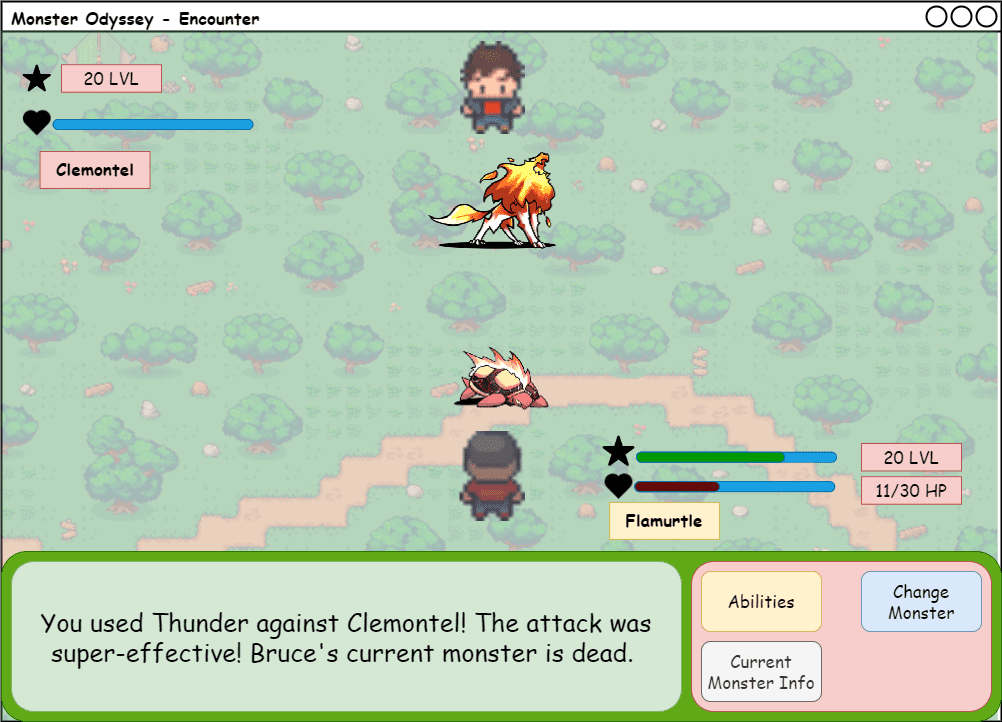
\includegraphics[scale=\scale]{images/mockups/Encounter/Encounter1v1AbilitiesUsedWon.png}
    \caption{Mockup: Gegnerischer Monster besiegt}
    \label{fig: Gegnerischen Monster besiegt}
\end{figure}
\begin{figure}[H]
    \center
    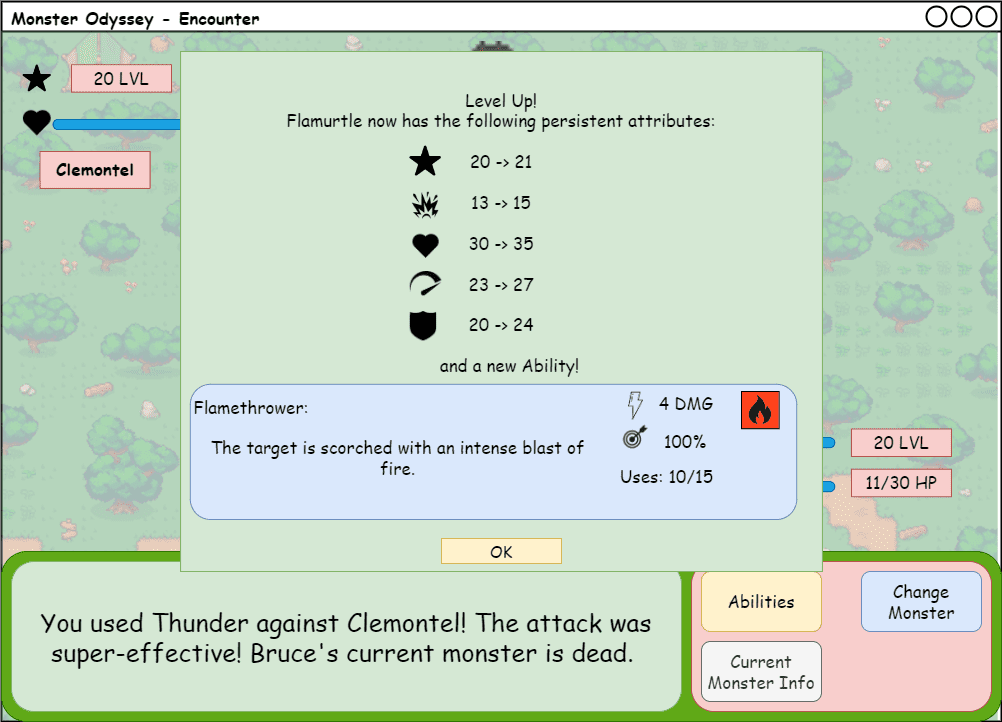
\includegraphics[scale=\scale]{images/mockups/Encounter/Encounter1v1AbilitiesUsedWonLevelUp.png}
    \caption{Mockup: Levelup mit neuen Werten und neuer Fähigkeit}
    \label{fig: Levelup mit neuen Werten und neuer Fähigkeit}
\end{figure}
\begin{figure}[H]
    \center
    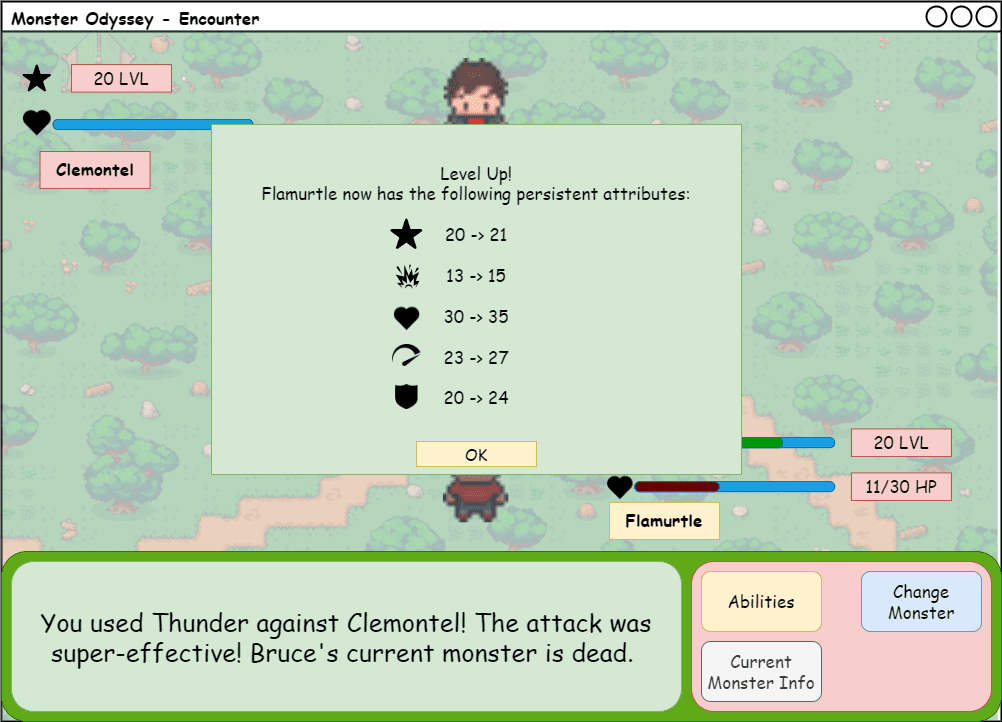
\includegraphics[scale=\scale]{images/mockups/Encounter/Encounter1v1AbilitiesUsedWonLevelUpNoAbility.png}
    \caption{Mockup: Levelup mit neuen Werten}
    \label{fig: Levelup mit neuen Werten}
\end{figure}
\begin{figure}[H]
    \center
    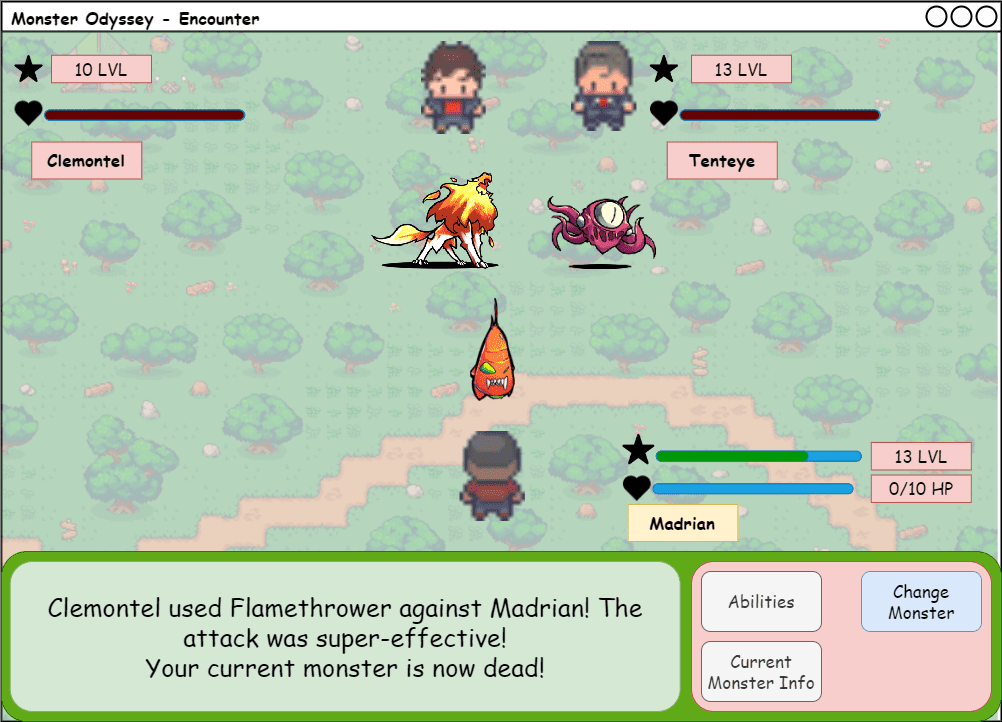
\includegraphics[scale=\scale]{images/mockups/Encounter/Encounter1v2OpponentAttackedAndLost.png}
    \caption{Mockup: Jetziger Monster besiegt}
    \label{fig: Jetziger Monster besiegt}
\end{figure}
\begin{figure}[H]
    \centering
    \begin{subfigure}[b]{0.4\textwidth}
        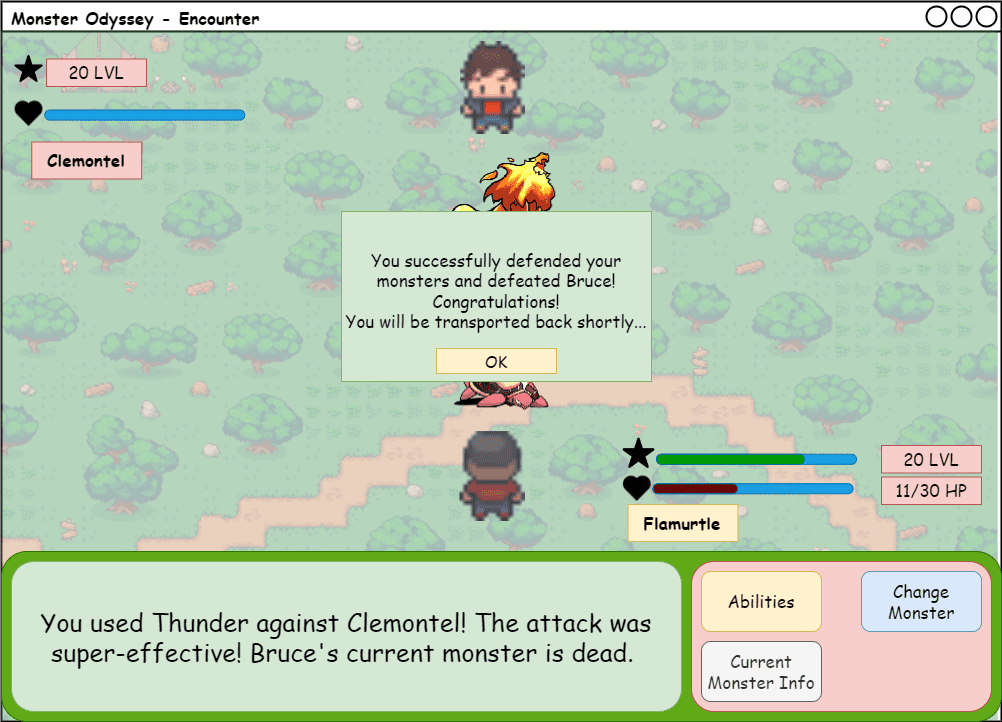
\includegraphics[width=\textwidth]{images/mockups/Encounter/Encounter1v1AbilitiesUsedWonGoBack.png}
        \caption{Kampf gewonnen}
        \label{fig: Encounter gewonnen Ankündigung}
    \end{subfigure}
    \hfill
    \begin{subfigure}[b]{0.4\textwidth}
        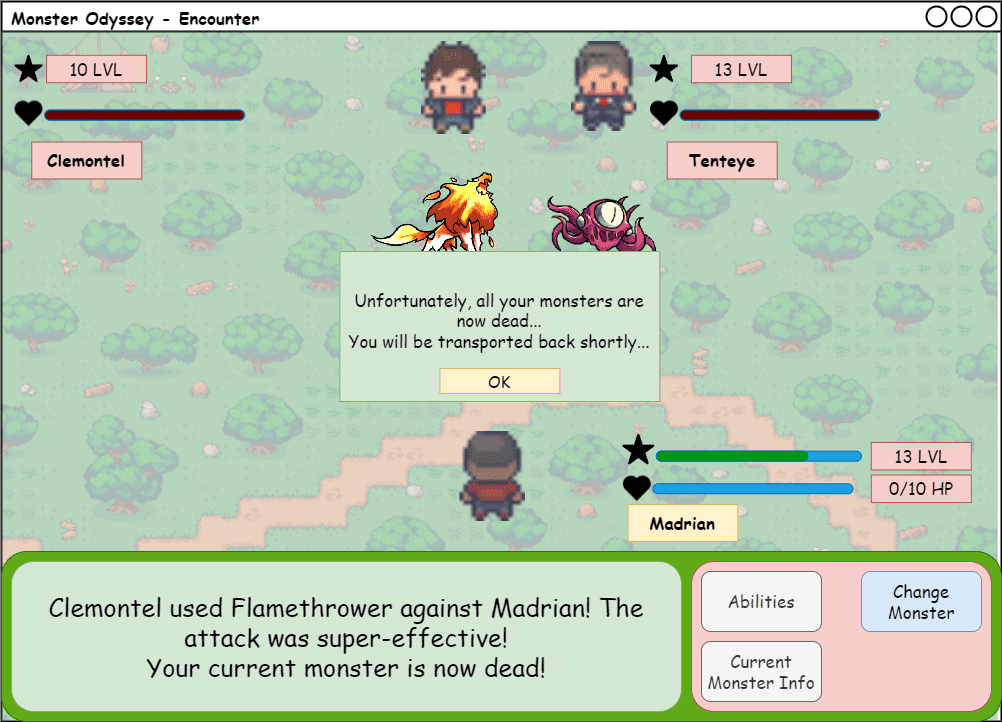
\includegraphics[width=\textwidth]{images/mockups/Encounter/Encounter1v2OpponentAttackedAndLostPopup.png}
        \caption{Kampf verloren}
        \label{fig: Encounter verloren Ankündigung}
    \end{subfigure}
    \caption{Mockup: Kampf beendet}
    \label{fig: Encounter beendet}
\end{figure}
Der Nutzer hat außerdem die Gelegenheit, Informationen über das aktuelle Monster aufzurufen. Dabei werden verschiedene Attribute für das Monster dargestellt, die für den Kampf eine hohe Relevanz aufweisen. Das Informationsfenster erscheint, wenn der Nutzer den Knopf 'Current Monster Info' aus Abbildung~\ref{fig: Informationen über den jetzigen Monster} drückt. In dem Fenster aus Abbildung~\ref{fig: Informationen über den jetzigen Monster} kann der Nutzer das Bild, die persistenten und aktuellen Attribute als Balken und Zahl, den Typen und die Fähigkeiten des Monsters sehen. Für die jeweilige Fähigkeit ist eine Übersicht, wie in Abbildung~\ref{fig: Levelup mit neuen Werten und neuer Fähigkeit} gezeigt ist, für die erlernte Fähigkeit vorhanden.  
\begin{figure}[H]
    \center
    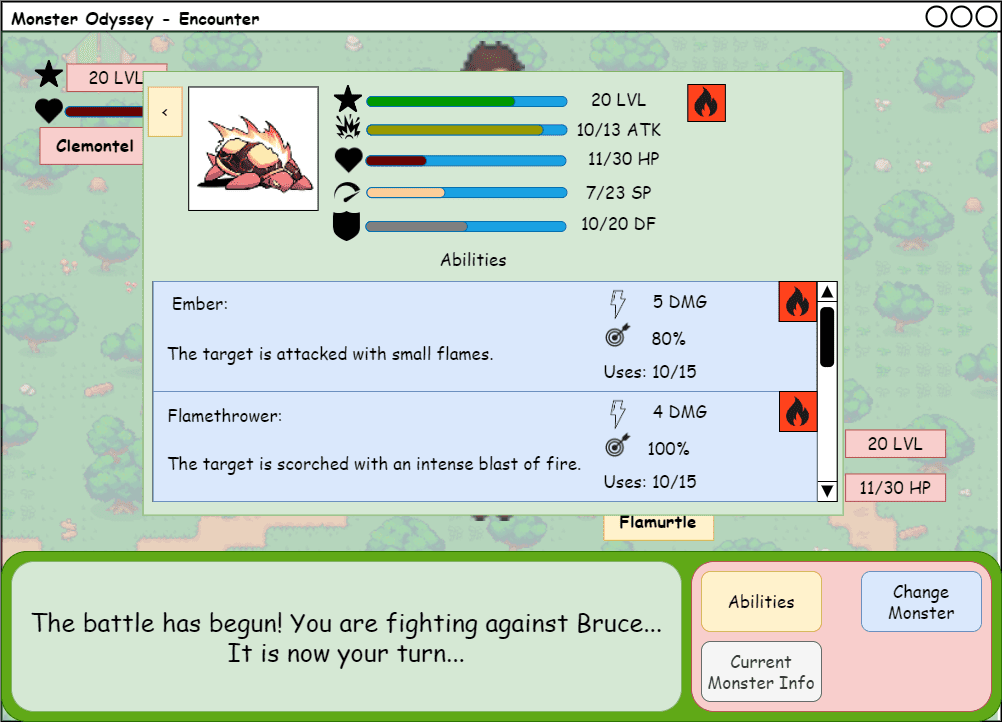
\includegraphics[scale=\scale]{images/mockups/Encounter/Encounter1v1Info.png}
    \caption{Mockup: Informationen über den jetzigen Monster}
    \label{fig: Informationen über den jetzigen Monster}
\end{figure}
Befindet sich der Nutzer in einer Eins-gegen-Zwei oder Zwei-gegen-Zwei Kampfsituation und der Nutzer möchte eine Fähigkeit anwenden, dann muss der Nutzer das Ziel auswählen, mit welchem gegnerische Monster angegriffen werden sollen. 
Dem Nutzer wird wie in Abbildung~\ref{fig: Ziel auswählen} ein Hinweis gegeben. Der Nutzer wird aufgefordert auf das gewünschte gegnerische Monster zu klicken, um das Ziel auszuwählen. 
\begin{figure}[H]
    \center
    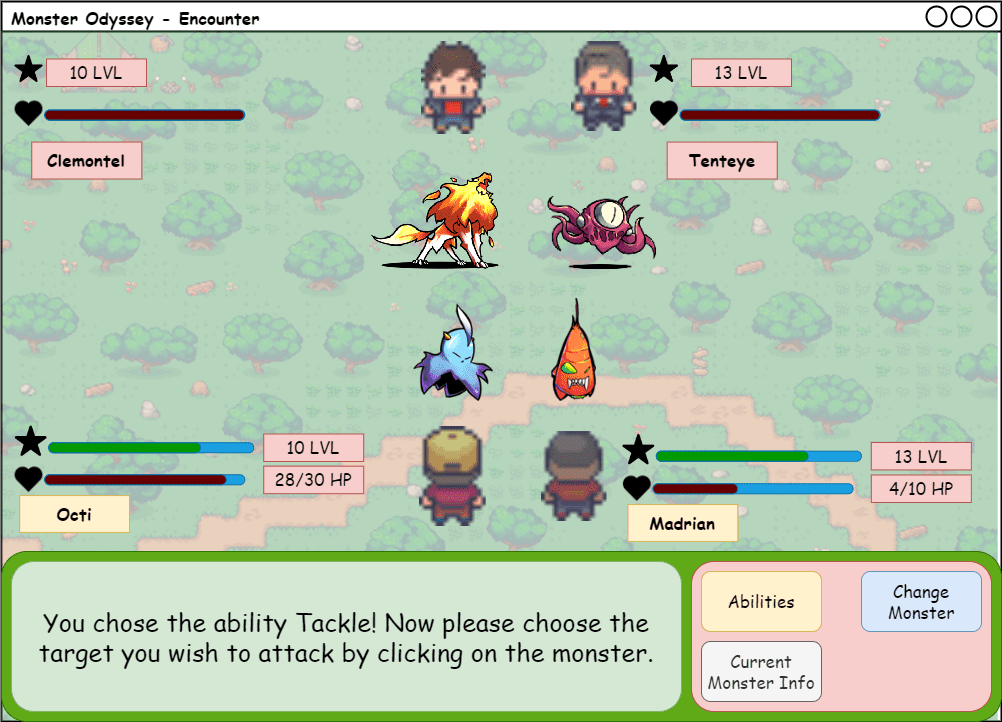
\includegraphics[scale=\scale]{images/mockups/Encounter/Encounter2v2ChooseTarget.png}
    \caption{Mockup: Ziel auswählen}
    \label{fig: Ziel auswählen}
\end{figure}
Es können Kampfsituationen auftreten, in denen das jetzige Monster schwächer als das gegnerische Monster wird. 
In diesem Fall hat der Nutzer die Möglichkeit das jetzige Monster gegen ein stärkeres Monster aus seinem Team auszuwechseln, indem der Nutzer auf den 'Change Monster'-Knopf aus Abbildung~\ref{fig: Monster wechseln Popup} drückt. 
Damit öffnet sich ein Fenster wie in Abbildung~\ref{fig: Monster wechseln Popup}, in welchem die verfügbaren Monster aus dem Team des Nutzers aufgelistet sind. Für jedes Monster auf der Liste gibt es zwei Knöpfe: einen Knopf für die Monsterinformationen und einen Knopf zum Wechseln des aktiven Monsters. 
Nach der Auswahl eines neuen aktiven Monster erscheint dieses Monster wie in Abbildung~\ref{fig: Monster ausgewechselt} vor der Trainerfigur des Nutzers und alle Attribute werden entsprechend aktualisiert.
Außerdem wird der Nutzer in dem Protokoll auf das Ereignis hingewiesen. 
\begin{figure}[H]
    \centering
    \begin{subfigure}[b]{0.4\textwidth}
        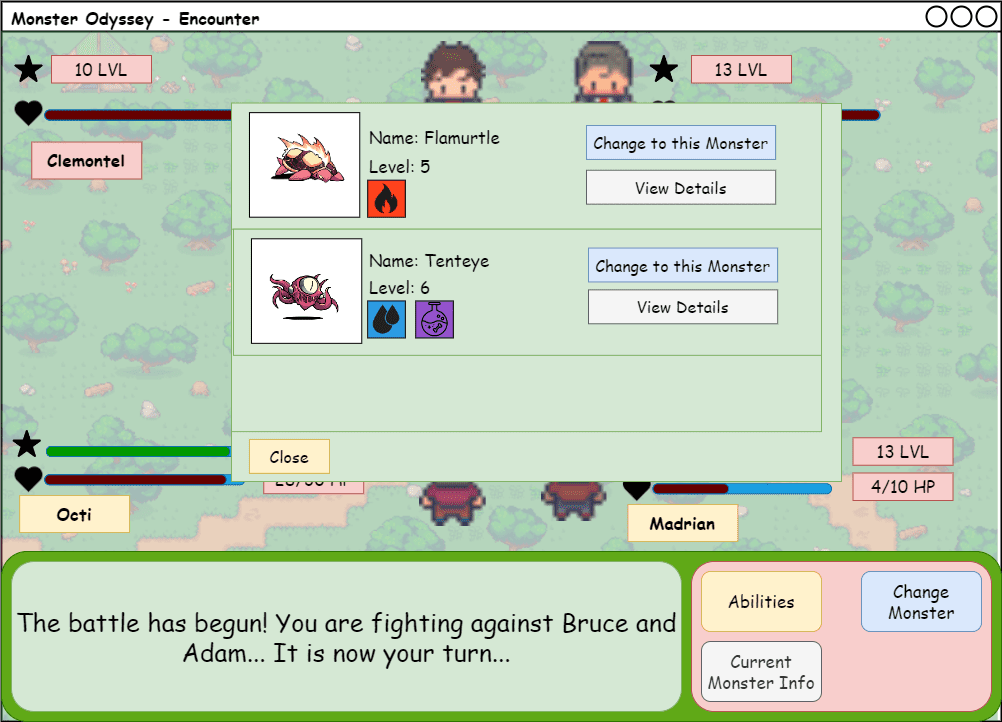
\includegraphics[width=\textwidth]{images/mockups/Encounter/Encounter2v2ChangeMonsterPopup.png}
        \caption{Monster auswechseln Popup}
        \label{fig: Monster wechseln Popup}
    \end{subfigure}
    \hfill
    \begin{subfigure}[b]{0.4\textwidth}
        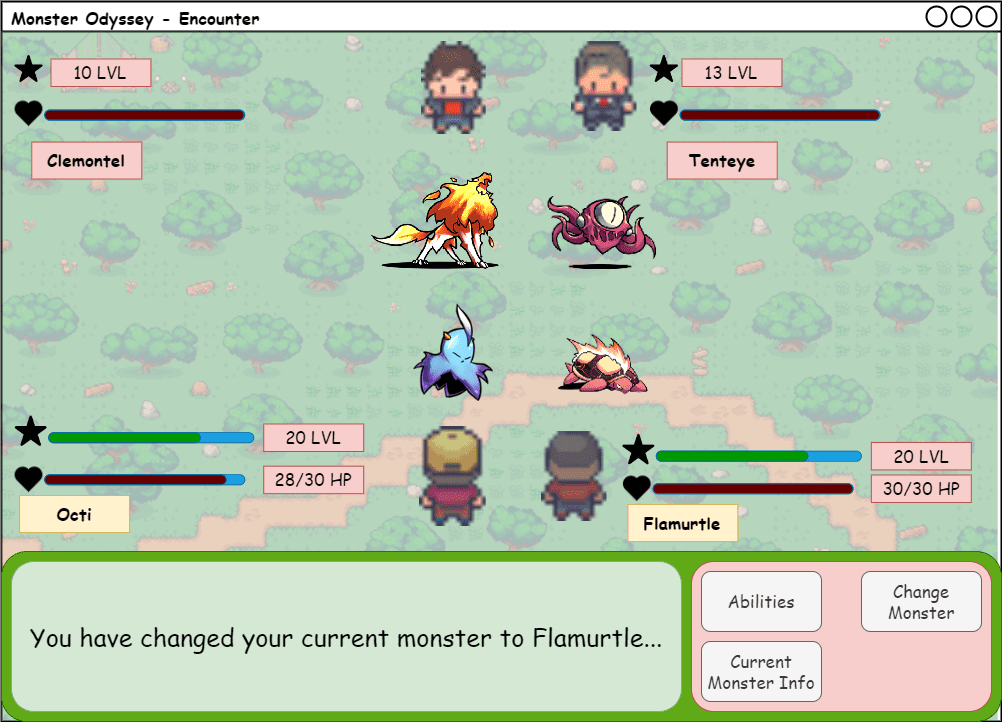
\includegraphics[width=\textwidth]{images/mockups/Encounter/Encounter2v2ChangeMonster.png}
        \caption{Monster ausgewechselt}
        \label{fig: Monster ausgewechselt}
    \end{subfigure}
    \caption{Mockup: Monster auswechseln}
    \label{fig: Monster auswechseln}
\end{figure}
Begegnet der Nutzer einem wilden Monster in hohem Gras und möchte gegen dieses Monster nicht kämpfen, dann kann der Nutzer aus dem Kampf fliehen, was bei den restlichen Kampfsituationen nicht möglich ist.
Der Nutzer kann aus dem Kampf beim Drücken auf den 'Flee'-Knopf aus der Abbildung~\ref{fig: Von wildem Monster fliehen Popup} fliehen. Somit wird ein Popup, wie in Abbildung~\ref{fig: Von wildem Monster fliehen Popup} angezeigt, in dem die Bestätigung des Nutzers für die Aktion benötigt wird.
Beim Drücken auf 'No' wird der Kampf fortgesetzt und beim Drücken auf 'Yes' wird das Fliehen bestätigt.
Anschließend wird der Nutzer in dem Ereignisprotokoll wie in Abbildung~\ref{fig: Von wildem Monster geflohen} darauf hingewiesen, dass der Nutzer aus der Kampfszene geflohen ist und die Szene in Kürze zum Spielbildschirm gewechselt wird. Das Wechseln der Szene erfolgt dann wenige Sekunden nach der Bekanntgabe. 
\begin{figure}[H]
    \centering
    \begin{subfigure}[b]{0.4\textwidth}
        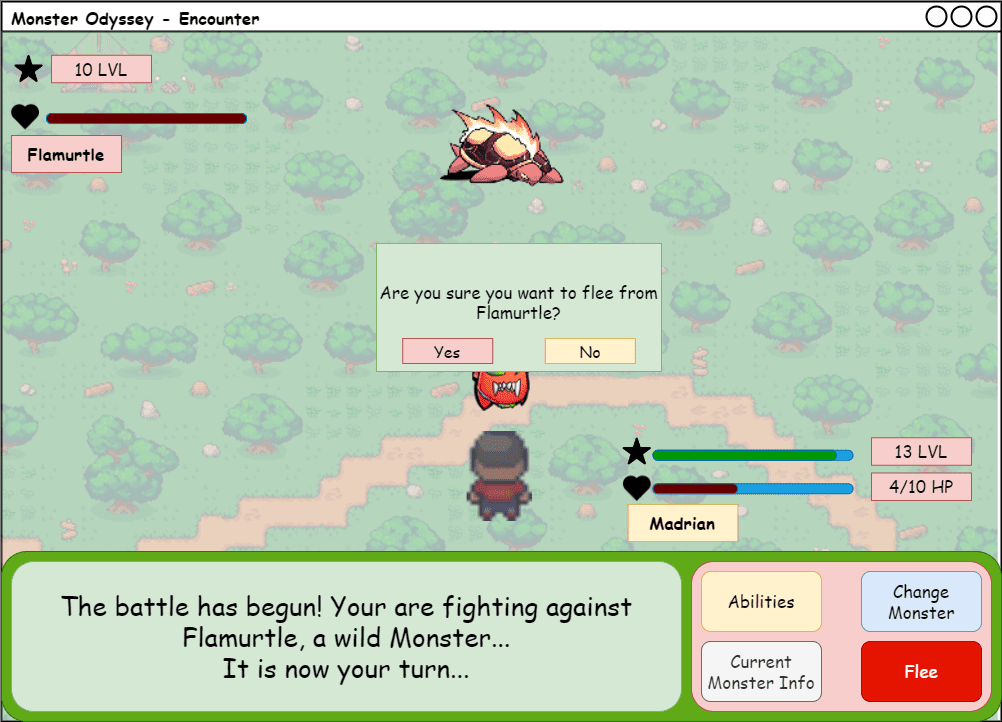
\includegraphics[width=\textwidth]{images/mockups/Encounter/EncounterWildFleePopUp.png}
        \caption{Popup beim Fliehen}
        \label{fig: Von wildem Monster fliehen Popup}
    \end{subfigure}
    \hfill
    \begin{subfigure}[b]{0.4\textwidth}
        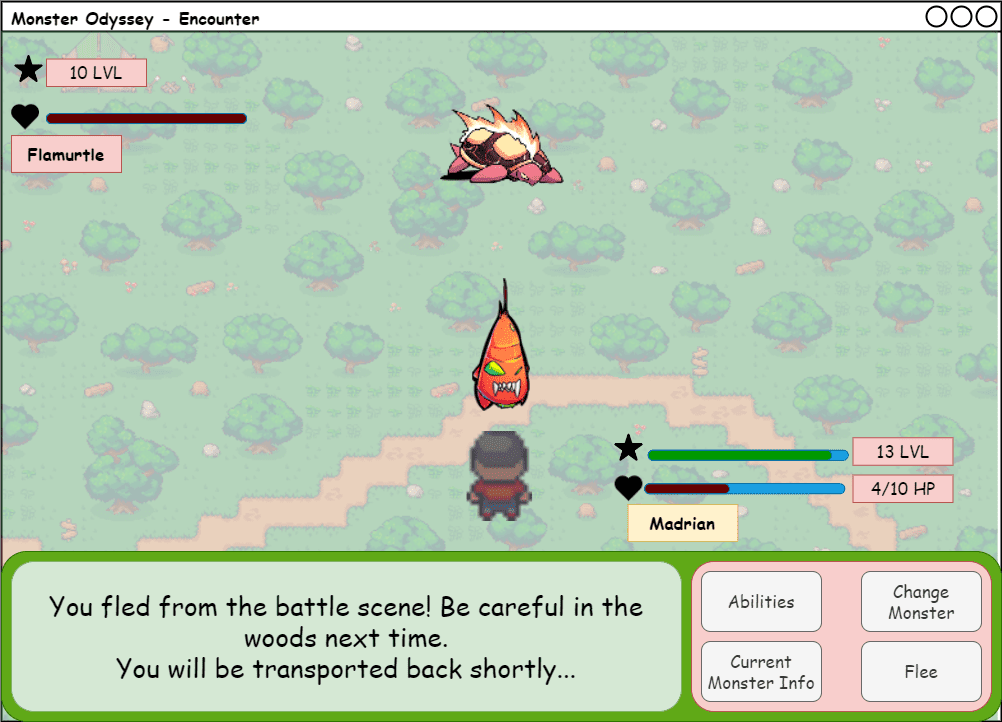
\includegraphics[width=\textwidth]{images/mockups/Encounter/EncounterWildFleed.png}
        \caption{Von wildem Monster geflohen}
        \label{fig: Von wildem Monster geflohen}
    \end{subfigure}
    \caption{Mockup: Fliehen von einem wilden Monster}
    \label{fig: Fliehen von einem wilden Monster}
\end{figure}

\subsection{Vergleich zwischen Mockups und Implementierung}\label{subsec:vergleich-zwischen-mockups-und-implementierung-kampf-führen}
Es bestehen viele Unterschiede zwischen den Mockups und der Implementierung, die auf der Ästhetik beziehungsweise der besseren Handhabung basieren. Im Folgenden werden die Unterschiede anhand der Szenarien Eins-gegen-Eins gegen einen Trainer und ein wildes Monster verdeutlicht. In der Abbildung~\ref{fig: Vergleich: Eins-gegen-Eins Kampfsituation Trainer} sind verschiedene Unterschiede anzumerken. Die Symbole für die Attribute 'Level' und 'Lebenspunkte' sind für die Übersichtlichkeit mit einer entsprechenden Farbe gekennzeichnet.
Der Namensbehälter von den Monstern ist etwas größer gestaltet, da es Monster mit längeren Namen gibt, die entsprechend mehr Platz benötigen.
Außerdem ist die Position des gegnerischen Trainers nach rechts verschoben. Der Grund der Verschiebung beruht auf der dynamischen Anzahl der gegnerischen Trainer, damit das Betreten eines neuen Trainers in den Kampf erleichtert wird.
Darüber hinaus sind die Balken größer und mit weißem Hintergrund ausgestattet. Das genaue Design aus den Mockups konnte wegen des Schwierigkeitsgrads nicht erzielt werden, wobei der weiße Hintergrund für eine klare Trennung zwischen dem maximalen Wert und dem tatsächlichem Wert sorgt.
Zudem ist die Darstellung der Lebenspunkte der Monster, die von dem Server vorgegebenen sind, mit einer Kommazahl anstatt einer ganzen Zahl ausgestattet.
In dem Ereignisprotokoll ist der letzte Satz weggelassen worden, da die Züge nicht nacheinander stattfinden, sondern beide Trainer ihren Zug gleichzeitig tätigen. Dabei ist der Text für das Ereignisprotokoll in fettgedruckter Schreibweise formuliert, was für den Nutzer eine bessere Lesbarkeit gewährleistet.
\begin{figure}[H]
    \centering
    \begin{subfigure}[b]{0.4\textwidth}
        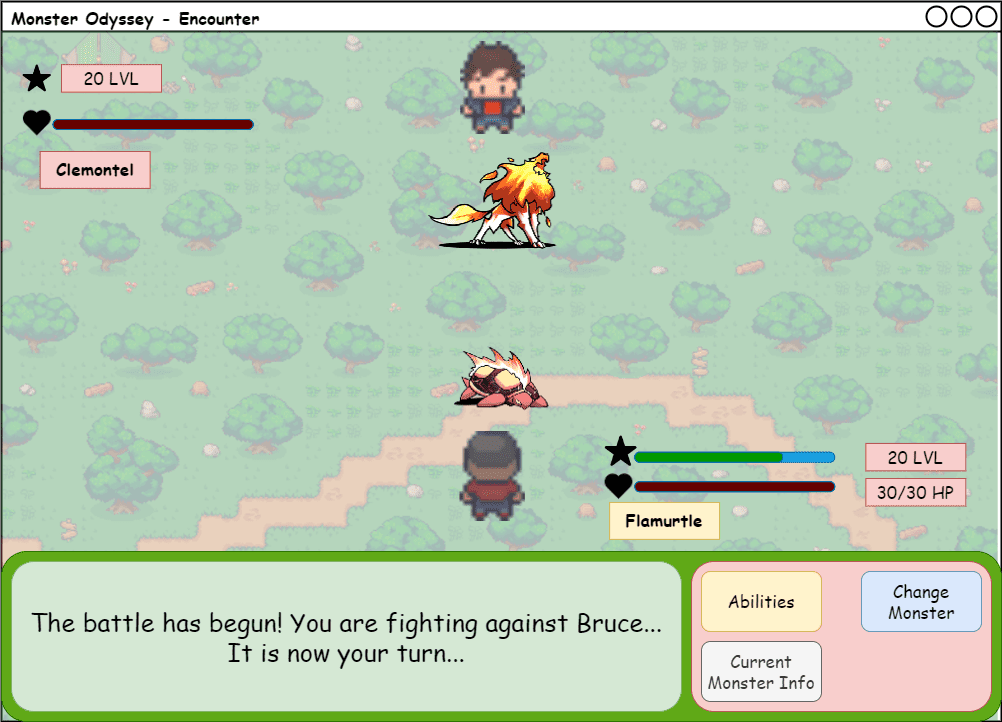
\includegraphics[width=\textwidth]{images/mockups/Encounter/Encounter1v1.png}
        \caption{Mockup:\phantom{EinsEins} Eins-gegen-Eins Kampfsituation Trainer}
        \label{fig: Mockup: Eins-gegen-Eins Kampfsituation Trainer}
    \end{subfigure}
    \hfill
    \begin{subfigure}[b]{0.4\textwidth}
        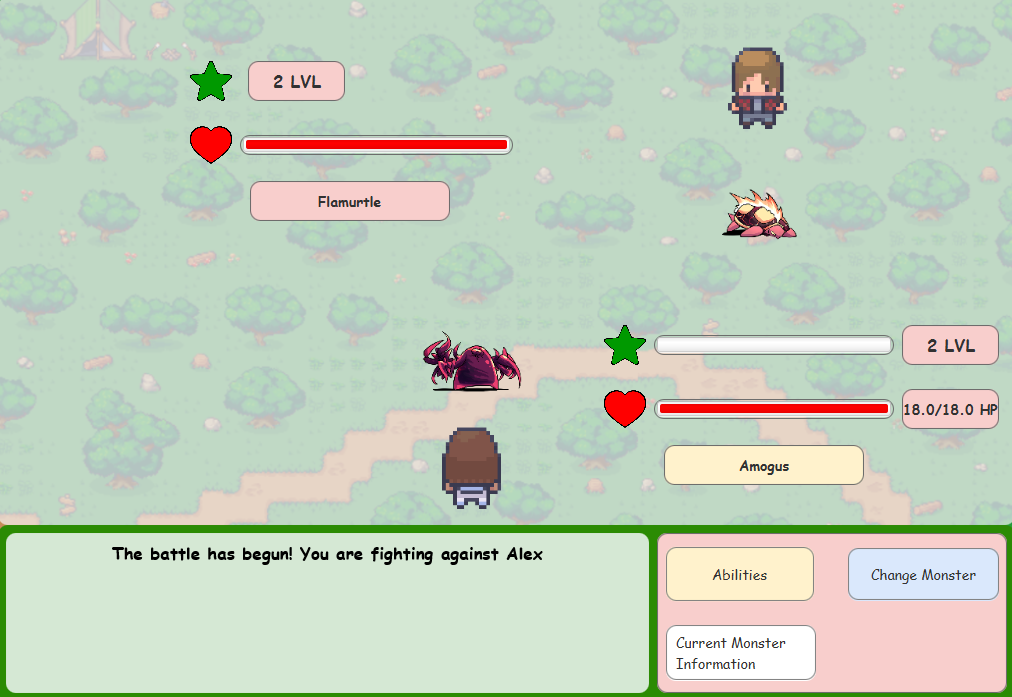
\includegraphics[width=\textwidth]{images/implementation/Encounter/1v1TrainervsTrainer.PNG}
        \caption{Implementierung: Eins-gegen-Eins Kampfsituation Trainer}
        \label{fig: Implementierung: Eins-gegen-Eins Kampfsituation Trainer}
    \end{subfigure}
    \caption{Vergleich: Eins-gegen-Eins Kampfsituation Trainer}
    \label{fig: Vergleich: Eins-gegen-Eins Kampfsituation Trainer}
\end{figure}
In der Abbildung~\ref{fig: Vergleich: Fähigkeiten des jetzigen Monsters} besteht ein Unterschied in der Darstellung der Fähigkeiten. Die Container der Fähigkeiten haben keine abgerundete Ecken. Der Unterschied dient nur der Ästhetik.

Beim Anwenden einer Fähigkeit wird das Ereignisprotokoll von dem Mockup verschieden dargestellt. Dabei wird der Text wie in der Abbildung~\ref{fig: Vergleich: Fähigkeit auf das gegnerische Monster angewandt} für die angewandte Fähigkeit des Gegners und des Trainers des Nutzers entsprechend aktualisiert. Das liegt daran, dass beide Parteien den Zug machen und somit das Ergebnis beider Fähigkeiten angezeigt werden muss. 
\begin{figure}[H]
    \centering
    \begin{subfigure}[b]{0.4\textwidth}
        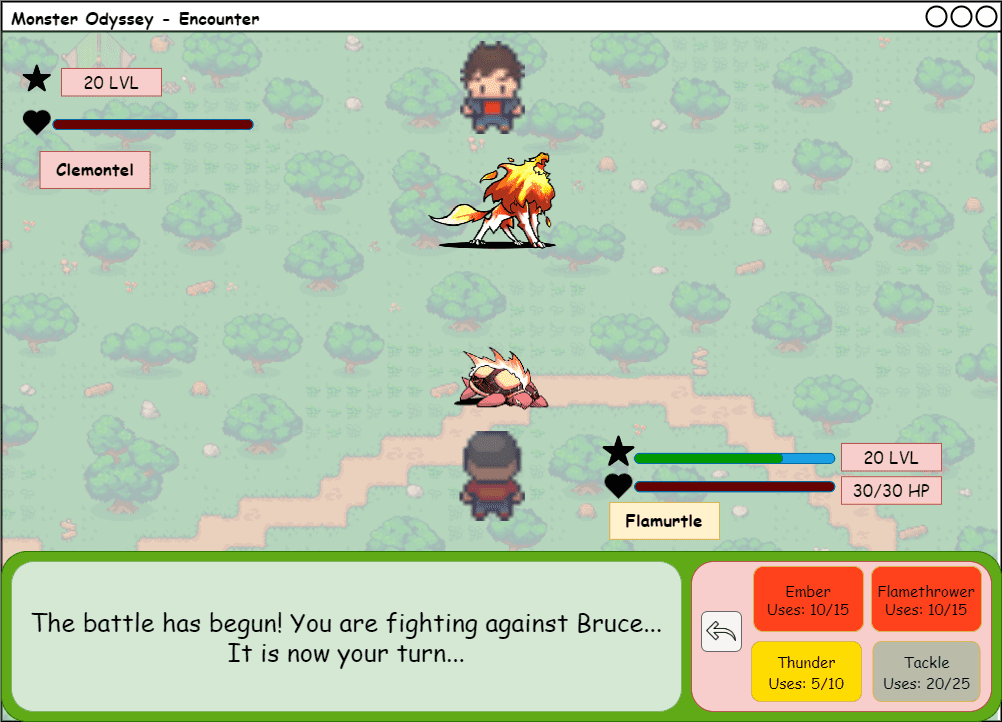
\includegraphics[width=\textwidth]{images/mockups/Encounter/Encounter1v1Abilities.png}
        \caption{Mockup: \phantom{desdes jetz}Fähigkeiten des jetzigen Monsters}
        \label{fig: Mockup: Fähigkeiten des jetzigen Monsters}
    \end{subfigure}
    \hfill
    \begin{subfigure}[b]{0.4\textwidth}
        \includegraphics[width=\textwidth]{images/implementation/Encounter/abilities.PNG}
        \caption{Implementierung: Fähigkeiten des jetzigen Monsters}
        \label{fig: Implementierung: Fähigkeiten des jetzigen Monsters}
    \end{subfigure}
    \caption{Vergleich: Fähigkeiten des jetzigen Monsters}
    \label{fig: Vergleich: Fähigkeiten des jetzigen Monsters}
\end{figure}
\begin{figure}[H]
    \centering
    \begin{subfigure}[b]{0.4\textwidth}
        \includegraphics[width=\textwidth]{images/mockups/Encounter/Encounter1v1AbilitiesUsed.png}
        \caption{Mockup: \phantom{gewandt} Fähigkeit angewandt}
        \label{fig: Mockup: Fähigkeit auf das gegnerische Monster angewandt}
    \end{subfigure}
    \hfill
    \begin{subfigure}[b]{0.4\textwidth}
        \includegraphics[width=\textwidth]{images/implementation/Encounter/abilitiesused.PNG}
        \caption{Implementierung: Fähigkeit angewandt}
        \label{fig: Implementierung: Fähigkeit auf das gegnerische Monster angewandt}
    \end{subfigure}
    \caption{Vergleich: Fähigkeit angewandt}
    \label{fig: Vergleich: Fähigkeit auf das gegnerische Monster angewandt}
\end{figure}
Zwischen den Mockups und der Implementierung beim Verlust oder Gewinn eines Kampfs bestehen zwei Unterschiede, die aufgrund von fehlender Qualitätssicherung wegen Zeitproblemen vor dem Releaseende enstanden sind. Zum einen wird das Fenster wie in der Abbildung~\ref{fig: Vergleich: Kampf verloren} größer als nötig dargestellt und zum anderen spiegelt sich der aktuelle Status des Kampfs nicht in dem Ereignisprotokoll wider.

In der Abbildung~\ref{fig: Vergleich: Levelup mit neuen Werten und neuer Fähigkeit} besteht bezüglich des Levelaufstiegs des eigenen Monsters ein Unterschied bei der Reihenfolge der geänderten Attribute. Die Reihenfolge ist dennoch für den Nutzer nicht ausschlaggebend und weist keine Funktionalitätsänderung auf. Darüber hinaus konnte die erworbene Fähigkeit nicht in dem designierten Bereich dargestellt werden, da es Zeitprobleme vor dem Releaseende beim Abschließen der entsprechenden User Story gegeben hat.
\begin{figure}[H]
    \centering
    \begin{subfigure}[b]{0.4\textwidth}
        \includegraphics[width=\textwidth]{images/mockups/Encounter/Encounter1v2OpponentAttackedAndLostPopup.png}
        \caption{Mockup: \phantom{Kampfve}Kampf verloren}
        \label{fig: Mockup: Kampf verloren}
    \end{subfigure}
    \hfill
    \begin{subfigure}[b]{0.4\textwidth}
        \includegraphics[width=\textwidth]{images/implementation/Encounter/encounterverloren.PNG}
        \caption{Implementierung: Kampf verloren}
        \label{fig: Implementierung: Kampf verloren}
    \end{subfigure}
    \caption{Vergleich: Kampf verloren}
    \label{fig: Vergleich: Kampf verloren}
\end{figure}
\begin{figure}[H]
    \centering
    \begin{subfigure}[b]{0.4\textwidth}
        \includegraphics[width=\textwidth]{images/mockups/Encounter/Encounter1v1AbilitiesUsedWonLevelUp.png}
        \caption{Mockup: Levelup}
        \label{fig: Mockup: Levelup mit neuen Werten und neuer Fähigkeit}
    \end{subfigure}
    \hfill
    \begin{subfigure}[b]{0.4\textwidth}
        \includegraphics[width=\textwidth]{images/implementation/Encounter/Levelupmitneuerability.PNG}
        \caption{Implementierung: Levelup}
        \label{fig: Implementierung: Levelup mit neuen Werten und neuer Fähigkeit}
    \end{subfigure}
    \caption{Vergleich: Levelup mit neuen Werten und neuer Fähigkeit}
    \label{fig: Vergleich: Levelup mit neuen Werten und neuer Fähigkeit}
\end{figure}
Bei dem Monsterwechsel-Fenster sind wie in der Abbildung~\ref{fig: Vergleich: Monster auswechseln Popup} zwei Unterschiede anzumerken. Hinter dem jeweiligen Monsterbild wird kein weißer Hintergrund dargestellt und die Bezeichnung für den Wechselknopf ist leicht unterschiedlich. Die Unterschiede dienen allerdings nur der Ästhetik und haben keinen Einfluss auf die Funktionalität.

In der Abbildung~\ref{fig: Vergleich: Popup beim Fliehen} ist das Popup für das Fliehen etwas größer als nötig gestaltet, wobei auch der Text für die Bestätigung anders als der Text im Mockup ist. Jedoch wird dabei die Semantik des Fliehens immer noch beibehalten. Die Änderungen betreffen die Funktionalität nicht.

Nach der Bestätigung des Fliehens wird der Text aus dem Ereignisprotokoll wie in der Abbildung~\ref{fig: Vergleich: Von wildem Monster geflohen} nicht identisch dargestellt. Das liegt daran, dass hierbei auch keine Qualitätssicherung aufgrund von fehlender Zeit vor dem Releaseende durchgeführt werden konnte. Darüber hinaus wird beim Fliehen eine flüssige Animation angezeigt, um das Fliehen zu visualisieren.
\begin{figure}[H]
    \centering
    \begin{subfigure}[b]{0.4\textwidth}
        \includegraphics[width=\textwidth]{images/mockups/Encounter/Encounter2v2ChangeMonsterPopup.png}
        \caption{Mockup: \phantom{wechseln}Monster auswechseln Popup}
        \label{fig: Mockup: Monster auswechseln Popup}
    \end{subfigure}
    \hfill
    \begin{subfigure}[b]{0.4\textwidth}
        \includegraphics[width=\textwidth]{images/implementation/Encounter/monsterwechseln.PNG}
        \caption{Implementierung: Monster auswechseln Popup}
        \label{fig: Implementierung: Monster auswechseln Popup}
    \end{subfigure}
    \caption{Vergleich: Monster auswechseln Popup}
    \label{fig: Vergleich: Monster auswechseln Popup}
\end{figure}
\begin{figure}[H]
    \centering
    \begin{subfigure}[b]{0.4\textwidth}
        \includegraphics[width=\textwidth]{images/mockups/Encounter/EncounterWildFleePopUp.png}
        \caption{Mockup: \phantom{beimFlie}Popup beim Fliehen}
        \label{fig: Mockup: Popup beim Fliehen}
    \end{subfigure}
    \hfill
    \begin{subfigure}[b]{0.4\textwidth}
        \includegraphics[width=\textwidth]{images/implementation/Encounter/fliehenpopup.PNG}
        \caption{Implementierung: Popup beim Fliehen}
        \label{fig: Implementierung: Popup beim Fliehen}
    \end{subfigure}
    \caption{Vergleich: Popup beim Fliehen}
    \label{fig: Vergleich: Popup beim Fliehen}
\end{figure}
\begin{figure}[H]
    \centering
    \begin{subfigure}[b]{0.4\textwidth}
        \includegraphics[width=\textwidth]{images/mockups/Encounter/EncounterWildFleed.png}
        \caption{Mockup: \phantom{desdes jetz}Von wildem Monster geflohen}
        \label{fig: Mockup: Von wildem Monster geflohen}
    \end{subfigure}
    \hfill
    \begin{subfigure}[b]{0.4\textwidth}
        \includegraphics[width=\textwidth]{images/implementation/Encounter/vomkampfgeflohen.PNG}
        \caption{Implementierung: Von wildem Monster geflohen}
        \label{fig: Implementierung: Von wildem Monster geflohen}
    \end{subfigure}
    \caption{Vergleich: Von wildem Monster geflohen}
    \label{fig: Vergleich: Von wildem Monster geflohen}
\end{figure}
\section{Monsterteam}\label{sec:monster-team}
Mit der Einführung der Funktion des Monsterteams ist die Verwaltung und die Übersicht der Monster leicht gemacht. 
Der Nutzer kann jederzeit seine Monster zum aktiven Team hinzufügen, entfernen und beliebig anordnen. 
Darüber hinaus kann der Nutzer die Monsterdetails des jeweiligen Monsters abrufen.
\subsection{Mockups}\label{subsec:mockups-monster-team}
Auf das Fenster des Monsterteams gelangt der Nutzer, wenn im Spielbildschirm der Knopf 'Monsters' gedrückt wird. 
Dabei erscheint zuerst der Inhalt der Registerkarte 'Active Team', in der das aktive Monsterteam wie in Abbildung~\ref{fig: Aktive Monster} dargestellt wird.
Alle Monster im aktiven Team haben den gleichen Aufbau: Das Monsterbild wird links angezeigt, dann folgen der Name, das Level und der Monster-Typ dieses Monsters.
Zudem gobt es vier Knöpfe wie in der Abbildung~\ref{fig: Aktive Monster} zu sehen ist: zwei Anordnungsknöpfe für die Reihenfolge der Monster, ein Knopf für das Entfernen aus dem aktiven Team und ein Knopf für das Anzeigen der Monsterdetails.
\begin{figure}[H]
    \center
    \includegraphics[scale=\scale]{images/mockups/Monster/IngameMonsterMonsterActiveWithoutFlamurtle.png}
    \caption{Mockup: Aktives Monsterteam}
    \label{fig: Aktive Monster}
\end{figure}
Zum Anzeigen der anderen Monster kann der Nutzer auf die Registerkarte 'Other' drücken. 
Dann wird der Inhalt des Fensters wie in Abbildung~\ref{fig: Andere Monster} aktualisiert, sodass die im aktiven Team nicht vorhandenen Monster angezeigt werden. 
Hier haben alle Monster den gleichen Aufbau wie im aktiven Team -- mit zwei klaren Unterschieden wie in den Abbildungen~\ref{fig: Aktive Monster} und~\ref{fig: Andere Monster}: Der 'Entfernen'-Knopf wird durch den 'Hinzufügen'-Knopf ersetzt und die Anordnungsknöpfe werden nicht angezeigt.
\begin{figure}[H]
    \center
    \includegraphics[scale=\scale]{images/mockups/Monster/IngameMonster.png}
    \caption{Mockup: Andere Monster}
    \label{fig: Andere Monster}
\end{figure}
Die Details von dem jeweiligen Monster können durch Drücken des Knopfs 'View Details' aufgerufen und angezeigt werden. Es erscheint das Fenster wie in der Abbildung~\ref{fig: Monsterdetails}. Der Aufbau der Monsterdetails folgt demselben Schema wie in der Abbildung~\ref{fig: Informationen über den jetzigen Monster}. In diesem Fall können für ein beliebiges Monster die Informationen abgerufen werden.
\begin{figure}[H]
    \center
    \includegraphics[scale=\scale]{images/mockups/Monster/IngameMonsterDetails.png}
    \caption{Mockup: Monsterdetails}
    \label{fig: Monsterdetails}
\end{figure}
Der Nutzer kann weiterhin ein beliebiges Monster zum aktiven Monsterteam beim Drücken des Knopfs 'Add to Active Team' hinzufügen. 
Es erscheint dabei ein Popup für die Bestätigung wie in Abbildung~\ref{fig: Monster zum aktiven Team hinzugefügt} und das gewählte Monster wird in die Registerkarte des aktiven Teams verschoben.
Jedoch besteht die Möglichkeit, dass das aktive Monsterteam bereits die maximale Anzahl von sechs Monstern besitzt. 
Dann erscheint wie in Abbildung~\ref{fig: Max. Limit Aktiven Teams} beim Drücken desselben Knopfs die Fehlermeldung, dass das gewählte Monster nicht zum aktiven Team hinzugefügt werden konnte.
\begin{figure}[H]
    \center
    \includegraphics[scale=\scale]{images/mockups/Monster/IngameMonsterMonsterAdded.png}
    \caption{Mockup: Monster zum aktiven Team hinzugefügt}
    \label{fig: Monster zum aktiven Team hinzugefügt}
\end{figure}
\begin{figure}[H]
    \center
    \includegraphics[scale=\scale]{images/mockups/Monster/IngameMonsterMonsterAddedMax.png}
    \caption{Mockup: Max. Limit Aktiven Teams}
    \label{fig: Max. Limit Aktiven Teams}
\end{figure}
Die Anordnung der Monster im aktiven Team besitzt eine relevante Rolle im Kampf. 
Das erste Monster in der Liste wird beim Kampfstart zum jetzigen Monster gesetzt. Hierdurch kann der Nutzer diese Eigenschaft mithilfe der Anordnung bevorzugt ausnutzen. 
Mit dem oberen Pfeilknopf kann das jeweilige Monster höher in der Liste gesetzt werden. Analog kann das jeweilige Monster mit dem unteren Pfeilknopf in der Liste weiter unten gesetzt werden. Die Abbildung~\ref{fig: Anordnung der Monster im aktiven Team} veranschaulicht, dass ein Monster aus der Abbildung~\ref{fig: Ursprüngliches aktives Team} eine Position nach unten gesetzt wird. Dadurch sieht das Ergebnis der Anordnung wie in Abbildung~\ref{fig: Anordnung geändert} aus.
\begin{figure}[H]
    \centering
    \begin{subfigure}[b]{0.4\textwidth}
        \includegraphics[width=\textwidth]{images/mockups/Monster/IngameMonsterMonster.png}
        \caption{Ursprüngliches aktives Team}
        \label{fig: Ursprüngliches aktives Team}
    \end{subfigure}
    \hfill
    \begin{subfigure}[b]{0.4\textwidth}
        \includegraphics[width=\textwidth]{images/mockups/Monster/IngameMonsterMoved.png}
        \caption{Anordnung geändert}
        \label{fig: Anordnung geändert}
    \end{subfigure}
    \caption{Mockup: Anordnung der Monster im aktiven Team}
    \label{fig: Anordnung der Monster im aktiven Team}
\end{figure}
Analog zum Hinzufügen von Monstern in das aktive Team kann der Nutzer beliebige Monster aus dem aktiven Team entfernen. 
Auf der Registerkarte 'Active Team' kann der Nutzer dies tun, indem er den Knopf 'Remove from Team' wie in Abbildung~\ref{fig: Ursprüngliches aktives Team} drückt. Infolgedessen erfolgt ein Popup wie in Abbildung~\ref{fig: Monster vom aktiven Team entfernt}, indem die Aktion bestätigt wird. 
\begin{figure}[H]
    \center
    \includegraphics[scale=\scale]{images/mockups/Monster/IngameMonsterMonsterActiveRemoved.png}
    \caption{Mockup: Monster vom aktiven Team entfernt}
    \label{fig: Monster vom aktiven Team entfernt}
\end{figure}
\subsection{Vergleich zwischen Mockups und Implementierung}\label{subsec:vergleich-zwischen-mockups-und-implementierung-monster-team}
In der Abbildung~\ref{fig: Vergleich: Monsterliste} bestehen grundsätzlich keine wesentlichen Unterschiede. Allerdings sind mehrere Elemente aus dem Mockup aus der Abbildung~\ref{fig: Mockup: Aktives Monsterteam} nicht vorhande. Demnach existieren beispielsweise die grüne Trennlinie unter den Registerkarten, die Umrandung um die Monsterliste und der weiße Hintergrund in der Implementierung aus der Abbildung~\ref{fig: Implementierung: Aktives Monsterteam} nicht. Diese Unterschiede dienen der Ästhetik und haben keine semantischen Konsequenzen auf das Spiel. Sie sind aufgrund von Zeitproblemen und niedriger Priorität nicht implementiert worden.
\begin{figure}[H]
    \centering
    \begin{subfigure}[b]{0.4\textwidth}
        \includegraphics[width=\textwidth]{images/mockups/Monster/IngameMonsterMonsterActiveWithoutFlamurtle.png}
        \caption{Mockup: Aktives Monsterteam \phantom{aaa}}
        \label{fig: Mockup: Aktives Monsterteam}
    \end{subfigure}
    \hfill
    \begin{subfigure}[b]{0.4\textwidth}
        \includegraphics[width=\textwidth]{images/implementation/Monster/Monsterteam Active.png}
        \caption{Implementierung: Aktives Monsterteam}
        \label{fig: Implementierung: Aktives Monsterteam}
    \end{subfigure}
    \caption{Vergleich: Monsterliste}
    \label{fig: Vergleich: Monsterliste}
\end{figure}
Ferner sind in der Abbildung~\ref{fig: Vergleich: Monsterdetails} einige weitere Unterschiede anzumerken. Neu hinzugekommen in der Implementierung in der Abbildung~\ref{fig: Implementierung: Monsterdetails} ist der Monstername unter dem Monsterbild, der für die Monsterdetails wichtig ist. Außerdem sind Trennlinien zwischen den Balken und den links- und rechtsliegenden Elementen hinzugefügt worden, um die Struktur des Fensters klar darzustellen. Die Balken aus dem Mockup in der Abbildung~\ref{fig: Mockup: Monsterdetails} sind schmal und mit blauem Hintergrund ausgestattet, wobei die Balken in der Implementierung etwas größer und mit weißem Hintergrund gestaltet sind. Zu den jeweiligen Balken sind die Attribute in der Implementierung als Wort ausgeschrieben, um das jeweilige Attribut in die entsprechende Sprache übersetzen zu können, sodass die angebotenen Sprachen immer noch unterstützt werden.
Des Weiteren ist der Monstertyp oben rechts wie in der Abbildung~\ref{fig: Implementierung: Monsterdetails} festgelegt, da die Übersetzungen in den angebotenen Sprachen Platz in Anspruch nehmen.
Zuletzt sind die Fähigkeiten des Monsters noch weiter voneinander getrennt, was dennoch keine Funktionalitätsänderung mit sich führt.
\begin{figure}[H]
    \centering
    \begin{subfigure}[b]{0.4\textwidth}
        \includegraphics[width=\textwidth]{images/mockups/Monster/IngameMonsterDetails.png}
        \caption{Mockup: \phantom{aaamonsterr} Monsterdetails}
        \label{fig: Mockup: Monsterdetails}
    \end{subfigure}
    \hfill
    \begin{subfigure}[b]{0.4\textwidth}
        \includegraphics[width=\textwidth]{images/implementation/Monster/Monsterdetails .png}
        \caption{Implementierung: Monsterdetails}
        \label{fig: Implementierung: Monsterdetails}
    \end{subfigure}
    \caption{Vergleich: Monsterdetails}
    \label{fig: Vergleich: Monsterdetails}
\end{figure}
\section{Erstes Bonusfeature: Audio-Ingame}\label{sec:audio-ingame}
Mit dem Kunden wurde als erstes Bonusfeature vereinbart, dass das Abspielen von Audio-Titeln in der Anwendung als Dauerschleife ermöglicht wird. 
Die Audio-Titel werden von dem Team 'Magical Studios' bereitgestellt, die zur jeweiligen Spielsituation und zum momentanen Bildschirm angepasst sind.
Dafür werden in den verschiedenen Bildschirmen verschiedene Audio-Titel abgespielt, die in der Tabelle~\ref{tab:audio} zu finden sind.
\subsection{Mockups}\label{subsec:mockups-audio-ingame}
Das Pausemenü wird in diesem Release mit dem 'Einstellungsmenü'-Knopf erweitert.
Das Fenster aus der Abbildung~\ref{fig: Pausemenü} erscheint, wenn der Nutzer auf den Knopf 'Pause' im Spielbildschirm drückt. 
Dabei ist wie in der Abbildung~\ref{fig: Pausemenü} der Knopf zum Fortsetzen des Spiels an erster Stelle, der Knopf zum Gelangen zum Einstellungsmenü an zweiter Stelle und der Knopf zum Verlassen des Spiels an letzter Stelle positioniert.
Beim Drücken des 'Einstellungsmenü'-Knopfs wird das Fenster aus der Abbildung~\ref{fig: Pausemenü} mit dem Fenster aus der Abbildung~\ref{fig: Einstellungsmenü} ersetzt. 
In diesem Fenster sind vier Knöpfe angezeigt: drei Knöpfe zum Öffnen der Ton-, Tastenkürzel- und Trainereinstellungen und ein Knopf zum Zurückkehren zum Pausemenü. Beim Drücken des 'Go Back'-Knopfs wird das Pausemenü erneut angezeigt.
Beim Öffnen der Toneinstellungen erscheint ein neues Fenster wie in Abbildung~\ref{fig: Audio-Einstellungen}, in dem eine Beschriftung für das Fenster, ein Schieberegler für die Verwaltung der Lautstärke und ein Knopf zum Schließen der Einstellungen beinhaltet sind. Beim Schließen der Einstellungen gelangt der Nutzer wieder zum Fenster aus Abbildung~\ref{fig: Einstellungsmenü}.
\begin{figure}[H]
    \center
    \includegraphics[scale=\scale]{images/mockups/Bonusfeatures/AudioIngame/IngameSettings.png}
    \caption{Mockup: Pausemenü}
    \label{fig: Pausemenü}
\end{figure}
\begin{figure}[H]
    \center
    \includegraphics[scale=\scale]{images/mockups/Bonusfeatures/AudioIngame/IngameSettingsMenu.png}
    \caption{Mockup: Einstellungsmenü}
    \label{fig: Einstellungsmenü}
\end{figure}
\begin{figure}[H]
    \center
    \includegraphics[scale=\scale]{images/mockups/Bonusfeatures/AudioIngame/AudioSettings.png}
    \caption{Mockup: Audio-Einstellungen}
    \label{fig: Audio-Einstellungen}
\end{figure}
Damit der Nutzer die Kontrolle über den Ton außerhalb des Spielbildschirms hat, sind zwei Knöpfe im Mainmenü- und Login-Bildschirm hinterlegt. Mithilfe dieser Knöpfe kann der Ton stummgeschaltet beziehungsweise die Stummschaltung aufgehoben werden. In der Abbildung~\ref{fig: Login-Bildschirm Audio-Knopf} wird der Knopf zum Stummschalten des Tons gedrückt. Hierdurch verwandelt wie in Abbildung~\ref{fig: Login-Bildschirm Audio-Knopf stumm} das Symbol, um mit dem aktuellen Status des Tons übereinzustimmen.
\begin{figure}[H]
    \centering
    \begin{subfigure}[b]{0.4\textwidth}
        \includegraphics[width=\textwidth]{images/mockups/Bonusfeatures/AudioIngame/Login.png}
        \caption{Login-Bildschirm Audio-Knopf}
        \label{fig: Login-Bildschirm Audio-Knopf}
    \end{subfigure}
    \hfill
    \begin{subfigure}[b]{0.4\textwidth}
        \includegraphics[width=\textwidth]{images/mockups/Bonusfeatures/AudioIngame/LoginMuted.png}
        \caption{Login-Bildschirm Audio-Knopf stumm}
        \label{fig: Login-Bildschirm Audio-Knopf stumm}
    \end{subfigure}
    \caption{Mockup: Login-Bildschirm}
    \label{fig: Login-Bildschirm}
\end{figure}
\subsection{Vergleich zwischen Mockups und Implementierung}\label{subsec:vergleich-zwischen-mockups-und-implementierung-audio-ingame}
Der einzig wesentliche Unterschied bei der Umsetzung dieser Anforderung ist, dass der Schieberegler für die Audio-Einstellungen in der Abbildung~\ref{fig: Implementierung: Audio-Einstellungen} etwas größer als in der Abbildung~\ref{fig: Mockup: Audio-Einstellungen} gestaltet ist. Dieser Unterschied ist  darauf zurückzuführen, dass sich das Konzipieren des Schiebereglers schwieriger als erwartet herausgestellt hat und aufgrund von Zeitprobleme weggelassen worden ist.
\begin{figure}[H]
    \centering
    \begin{subfigure}[b]{0.4\textwidth}
        \includegraphics[width=\textwidth]{images/mockups/Bonusfeatures/AudioIngame/AudioSettings.png}
        \caption{Mockup: \phantom{aaa} Audio-Einstellungen}
        \label{fig: Mockup: Audio-Einstellungen}
    \end{subfigure}
    \hfill
    \begin{subfigure}[b]{0.4\textwidth}
        \includegraphics[width=\textwidth]{images/implementation/Bonusfeatures/AudioIngame/audioingameimp.PNG}
        \caption{Implementierung: Audio-Einstellungen}
        \label{fig: Implementierung: Audio-Einstellungen}
    \end{subfigure}
    \caption{Vergleich: Bonusfeature Audio im Spiel}
    \label{fig: Vergleich: Bonusfeature Audio im Spiel}
\end{figure}
Des Weiteren ist in den Abbildungen~\ref{fig: Vergleich: Pausemenü} und~\ref{fig: Vergleich: Einstellungsmenü} anzumerken, dass die Implementierungen mit den Mockups für das Pause-/Einstellungsmenü identisch sind. 
\begin{figure}[H]
    \centering
    \begin{subfigure}[b]{0.4\textwidth}
        \includegraphics[width=\textwidth]{images/mockups/Bonusfeatures/AudioIngame/IngameSettings.png}
        \caption{Mockup: Pausemenü}
        \label{fig: Mockup: Pausemenü}
    \end{subfigure}
    \hfill
    \begin{subfigure}[b]{0.4\textwidth}
        \includegraphics[width=\textwidth]{images/implementation/Bonusfeatures/AudioIngame/Pausemenu imp.png}
        \caption{Implementierung: Pausemenü}
        \label{fig: Implementierung: Pausemenü}
    \end{subfigure}
    \caption{Vergleich: Pausemenü}
    \label{fig: Vergleich: Pausemenü}
\end{figure}
\begin{figure}[H]
    \centering
    \begin{subfigure}[b]{0.4\textwidth}
        \includegraphics[width=\textwidth]{images/mockups/Bonusfeatures/AudioIngame/IngameSettingsMenu.png}
        \caption{Mockup: ~\phantom{aaaaaa} Einstellungsmenü}
        \label{fig: Mockup: Einstellungsmenü}
    \end{subfigure}
    \hfill
    \begin{subfigure}[b]{0.4\textwidth}
        \includegraphics[width=\textwidth]{images/implementation/Bonusfeatures/AudioIngame/Settingsmenu imp.png}
        \caption{Implementierung: Einstellungsmenü}
        \label{fig: Implementierung: Einstellungsmenü}
    \end{subfigure}
    \caption{Vergleich: Einstellungsmenü}
    \label{fig: Vergleich: Einstellungsmenü}
\end{figure}
\section{Zweites Bonusfeature: Hilfestellung zur aktuellen Spielsituation}\label{sec:handy-help}
Das Spiel \textit{ Monster Odyssey} wird mit diesem Bonusfeature einsteigerfreundlicher, da der Nutzer beim ersten Einstieg in das Spiel eine kurze Einführung über das Spiel und die Tastenkombinationen mittels eines modernen, futuristischen Handys erhält. Darüber hinaus erhält der Nutzer Unterstützung in bestimmten Situationen. Beispielsweise erscheinen einige Benachrichtigungen beziehunsgweise Hilfestellungen, nachdem der Nutzer das Starter-Monster erhalten oder der Nutzer einen Kampf verloren hat und seine Monster keine Lebenspunkte mehr haben.
\subsection{Mockups}\label{subsec:mockups-handy-help}
Wenn der Nutzer zum ersten Mal in das Spiel einsteigt, erscheint eine Glocke oben rechts, wie in Abbildung~\ref{fig: Benachrichtigung beim Erhalt einer Nachricht} neben dem futuristischen Handy zu sehen ist.
Die Glocke bedeutet, dass es mindestens eine ungelesene Nachricht von dem Alien Meruem gibt.
Der Nutzer kann diese Nachrichten lesen, indem er in der oberen rechten Ecke auf das Handy, wie in der Abbildung~\ref{fig: Benachrichtigung beim Erhalt einer Nachricht} drückt. 
Meruem hat bereits bei der Willkommensszene dem Nutzer geholfen und somit ist er auch im Spiel der Begleiter des Nutzers.
Zuerst begrüßt Meruem den Nutzer und heißt ihn in das Spiel willkommen.
Danach hinterlässt Meruem als Hilfestellung Nachrichten bei dem Nutzer. Meruem teilt dem Nutzer zum Beispiel mit, dass er seinen Trainer bewegen kann und welche Interaktionstaste gewählt ist. 
Darüber hinaus verweist er den Nutzer auf den NPC-Trainer Prof. Albert, bei dem Starter-Monster erworben werden können. Eine Beispieldarstellung dieser Nachrichten ist in der Abbildung~\ref{fig: Vierte Nachricht} zu finden.
\begin{figure}[H]
    \center
    \includegraphics[scale=\scale]{images/mockups/Bonusfeatures/Helpsituation/PlayerAndPlayerIngame.png}
    \caption{Mockup: Benachrichtigungssymbol beim Erhalt einer Nachricht}
    \label{fig: Benachrichtigung beim Erhalt einer Nachricht}
\end{figure}
\begin{figure}[H]
        \center
        \includegraphics[scale=\scale]{images/mockups/Bonusfeatures/Helpsituation/PlayerAndPlayerIngameFourthNotification.png}
        \caption{Hilfestellung beim Einstieg}
        \label{fig: Vierte Nachricht}
\end{figure}
Der Nutzer erhält von Meruem Nachrichten nach bestimmten Ereignissen.
Beispielsweise bekommt der Nutzer nach dem Erhalt von dem Starter-Monster zwei Nachrichten von Meruem wie in der Abbildung~\ref{fig: Sechste Nachricht}, in denen der Nutzer aufgerufen wird, seine Fähigkeiten unter Beweis zu stellen, mit anderen Trainern zu interagieren und gegen diese zu kämpfen.
Weiterhin erhält der Nutzer Hilfestellung von Meruem nach dem Verlust eines Kampfs oder bei niedrigen Lebenspunkten der eigenen Monster wie in der Abbildung~\ref{fig: Achte Nachricht}, indem Meruem den Nutzer auf die Krankenschwester im 'Moncenter' verweist, um die Monster zu heilen.
\begin{figure}[H]
        \center
        \includegraphics[scale=\scale]{images/mockups/Bonusfeatures/Helpsituation/PlayerAndPlayerIngameSixthNotification.png}
        \caption{Hilfestellung beim Erhalt eines Starter-Monsters}
        \label{fig: Sechste Nachricht}
\end{figure}
\begin{figure}[H]
        \center
        \includegraphics[scale=\scale]{images/mockups/Bonusfeatures/Helpsituation/PlayerAndPlayerIngameEigthNotification.png}
        \caption{Hilfestellung bei niedrigen Lebenspunkten der Monster}
        \label{fig: Achte Nachricht}
\end{figure}
\subsection{Vergleich zwischen Mockups und Implementierung}\label{subsec:vergleich-zwischen-mockups-und-implementierung-handy-help}
In der Abbildung~\ref{fig: Vergleich: Einstiegshilfe} bestehen zwischen dem Mockup und der Implementierung zwei Unterschiede. Zunächst enthält der Knopf für das Schließen in der Abbildung~\ref{fig: Implementierung: Einstiegshilfe} nur den Text 'Close', da bei der Übersetzung in die angebotenen Sprachen der Text viel Platz in Anspruch genommen hätte. Außerdem hat das Bild für Meruem keinen Behälter, was allerdings keinen Einfluss auf die Mechanik oder das Spielerlebnis hat. Dieser wurde wegen zunehmender Komplexität des Handys und der Nachrichten weggelassen.
\begin{figure}[H]
    \centering
    \begin{subfigure}[b]{0.4\textwidth}
        \includegraphics[width=\textwidth]{images/mockups/Bonusfeatures/Helpsituation/PlayerAndPlayerIngameFourthNotification.png}
        \caption{Mockup: Einstiegshilfe}
        \label{fig: Mockup: Einstiegshilfe}
    \end{subfigure}
    \hfill
    \begin{subfigure}[b]{0.4\textwidth}
        \includegraphics[width=\textwidth]{images/implementation/Bonusfeatures/Helpsituation/FirstMessagesImp.png}
        \caption{Implementierung: Einstiegshilfe}
        \label{fig: Implementierung: Einstiegshilfe}
    \end{subfigure}
    \caption{Vergleich: Einstiegshilfe}
    \label{fig: Vergleich: Einstiegshilfe}
\end{figure}
Überdies besteht noch ein wesentlicher Unterschied beim Vergleich in der Abbildung~\ref{fig: Vergleich: Nach Erhalt des Starter-Monsters} bezüglich der Hilfestellung nach Auftreten eines Ereignisses. Hierfür wurden die vorherigen Nachrichten in der Implementierung entfernt, um das Handy nicht dauherhaft zu überladen. Das erleichtert das Lesen der Nachrichten auf dem Handy.
\begin{figure}[H]
    \centering
    \begin{subfigure}[b]{0.4\textwidth}
        \includegraphics[width=\textwidth]{images/mockups/Bonusfeatures/Helpsituation/PlayerAndPlayerIngameSixthNotification.png}
        \caption{Mockup: Nach Erhalt des Starter-Monsters}
        \label{fig: Mockup: Nach Erhalt des Starter-Monsters}
    \end{subfigure}
    \hfill
    \begin{subfigure}[b]{0.4\textwidth}
        \includegraphics[width=\textwidth]{images/implementation/Bonusfeatures/Helpsituation/StarterMonsterMessagesImp.png}
        \caption{Implementierung: Nach Erhalt des Starter-Monsters}
        \label{fig: Implementierung: Nach Erhalt des Starter-Monsters}
    \end{subfigure}
    \caption{Vergleich: Nach Erhalt des Starter-Monsters}
    \label{fig: Vergleich: Nach Erhalt des Starter-Monsters}
\end{figure}
\section{Drittes Bonusfeature: Einstellungen der Tastenkürzel}\label{sec:keybindings-settings}
Die Tastenkürzel selbst festzulegen ist Bestandteil von vielen Spielen, daher wurde mit dem Kunden vereinbart, Einstellungen für die Tastenkürzel als drittes Bonusfeature zu entwickeln. Der Nutzer kann somit gewünschte Tasten für die Bewegung, Interaktion und das Öffnen des Pausemenüs festlegen. 
\subsection{Mockups}\label{subsec:mockups-keybindings-settings}
Das Einstellungsfenster für die Tastenkombinationen aus der Abbildung~\ref{fig: Einstellungen der Tastenkürzel} kann der Nutzer öffnen, indem er auf den Knopf 'Keybindings' in dem Einstellungsmenü aus der Abbildung~\ref{fig: Einstellungsmenü} drückt.
In der Abbildung~\ref{fig: Einstellungen der Tastenkürzel} sieht der Nutzer verschiedene Knöpfe, die einen Inhaltstext von der jetzig festgelegten Taste besitzen: vier Knöpfe für die Navigation, einen Knopf für die Interaktion und einen Knopf für das Öffnen des Pausemenüs. Darüber hinaus sind noch drei andere Knöpfe vorhanden, um jeweils zum Einstellungsmenü zurückzukehren, alle Tasten auf die voreingestellten Tastenkombinationen zurückzusetzen oder die Änderungen der Tastenkombinationen zu bestätigen.
\begin{figure}[H]
    \center
    \includegraphics[scale=\scale]{images/mockups/Bonusfeatures/Keybindings/KeybindingsSettings.png}
    \caption{Mockup: Einstellungen der Tastenkürzel}
    \label{fig: Einstellungen der Tastenkürzel}
\end{figure}
\begin{figure}[H]
    \center
    \includegraphics[scale=\scale]{images/mockups/Bonusfeatures/Keybindings/KeybindingsSettingsDefault.png}
    \caption{Mockup: Tastenkürzel zurückgesetzt}
    \label{fig: Tastenkürzel zurückgesetzt}
\end{figure}
Sobald der Nutzer beispielsweise einen Knopf der Navigationstasten drückt, wird der Inhaltstext dieser Taste mit „...“ wie in der Abbildung~\ref{fig: Knopf gedrückt} ersetzt und wird auf eine Eingabe vom Nutzer gewartet. Dabei wird der Nutzer zusätzlich in einem Text wie in Abbildung~\ref{fig: Knopf gedrückt} darauf hingewiesen, dass auf eine Eingabe gewartet wird. Der Inhaltstext wird mit der entsprechenden Taste, wie in Abbildung~\ref{fig: Tastenkürzel geändert} ersetzt, und ein Text für die Bestätigung angezeigt, wenn die Eingabe vom Nutzer erfolgt ist. Anschließend kann der Nutzer auf dem blauen Knopf aus der Abbildung~\ref{fig: Tastenkürzel geändert} drücken, um die Änderungen abzuschließen und zu speichern.
Möchte der Nutzer zu einem späteren Zeitpunkt mit den voreingestellten Tastenkombinationen weiterspielen, so kann er dies mit dem mittleren Knopf aus der Abbildung~\ref{fig: Einstellungen der Tastenkürzel} tuen. Es wird dabei die Aktion mit einem Text in demselben Fenster wie in der Abbildung~\ref{fig: Tastenkürzel zurückgesetzt} bestätigt.
\begin{figure}[H]
    \centering
    \begin{subfigure}[b]{0.4\textwidth}
        \includegraphics[width=\textwidth]{images/mockups/Bonusfeatures/Keybindings/KeybindingsSettingsWaitingForInput.png}
        \caption{Mockup: Knopf gedrückt}
        \label{fig: Knopf gedrückt}
    \end{subfigure}
    \hfill
    \begin{subfigure}[b]{0.4\textwidth}
        \includegraphics[width=\textwidth]{images/mockups/Bonusfeatures/Keybindings/KeybindingsSettingsChanged.png}
        \caption{Mockup: Tastenkürzel geändert}
        \label{fig: Tastenkürzel geändert}
    \end{subfigure}
    \caption{Mockup: Ändern eines Tastenkürzels}
    \label{fig: Ändern eines Tastenkürzels}
\end{figure}
\subsection{Vergleich zwischen Mockups und Implementierung}\label{subsec:vergleich-zwischen-mockups-und-implementierung-keybindings-settings}
In der Abbildung~\ref{fig: Vergleich: Einstellungen der Tastenkürzel} sind zwei Unterschiede zwischen dem Mockup und der Implementierung anzudeuten: Der Hinweis für das Ändern der Tastenkürzel wird in der Implementierung wie in der Abbildung~\ref{fig: Implementierung: Einstellungen der Tastenkürzel} nicht kursiv geschrieben, was dennoch keinen Einfluss auf die Logik der Einstellungen hat. Zudem ändert sich nach Rücksprache mit dem Kunden der Standardknopf für das Pausieren des Spiels auf die Taste „ESC“.
\begin{figure}[H]
    \centering
    \begin{subfigure}[b]{0.4\textwidth}
        \includegraphics[width=\textwidth]{images/mockups/Bonusfeatures/Keybindings/KeybindingsSettings.png}
        \caption{Mockup: Einstellungen der Tastenkürzel}
        \label{fig: Mockup: Einstellungen der Tastenkürzel}
    \end{subfigure}
    \hfill
    \begin{subfigure}[b]{0.4\textwidth}
        \includegraphics[width=\textwidth]{images/implementation/Bonusfeatures/Keybindings/SettingsKeyImp.png}
        \caption{Implementierung: Einstellungen der Tastenkürzel}
        \label{fig: Implementierung: Einstellungen der Tastenkürzel}
    \end{subfigure}
    \caption{Vergleich: Einstellungen der Tastenkürzel}
    \label{fig: Vergleich: Einstellungen der Tastenkürzel}
\end{figure}
Des Weiteren besteht in der Abbildung~\ref{fig: Vergleich: Warten auf Eingabe} ein wesentlicher Unterschied zwischen dem Mockup und der Implementierung. Beim Drücken einer Taste werden die anderen Tasten in der Implementierung wie in der Abbildung~\ref{fig: Implementierung: Warten auf Eingabe} kurzzeitig deaktiviert, damit der Nutzer keine andere Taste gleichzeitig ändern kann. Außerdem wird der Hinweistext im Fenster nicht zentriert, was dennoch keine Funktionalitätsänderung mit sich führt.
\begin{figure}[H]
    \centering
    \begin{subfigure}[b]{0.4\textwidth}
        \includegraphics[width=\textwidth]{images/mockups/Bonusfeatures/Keybindings/KeybindingsSettingsWaitingForInput.png}
        \caption{Mockup: \phantom{aaaaaaa} Warten auf Eingabe}
        \label{fig: Mockup: Warten auf Eingabe}
    \end{subfigure}
    \hfill
    \begin{subfigure}[b]{0.4\textwidth}
        \includegraphics[width=\textwidth]{images/implementation/Bonusfeatures/Keybindings/WaitForInput.png}
        \caption{Implementierung: Warten auf Eingabe}
        \label{fig: Implementierung: Warten auf Eingabe}
    \end{subfigure}
    \caption{Vergleich: Warten auf Eingabe}
    \label{fig: Vergleich: Warten auf Eingabe}
\end{figure}
Zuletzt ist in der Abbildung~\ref{fig: Vergleich: Eingabe erfolgt} ein weiterer wichtiger Unterschied zu sehen: Die Tastenänderung erfolgt vom Nutzer in der Implementierung wie in der Abbildung~\ref{fig: Implementierung: Eingabe erfolgt} nur dann, wenn der Nutzer den Bestätigungsknopf gedrückt hat. Somit kann der Nutzer selbst entscheiden, ob er seine Änderungen rückgängig machen möchte, die er getätigt hatte.
\begin{figure}[H]
    \centering
    \begin{subfigure}[b]{0.4\textwidth}
        \includegraphics[width=\textwidth]{images/mockups/Bonusfeatures/Keybindings/KeybindingsSettingsChanged.png}
        \caption{Mockup: \phantom{aaaaaaa} Eingabe erfolgt}
        \label{fig: Mockup: Eingabe erfolgt}
    \end{subfigure}
    \hfill
    \begin{subfigure}[b]{0.4\textwidth}
        \includegraphics[width=\textwidth]{images/implementation/Bonusfeatures/Keybindings/InputErfolgt.png}
        \caption{Implementierung: Eingabe erfolgt}
        \label{fig: Implementierung: Eingabe erfolgt}
    \end{subfigure}
    \caption{Vergleich: Eingabe erfolgt}
    \label{fig: Vergleich: Eingabe erfolgt}
\end{figure}

\section{Erweiterung: Trainereinstellungen}\label{sec:trainer-settings}
Zuletzt ist mit dem Kunden vereinbart worden, die Anforderung 'Trainererstellung' aus dem zweiten Release zu erweitern, sodass der Nutzer seinen Trainer jederzeit bearbeiten kann. Der Nutzer kann somit nicht nur den Trainer löschen, sondern nun auch den Namen oder den Charakter des Trainers bearbeiten.
\subsection{Mockups}\label{subsec:mockups-trainer-settings}
Die Trainereinstellungen kann der Nutzer navigieren, indem der Knopf 'Trainer Settings' aus Abbildung~\ref{fig: Einstellungsmenü} gedrückt wird. Dabei erscheint das Fenster aus der Abbildung~\ref{fig: Trainereinstellungen}. In dem Fenster ist ein Textfeld für die Bearbeitung des Trainernamen zu sehen. Anschließend folgt ein Bild des jetzigen Trainer-Charakters. Die anderen Charaktere kann der Nutzer sehen, sobald er auf den rechten beziehungsweise den linken Pfeilknopf drückt. Darüber hinaus existieren zwei Knöpfe auf der unteren Seite des Fensters: ein Knopf für das Aktualisieren mit den von dem Nutzer geänderten Eingaben und ein Knopf für das Löschen des Trainers.
Falls der Nutzer Änderungen an seinem Trainer vorgenommen hat und auf den Knopf 'Update Trainer' aus der Abbildung~\ref{fig: Trainereinstellungen} drückt, dann erscheint ein Popup wie in Abbildung~\ref{fig: Trainer aktualisiert}. In diesem Popup bekommt der Nutzer die Bestätigung, dass die Änderungen erfolgreich gespeichert sind und das Spiel beim Drücken des Knopfs 'OK' neu gestartet wird.
Möchte der Nutzer seinen Trainer endgültig löschen, dann kann er beim Drücken des Knopfs 'Delete Trainer' aus der Abbildung~\ref{fig: Trainereinstellungen} die gewünschte Aktion erzielen. Dabei erscheint ein Popup wie in Abbildung~\ref{fig: Popup beim Löschen des Trainers} für die Bestätigung der Aktion, das eine Eingabe von dem Nutzer erwartet. Beim Drücken des Knopfs 'Cancel' aus der Abbildung~\ref{fig: Popup beim Löschen des Trainers} wird die Aktion für nichtig erklärt. Beim Drücken des Knopfs 'OK' wird der Trainer von dem Server gelöscht und es wird auf den Mainmenü-Bildschirm wie in Abbildung~\ref{fig: Trainer erfolgreich gelöscht} gewechselt. Außerdem ist ein Bestätigungstext für die Aktion in dem Mainmenü-Bildschirm wie in der Abbildung~\ref{fig: Trainer erfolgreich gelöscht} angezeigt.
\begin{figure}[H]
    \centering
    \begin{subfigure}[b]{0.4\textwidth}
        \includegraphics[width=\textwidth]{images/mockups/Bonusfeatures/TrainerSettings/TrainerSetting.png}
        \caption{Trainereinstellungen}
        \label{fig: Trainereinstellungen}
    \end{subfigure}
    \hfill
    \begin{subfigure}[b]{0.4\textwidth}
        \includegraphics[width=\textwidth]{images/mockups/Bonusfeatures/TrainerSettings/TrainerSettingChanged.png}
        \caption{Trainer aktualisiert}
        \label{fig: Trainer aktualisiert}
    \end{subfigure}
    \caption{Mockup: Aktualisieren des Trainers}
    \label{fig: Aktualisieren des Trainers}
\end{figure}
\begin{figure}[H]
    \centering
    \begin{subfigure}[b]{0.4\textwidth}
        \includegraphics[width=\textwidth]{images/mockups/Bonusfeatures/TrainerSettings/IngameDeleteTrainerPopup.png}
        \caption{Popup für Löschen des Trainers}
        \label{fig: Popup beim Löschen des Trainers}
    \end{subfigure}
    \hfill
    \begin{subfigure}[b]{0.4\textwidth}
        \includegraphics[width=\textwidth]{images/mockups/Bonusfeatures/TrainerSettings/TrainerAccountDeleted.png}
        \caption{Trainer erfolgreich gelöscht}
        \label{fig: Trainer erfolgreich gelöscht}
    \end{subfigure}
    \caption{Mockup: Löschen des Trainers}
    \label{fig: Löschen des Trainers}
\end{figure}
\subsection{Vergleich zwischen Mockups und Implementierung}\label{subsec:vergleich-zwischen-mockups-und-implementierung-trainer-settings}
Die Mockups sind mit der Implementierung übereinstimmend, bis auf das Mockup in der Abbildung~\ref{fig: Trainer erfolgreich gelöscht}. Dafür ist in der Abbildung~\ref{fig: Mockup: Trainer erfolgreich gelöscht} der Audio-Button in der Abbildung~\ref{fig: Implementierung: Trainer erfolgreich gelöscht} fehlend und der Bestätigungstext für das Löschen des Trainers befindet sich über dem Startknopf des Spiels. Der Bestätigungstext in der Abbildung~\ref{fig: Implementierung: Trainer erfolgreich gelöscht} unterscheidet sich ebenso. Dennoch besitzt der Unterschied keine semantischen Folgen. Somit hat der Text dieselbe Semantik wie in der Abbildung~\ref{fig: Mockup: Trainer erfolgreich gelöscht}. 
\begin{figure}[H]
    \centering
    \begin{subfigure}[b]{0.4\textwidth}
        \includegraphics[width=\textwidth]{images/mockups/Bonusfeatures/TrainerSettings/TrainerAccountDeleted.png}
        \caption{Mockup: Trainer erfolgreich gelöscht}
        \label{fig: Mockup: Trainer erfolgreich gelöscht}
    \end{subfigure}
    \hfill
    \begin{subfigure}[b]{0.4\textwidth}
        \includegraphics[width=\textwidth]{images/implementation/Bonusfeatures/TrainerSettings/Trainerdeleted.PNG}
        \caption{Implementierung: Trainer erfolgreich gelöscht}
        \label{fig: Implementierung: Trainer erfolgreich gelöscht}
    \end{subfigure}
    \caption{Vergleich: Erweiterung Trainereinstellungen}
    \label{fig: Vergleich: Erweiterung Trainereinstellungen}
\end{figure}
In den Abbildungen~\ref{fig: Vergleich: Trainereinstellungen},~\ref{fig: Vergleich: Trainer aktualisiert} und~\ref{fig: Vergleich: Popup für Löschen des Trainers} ist zu sehen, dass es keine bis geringfügige Unterschiede zwischen den Mockups und der Implementierung gibt, wobei die kleinen Unterscheide keinen Einfluss auf die Funktionalität haben.
\begin{figure}[H]
    \centering
    \begin{subfigure}[b]{0.4\textwidth}
        \includegraphics[width=\textwidth]{images/mockups/Bonusfeatures/TrainerSettings/TrainerSetting.png}
        \caption{Mockup: \phantom{Trainer} Trainereinstellungen}
        \label{fig: Mockup: Trainereinstellungen}
    \end{subfigure}
    \hfill
    \begin{subfigure}[b]{0.4\textwidth}
        \includegraphics[width=\textwidth]{images/implementation/Bonusfeatures/TrainerSettings/TrainerSettings.png}
        \caption{Implementierung: Trainereinstellungen}
        \label{fig: Implementierung: Trainereinstellungen}
    \end{subfigure}
    \caption{Vergleich: Trainereinstellungen}
    \label{fig: Vergleich: Trainereinstellungen}
\end{figure}
\begin{figure}[H]
    \centering
    \begin{subfigure}[b]{0.4\textwidth}
        \includegraphics[width=\textwidth]{images/mockups/Bonusfeatures/TrainerSettings/TrainerSettingChanged.png}
        \caption{Mockup: \phantom{Trainer} Trainer aktualisiert}
        \label{fig: Mockup: Trainer aktualisiert}
    \end{subfigure}
    \hfill
    \begin{subfigure}[b]{0.4\textwidth}
        \includegraphics[width=\textwidth]{images/implementation/Bonusfeatures/TrainerSettings/UpdateTrainer.png}
        \caption{Implementierung: Trainer aktualisiert}
        \label{fig: Implementierung: Trainer aktualisiert}
    \end{subfigure}
    \caption{Vergleich: Trainer aktualisiert}
    \label{fig: Vergleich: Trainer aktualisiert}
\end{figure}
\begin{figure}[H]
    \centering
    \begin{subfigure}[b]{0.4\textwidth}
        \includegraphics[width=\textwidth]{images/mockups/Bonusfeatures/TrainerSettings/IngameDeleteTrainerPopup.png}
        \caption{Mockup: Popup für Löschen des Trainers}
        \label{fig: Mockup: Popup beim Löschen des Trainers}
    \end{subfigure}
    \hfill
    \begin{subfigure}[b]{0.4\textwidth}
        \includegraphics[width=\textwidth]{images/implementation/Bonusfeatures/TrainerSettings/DeleteTrainer.png}
        \caption{Implementierung: Popup für Löschen des Trainers}
        \label{fig: Implementierung: Popup für Löschen des Trainers}
    \end{subfigure}
    \caption{Vergleich: Popup für Löschen des Trainers}
    \label{fig: Vergleich: Popup für Löschen des Trainers}
\end{figure}